\documentclass[12pt]{report}
\usepackage{graphicx}     %standard package. Note graphics<graphicx<epsfig
\usepackage{color}     %standard package
\usepackage{hyperref} %standard package written by Sebastian Rahtz
%\usepackage{subeqn}    %allows equations 1a, 1b
%\usepackage{subfig}    %allows figures 1a, 1b
\usepackage{amsmath}
\usepackage{amssymb}
\usepackage{url} 
\usepackage{bbm}%for indicator function

\usepackage[nottoc]{tocbibind}

\usepackage[color,matrix,frame,arrow]{xy}
\usepackage[table,xcdraw]{xcolor}
\usepackage[shortlabels]{enumitem}
\usepackage{array}
\usepackage{pdflscape}


\paperheight=11in
\topmargin=0in
\headheight=0in
\headsep=0in
\topskip=0in
\textheight=8.5in
\footskip=.5in

\paperwidth=8.5in
\oddsidemargin=0in
\evensidemargin=0in
\textwidth=7.0in
\parindent=.5in

\newtheorem{claim}{Claim}
\newcommand{\proof}[0]{{\bf proof:} }
\newcommand{\qed}[0]{\newline\noindent{\bf QED }}


\newcommand{\bra}[1]{\langle#1|}
\newcommand{\ket}[1]{|#1\rangle}
\newcommand{\av}[1]{\langle#1\rangle}
\newcommand{\pder}[2]{\frac{\partial#1}{\partial#2}}
\newcommand{\tr}[0]{{\rm tr }}
\newcommand{\beq}{\begin{equation}}
\newcommand{\eeq}{\end{equation}}
\newcommand{\bsub}{\begin{subequations}}
	\newcommand{\esub}{\end{subequations}}
\newcommand{\beqa}{\begin{eqnarray}}
\newcommand{\eeqa}{\end{eqnarray}}
\newcommand{\rarrow}[0]{\rightarrow}
\newcommand{\larrow}[0]{\leftarrow}
\newcommand{\Rarrow}[0]{\Rightarrow}
\newcommand{\nRarrow}[0]{\nRightarrow}
\newcommand{\Larrow}[0]{\Leftarrow}
\newcommand{\nLarrow}[0]{\nLeftarrow}
\newcommand{\ul}[1]{\underline{#1}}
\newcommand{\ol}[1]{\overline{#1}}
\newcommand{\ZZ}[0]{ {\mathbb{Z}}}
\newcommand{\RR}[0]{{ \mathbb{R}} }
\newcommand{\CC}[0]{{ \mathbb{C}} }
\newcommand{\ground}{{}_{\stackrel{\stackrel{\displaystyle{\bot}}{-}}{.}}}


\newcommand{\rva}[0]{{\ul{a}}}
\newcommand{\rvb}[0]{{\ul{b}}}
\newcommand{\rvc}[0]{{\ul{c}}}
\newcommand{\rvd}[0]{{\ul{d}}}
\newcommand{\rve}[0]{{\ul{e}}}
\newcommand{\rvf}[0]{{\ul{f}}}
\newcommand{\rvg}[0]{{\ul{g}}}
\newcommand{\rvh}[0]{{\ul{h}}}
\newcommand{\rvi}[0]{{\ul{i}}}
\newcommand{\rvj}[0]{{\ul{j}}}
\newcommand{\rvk}[0]{{\ul{k}}}
\newcommand{\rvl}[0]{{\ul{l}}}
\newcommand{\rvm}[0]{{\ul{m}}}
\newcommand{\rvn}[0]{{\ul{n}}}
\newcommand{\rvo}[0]{{\ul{o}}}
\newcommand{\rvp}[0]{{\ul{p}}}
\newcommand{\rvq}[0]{{\ul{q}}}
\newcommand{\rvr}[0]{{\ul{r}}}
\newcommand{\rvs}[0]{{\ul{s}}}
\newcommand{\rvt}[0]{{\ul{t}}}
\newcommand{\rvu}[0]{{\ul{u}}}
\newcommand{\rvv}[0]{{\ul{v}}}
\newcommand{\rvw}[0]{{\ul{w}}}
\newcommand{\rvx}[0]{{\ul{x}}}
\newcommand{\rvy}[0]{{\ul{y}}}
\newcommand{\rvz}[0]{{\ul{z}}}

\newcommand{\rvX}[0]{{\ul{X}}}
\newcommand{\rvY}[0]{{\ul{Y}}}
\newcommand{\rvZ}[0]{{\ul{Z}}}

\newcommand{\rvA}[0]{{\ul{A}}}
\newcommand{\rvB}[0]{{\ul{B}}}
\newcommand{\rvC}[0]{{\ul{C}}}
\newcommand{\rvD}[0]{{\ul{D}}}
\newcommand{\rvE}[0]{{\ul{E}}}
\newcommand{\rvF}[0]{{\ul{F}}}
\newcommand{\rvH}[0]{{\ul{H}}}
\newcommand{\rvQ}[0]{{\ul{Q}}}
\newcommand{\rvR}[0]{{\ul{R}}}
\newcommand{\rvU}[0]{{\ul{U}}}
\newcommand{\rvV}[0]{{\ul{V}}}
\newcommand{\rvW}[0]{{\ul{W}}}

\newcommand{\rvtheta}[0]{{\ul{\theta}}}


\newcommand{\cala}[0]{{\cal A}}
\newcommand{\calb}[0]{{\cal B}}
\newcommand{\calc}[0]{{\cal C}}
\newcommand{\cald}[0]{{\cal D}}
\newcommand{\cale}[0]{{\cal E}}
\newcommand{\calf}[0]{{\cal F}}
\newcommand{\calg}[0]{{\cal G}}
\newcommand{\calh}[0]{{\cal H}}
\newcommand{\cali}[0]{{\cal I}}
\newcommand{\call}[0]{{\cal L}}
\newcommand{\calm}[0]{{\cal M}}
\newcommand{\caln}[0]{{\cal N}}
\newcommand{\calp}[0]{{\cal P}}
\newcommand{\calr}[0]{{\cal R}}
\newcommand{\cals}[0]{{\cal S}}
\newcommand{\calt}[0]{{\cal T}}
\newcommand{\calu}[0]{{\cal U}}
\newcommand{\calv}[0]{{\cal V}}
\newcommand{\calw}[0]{{\cal W}}


\newcommand{\lam}[0]{\lambda}
\newcommand{\alp}[0]{\alpha}
\newcommand{\eps}[0]{\epsilon}

\newcommand{\pp}[0]{\mathbb{P}}
\newcommand{\dbm}[0]{{
		[1,\partial_{b},\partial_{m}]
}}

\newcommand{\dg}[0]{{[1, \partial_{\theta_G}]}}
\newcommand{\dd}[0]{{[1, \partial_{\theta_D}]}}
\newcommand{\dgd}[0]{{[1, \partial_{\theta_G}, \partial_{\theta_D}]}}

\newcommand{\vecc}[0]{{\vec{c}}}
\newcommand{\vecd}[0]{{\vec{d}}}
\newcommand{\vecf}[0]{{\vec{f}}}
\newcommand{\vech}[0]{{\vec{h}}}
\newcommand{\vecr}[0]{{\vec{r}}}
\newcommand{\vecs}[0]{{\vec{s}}}
\newcommand{\vecu}[0]{{\vec{u}}}
\newcommand{\vecx}[0]{{\vec{x}}}
\newcommand{\vecy}[0]{{\vec{y}}}
\newcommand{\vechy}[0]{{\vec{\hat{y}}}}
\newcommand{\vtheta}[0]{{\vec{\theta}}}



\newcommand{\cond}[0]{{\:\mathbf{|}\:}}
\newcommand{\mymathbf}[1]{#1}

\newcommand{\ranvec}[1]{\ul{\vec{#1}}}
\newcommand{\indi}[0]{\mathbbm{1}}
\newcommand{\sig}[0]{{\rm sig}}

\renewcommand{\labelitemii}{$\bullet$}

\newcommand{\tilx}[0]{{\tilde{x}}}
\newcommand{\tile}[0]{{\tilde{e}}}
\newcommand{\tilu}[0]{{\tilde{u}}}

\newcommand{\ucalm}[0]{\ul{\calm}}

\newcommand{\rcond}[0]{\overrightarrow{|}}
\newcommand{\lcond}[0]{\overleftarrow{|}}
\newcommand{\bool}[0]{\{0,1\}}

\newcommand{\argmin}{\mathop{\mathrm{argmin}}\limits}
\newcommand{\argmax}{\mathop{\mathrm{argmax}}\limits}  

\newcommand{\A}[0]{\wedge}
\newcommand{\yy}[0]{\wedge}
\newcommand{\V}[0]{\vee}
\newcommand{\oo}[0]{\vee}

%arguments phi1, phi2, phi3, e
\newcommand{\rbd}[4]{
\xymatrix@-1.3pc{
&#1\ar[d]&&#2\ar[d]
\\
&\rvx_1\ar[rr]
&&
\rvx_2
\ar `r[rd][rd]
\\
0\ar`u[u][ru]
\ar`d[dr][rrd]
&&&&\rvA\ar[r]&#4
\\
&&
\rvx_3
\ar `r[rru][rru]
\\
&&#3\ar[u]
}
}

%\includeonly{conventions,chow/chow, counterf/counterf,bnet-def,dsep/dsep,navigating-pearl,bdoor/bdoor, fdoor/fdoor,do/do,linear-sys/linear-sys}
%\includeonly{obs-equi/obs-equi}
%\includeonly{zero-info/zero-info}
%\includeonly{aracne/aracne,mchain/mchain, scoring/scoring,struc-learn/struc-learn}
%\includeonly{emax/emax, mcmc/mcmc, missing-d/missing-d} 
%\includeonly{mpass/mpass, tempo}
%\includeonly{tempo}
%\includeonly{tempo,pot-out/pot-out}
\begin{document}
\title{\textbf{Bayesuvius},
 \\a small visual dictionary of
 Bayesian Networks}


\author{Robert R. Tucci\\
        www.ar-tiste.xyz}

\date{ \today}

\maketitle

\begin{figure}[h!]
\centering
\includegraphics[width=5in]
{vesuvius-from-pompei.png}
\caption{View of Mount Vesuvius from
  Pompeii} 
\label{fig-pomp}
\end{figure}

\begin{figure}[h!]
\centering
\includegraphics[width=5in]
{vesuvius-bay-of-naples.jpg}
\caption{Mount Vesuvius and Bay of Naples} 
\label{fig-naples}
\end{figure}


\newpage
\tableofcontents
%\include{tempo}
\chapter*{Foreword}
\addcontentsline{toc}{chapter}{Foreword}

Welcome to Bayesuvius! a proto-book uploaded to github.

A different Bayesian network is discussed
 in each chapter. Each chapter title is 
the name of a Bnet. Chapter titles are
 in alphabetical order.

This is a volcano in its early stages.
 First version uploaded to a github repo 
called Bayesuvius on June 24, 2020. 
First version only covers 2 Bnets
(Linear Regression and GAN). 
I will add more chapters periodically.
 Remember, this is a moonlighting effort 
so I can't do it all at once.

For any questions about notation, 
please go to Notational Conventions section.

Requests and advice are welcomed.


\bigskip
\noindent Thanks for reading this

\noindent Robert R. Tucci

\noindent www.ar-tiste.xyz
\bigskip
\\
\noindent{\bf ADDENDA}
\begin{itemize}
\item{\bf August 15, 2021:} At 
this point in time, the book 
has grown to 67 Chapters and 433 pages.
Today, I am self-publishing it as an ebook
at Amazon and similar outlets. It
will still be free.
\end{itemize}


\section{Definition of a Bayesian Network}
\label{ch-bnet-def}

A {\bf directed graph} $G=(V,E)$
consists of two sets, $V$
and $E$. $V$ contains
the {\bf vertices (nodes)}
and $E$ contains the {\bf edges (arrows)}.
An arrow $a\rarrow b$ is an
ordered pair 
$(a,b)$ where $a, b\in V$.
The {\bf parents} 
of a node $x$ are 
those nodes $a$
such that there are arrows 
$a\rarrow x$.
The {\bf children} of a node
$x$
are those nodes $b$
such that there are arrows $x\rarrow b$.
The {\bf neighbors}
of a node $x$
is the set of parents and 
children of $x$.
A {\bf path} is a 
set of nodes that 
are connected 
by arrows, so 
that all nodes
have 1 or 2 neighbors.
A {\bf directed path}
is a path in
which all the arrows point
in the same direction.
A {\bf loop}
is a closed path.
A {\bf cycle} is a directed loop.
A {\bf Directed Acyclic Graph (DAG)}
is a directed graph that has no
cycles. 


A {\bf fully connected directed graph}
is 
a directed graph
in which 
every node has all other 
nodes as neighbors.
Figs.\ref{fig-full-conn-4-line}
and
\ref{fig-full-conn-4-square}
show 2 different
ways of drawing
the same directed graph,
a fully connected graph with 4 nodes.
Note that a convenient
way
to label
the nodes of a fully
connected directed
graph
with $N$ nodes
is to point
arrows
from 
$\rvx_j$ to $\rvx_k$
where $j=0, 1, \ldots, N-1$
and 
$k=j+1, j+2, \ldots, N-1$.


\begin{figure}[h!]
$$
\xymatrix{
\rvx_3
&\rvx_2\ar[l]
&\rvx_1\ar[l]\ar@/_1pc/[ll]
&\rvx_0\ar[l]\ar@/_2pc/[ll]\ar@/_2pc/[lll]
}
$$
\caption{Fully 
connected directed  graph with 4 nodes,
drawn as a line.}
\label{fig-full-conn-4-line}
\end{figure}

\begin{figure}[h!]
$$
\xymatrix{
\rvx_0\ar[r]\ar[d]\ar[rd]&\rvx_1\ar[d]\ar[ld]
\\
\rvx_2\ar[r]&\rvx_3
}
$$
\caption{Fully 
connected directed  graph with 4 nodes,
drawn as a square.}
\label{fig-full-conn-4-square}
\end{figure}

\hrule

A {\bf Bayesian network (bnet)}
consists of a DAG 
and a 
{\bf Transition 
Probability Matrix (TPM)}
associated 
with each node
of the graph.
A TPM is often 
called a {\bf Conditional Probability
Table 
(CPT)}.

In 
this book,
random  variables are
 indicated by 
underlined letters and their values 
by non-underlined letters.
 Each node of a bnet is
 labelled by a random variable.
 Thus, $\rvx=x$ means that node 
$\rvx$ is in state $x$.


\hrule\noindent
{\bf Some sets of nodes 
associated 
with each node $\rva$
of a bnet}
\begin{itemize}
\item
$ch(\rva)=$ children of $\rva$.
\item
$pa(\rva)=$ parents of $\rva$.
\item
$nb(\rva)=pa(\rva)\cup ch(\rva)=$ 
neighbors of $\rva$.
\item
$de(\rva)=\cup_{n=1}^{\infty}ch^n(\rva)=$
$ch(\rva)\cup ch\circ ch(\rva)\cup\ldots$, 
descendants of $\rva$. 
\item
$an(\rva)=\cup_{n=1}^{\infty}pa^n(\rva)=$
$pa(\rva)\cup pa\circ pa(\rva)\cup\ldots$, 
ancestors of $\rva$.
\end{itemize}
\hrule
In this book,
we will use 
$\rva.$
to indicate
a {\bf multi-node (node set,
node array)} $\rva.=
(\rva_j)_{j=0, 1, \ldots , na-1}$.
We will often
treat multinodes as if
they were sets, and
combine them with
the usual
set
operators.
For instance,
for two
multinodes $\rva.$
and $\rvb.$,
we define
$\rva.\cup\rvb.$,
$\rva.\cap\rvb.$,
$\rva.-\rvb.$
and
$\rva.\subset\rvb.$
in the obvious way.
We 
will indicate
a singleton set (single
node multi-node) $\rva.=\{\rva\}$
simply by $\rva.=\rva$.
For instance,
$\rva.-\rvb=\rva.-\{\rvb\}$.
\hrule

The TPM of a node
$\rvx$ of a bnet
is a matrix of
probabilities 
$P(\rvx=x|pa(\rvx)=a.)$.

A bnet
with nodes $\rvx.$
represents
a probability
distribution

\beq
P(x.)=
\prod_j
P(\rvx_j=x_j|pa(\rvx_j) =pa(x_j))
\;.
\label{eq-chain-rule-bnet}
\eeq

Note that
for a fully connected bnet
with $N$ nodes,
Eq.(\ref{eq-chain-rule-bnet})
becomes

\beq
P(x.)=
\prod_{j=0}^{N-1}
P(x_j| 
(x_k)_{k=j-1, j-2, \ldots, 0})
\;.
\label{eq-chain-rule-cond-probs}
\eeq
For example, if $N=4$,
Eq.(\ref{eq-chain-rule-cond-probs})
 becomes

\beq
P(x_0, x_1,x_2, x_3)=
P(x_3|x_2, x_1, x_0)
P(x_2|x_1, x_0)
P(x_1|x_0)
P(x_0)
\;.
\eeq
We see that 
Eq.(\ref{eq-chain-rule-cond-probs})
is just the chain rule for 
conditional probabilities.





\section{Notational Conventions and Preliminaries}
\label{ch-not-cons}
\hrule\noindent
{\bf Some abbreviations frequently
used throughout this book.}

\begin{itemize}
\item
bnet= B net= Bayesian Network
\item
CPT = Conditional Probabilities Table,
 same as TPM
\item
DAG = Directed Acyclic Graph
\item
i.i.d.= independent identically 
distributed.
\item
TPM= Transition Probability Matrix,
same as CPT

\end{itemize}



\hrule\noindent
Define $\ZZ, \RR, \CC$ to be
 the integers, real numbers
 and complex numbers, respectively. 

For $a<b$, define $I_\ZZ$ 
to be the integers in the 
interval $I$, where 
$I=[a,b],[a,b),(a,b],(a,b)$ 
(i.e, $I$ can be closed or
 open on either side).

$A_{>0}=\{k\in A: k>0\}$ for $A=\ZZ, \RR$.

\hrule\noindent
Random variables will be indicated by 
underlined letters and their values 
by non-underlined letters.
 Each node of a bnet will be
 labelled by a random variable.
 Thus, $\rvx=x$ means that node 
$\rvx$ is in state $x$.

It is more
conventional to
use an upper
case letter to 
indicate
a random 
variable
and a lower case letter
for its state.
Thus, $X=x$ means that 
random variable
$X$ is in state $x$.
However,
we have
opted
in this
book to
avoid
that notation,
because
we often
want to define
certain lower
case letters 
to be random variables
or, conversely, define certain upper
case letters to 
be non-random variables.

\smallskip
\hrule\noindent
 $P_\rvx(x)=P(\rvx=x)=P(x)$ is the probability that random variable $\rvx$ equals $x\in S_\rvx$. $S_\rvx$ is the set of states (i.e., values) that $\rvx$ can assume and $n_\rvx = |S_\rvx|$ is the size (aka cardinality) of that set. Hence, 
\beq
\sum_{x\in S_\rvx}P_\rvx(x)=1
\eeq
\hrule\noindent
\beq
P_{\rvx,\rvy}(x,y)=P(\rvx=x, \rvy=y)=P(x,y)
\eeq
\beq
P_{\rvx|\rvy}(x|y)=P(\rvx=x| \rvy=y)=P(x|y)=\frac{P(x,y)}{P(y)}
\eeq
\hrule\noindent
Kronecker delta function: For $x,y$ in discrete set $S$, 
\beq
\delta(x,y)=\left\{
\begin{array}{l}
1\;{\rm if}\; x=y
\\
0 \;{\rm if}\; x\neq y
\end{array}
\right.
\eeq
\hrule\noindent
Dirac delta function: For $x,y\in\RR$,
\beq
\int^{+\infty}_{-\infty}dx\;\delta(x-y)f(x)=f(y)
\eeq
\hrule\noindent
The TPM of a node 
of a bnet can be either a discrete or 
a continuous probability distribution. 
To go from continuous to discrete, one 
replaces integrals over states of a node
 by sums over new states, and Dirac delta 
functions by Kronecker delta functions.
 More precisely, consider a function 
$f: [a, b]\rarrow \RR$. Express
 $[a,b]$ as 
a union of
small, disjoint (except for
one point) closed sub-intervals (bins) of
length $\Delta x$.
Name one point
in each bin to be the representative of that bin,
and  let $S_\rvx$ be the
set of all the bin representatives. This is called 
discretization or binning. Then

\beq 
\frac{1}{(b-a)}
\int_{[a,b]} dx \; f(x)\rarrow
\frac{\Delta x}{(b-a)} \sum_{x\in S_\rvx}f(x)
=
\frac{1}{n_\rvx} \sum_{x\in S_\rvx}f(x)
 \;.
\eeq
Both sides of last equation are 1 when $f(x)=1$.
 Furthermore, if $y\in S_\rvx$, then

\beq 
\int_{[a,b]} dx \; \delta(x-y)f(x)=f(y)
\rarrow \sum_{x\in S_\rvx}\delta(x,y)f(x)
=f(y)
\;.
\eeq

\hrule\noindent
Indicator function (aka Truth function):
\beq
\indi(\cals)=\left\{
\begin{array}{l}
1\;{\rm if\; \cals\; is\; true} 
\\
0 \;{\rm if \;\cals\; is \;false}
\end{array}
\right.
\eeq
For example, $\delta(x,y)=\indi(x=y)$.
\hrule\noindent
\beq
\vec{x}= (x[0], x[1], x[2] \ldots,
 x[nsam(\vecx)-1])=x[:]
\eeq

 $nsam(\vecx)$ is the number of samples 
 of $\vecx$. 
$\rvx[\sigma]\in S_\rvx$ are
 i.i.d. (independent identically distributed) 
samples with

 \beq
x[\sigma]\sim P_\rvx\;\;({\rm i.e.}\; P_{\ul{x[\sigma]}}=P_\rvx)
\eeq

\beq
P(\rvx=x)=\frac{1}{nsam(\vecx)}\sum_\sigma \indi(x[\sigma]=x)
\eeq 
Hence, for any $f:S_\rvx\rarrow \RR$,
\beq
\sum_x P(\rvx=x)f(x)
=\frac{1}{nsam(\vecx)}\sum_\sigma f(x[\sigma])
\eeq 


If we use two sampled variables, say $\vecx$ and $\vecy$, 
in a given bnet, their number of samples 
$nsam(\vecx)$ and $nsam(\vecy)$ need not be equal.
\hrule\noindent
\beq
P(\vecx) = \prod_\sigma P(x[\sigma])
\eeq

\beq
\sum_\vecx = \prod_\sigma\sum_{x[\sigma]}
\eeq

\beq
\partial_\vecx = 
[\partial_{x[0]}, \partial_{x[1]},\partial_{x[2]}, \dots, \partial_{x[nsam(\vecx)-1]}]
\eeq
\hrule\noindent 
\beqa
P(\vecx)&\approx& [\prod_x P(x)^{P(x)}]^{nsam(\vecx)} \\
&=& e^{nsam(\vecx)\sum_x P(x)\ln P(x)}\\
&=& e^{-nsam(\vecx)H(P_\rvx)}
\eeqa

\hrule\noindent 

\beq
f^{[1, \partial_x, \partial_y]}(x,y) =
[f, \partial_x f , \partial_y f]
\eeq

\beq
f^+=
f^{[1, \partial_x, \partial_y]}
\eeq
\hrule\noindent
For probabilty distributions $p(x), q(x)$ of $x\in S_\rvx$
\begin{itemize}
\item 
Entropy:
\beq
H(p)=-\sum_x p(x)\ln p(x)\geq 0
\eeq

\item
Kullback-Liebler divergence:

\beq
D_{KL}(p\parallel q)=\sum_{x} p(x)\ln \frac{p(x)}{q(x)}\geq 0
\eeq
\item 
Cross entropy:
\beqa
CE(p\rarrow q) &=& -\sum_x p(x)\ln q(x)\\
&=& H(p) + D_{KL}(p\parallel q)
\eeqa
\end{itemize}

\hrule\noindent
Normal Distribution: $x, \mu, \sigma\in \RR$, $\sigma >0$

\beq 
\caln(x; \mu, \sigma^2)=
\frac{1}{\sigma\sqrt{2\pi}}
e^{-\frac{1}{2}\left(
\frac{x-\mu}{\sigma}\right)^2}
\eeq
\hrule\noindent
Uniform Distribution: $a<b$, $x\in [a,b]$

\beq
\calu(x;a,b) =
\frac{1}{b-a}
\eeq
\hrule\noindent
Expected Value and Variance

Given a random variable
 $\rvx$ with states $S_\rvx$ and 
a function $f:S_\rvx\rarrow \RR$, define

\beq
E_\rvx[f(\rvx)]=
E_{x\sim P(x)}[f(x)] = \sum_x P(x) f(x)
\eeq

\beqa
Var_\rvx[f(\rvx)]&=& E_\rvx
\left[(f(\rvx)-E_\rvx[f(\rvx)])^2\right]
\\
&=&
E_\rvx[f(\rvx)^2]-(E_\rvx[f(\rvx)])^2 
\eeqa

\beq
E[\rvx]=E_\rvx[\rvx]
\eeq

\beq
Var[\rvx]=
Var_\rvx[\rvx]
\eeq

\hrule\noindent
Conditional Expected Value

Given a random variable $\rvx$ with states $S_\rvx$, a random variable $\rvy$ with states $S_\rvy,$ and a function $f:S_\rvx\times S_\rvy\rarrow \RR$, define

\beq
E_{\rvx|\rvy}[f(\rvx, \rvy)]=
\sum_x P(x|\rvy) f(x, \rvy)
\;,
\eeq

\beq
E_{\rvx|\rvy=y}[f(\rvx, y)]=
E_{\rvx|y}[f(\rvx, y)]= \sum_x P(x| y) f(x, y)
\;.
\eeq
Note that

\beqa
E_\rvy[E_{\rvx|\rvy}[f(\rvx, \rvy)]]&=&
\sum_{x,y}P(x|y)P(y)f(x,y)
\\&=&
\sum_{x,y}P(x,y)f(x,y)
\\&=&
E_{\rvx, \rvy}[f(\rvx, \rvy)]
\;.
\eeqa

\hrule\noindent {\bf Law of Total Variance}

\begin{claim}
Suppose $P:S_\rvx\times S_\rvy\rarrow [0,1]$
is a probability distribution.
Suppose $f:S_\rvx\times S_\rvy\rarrow \RR$
 and $f=f(x,y)$. Then
\beq
Var_{\rvx, \rvy}(f)=
E_\rvy[Var_{\rvx|\rvy}(f)]
+
Var_\rvy(E_{\rvx|\rvy}[f])
\;.
\eeq
In particular,
\beq
Var_{\rvx}(x)=
E_\rvy[Var_{\rvx|\rvy}(x)]
+
Var_\rvy(E_{\rvx|\rvy}[x])
\;.
\eeq

\end{claim}
\proof

Let
\beq
A=\sum_y P(y)\left(\sum_x P(x|y)f\right)^2
\;.
\eeq
Then

\beqa
Var_{\rvx, \rvy}(f)&=& \sum_{x,y}P(x,y)f^2 -
\left( \sum_{x,y} P(x,y) f\right)^2
\\
&=&
\left\{
\begin{array}{l}
\sum_{x,y}P(x,y)f^2 
-A
\\
+\left(A-\left( \sum_{x,y} P(x,y) f\right)^2\right)
\end{array}
\right.
\eeqa

\beqa
E_\rvy[Var_{\rvx|\rvy}(f)]
&=&
\sum_y P(y)\left(\sum_x P(x|y)f^2
-
\left(\sum_x P(x|y)f\right)^2
\right)
\\
&=&
\sum_{x,y}P(x,y)f^2 
-A
\eeqa

\beqa
Var_\rvy(E_{\rvx|\rvy}[f])
&=&
\sum_y P(y)
\left(\sum_x P(x|y)f\right)^2
-\left(
\sum_y P(y)\sum_xP(x|y)f
\right)^2
\\
&=&
A-\left( \sum_{x,y} P(x,y) f\right)^2
\eeqa
\qed

\hrule\noindent
$\av{\rvx, \rvy}$ notation,
for 
covariances 
of any two random variables $\rvx, \rvy$.

Mean value of $\rvx$
\beq
\av{\rvx}=
E_\rvx[\rvx]
\eeq

Signed distance of $\rvx$ to its mean value
\beq
\Delta \rvx = \rvx - \av{\rvx}
\eeq

Covariance of $(\rvx, \rvy)$
\beq
\av{\rvx, \rvy}=
\av{\Delta \rvx \Delta \rvy}
=Cov(\rvx, \rvy)
\eeq

Variance of $\rvx$
\beq
Var(\rvx)=\av{\rvx, \rvx}
\eeq

Standard deviation or $\rvx$
\beq
\sigma_\rvx=\sqrt{\av{\rvx, \rvx}}
\eeq

Correlation of $(\rvx, \rvy)$
\beq
\rho_{\rvx, \rvy}=
\frac{\av{\rvx, \rvy}}
{\sqrt{\av{\rvx, \rvx}\av{\rvy, \rvy}}}
\eeq
\hrule\noindent
{\bf linear regression }

$\rvy=$  true value

$\hat{\rvy}=$ estimator

$\ul{\eps}=$ residual

\beq
\hat{\rvy}=
\beta_0 +\sum_{j=1}^n\beta_j \rvx_j
\eeq

\beq
\rvy = \hat{\rvy}+\ul{\eps}
\eeq
Assume 
\beq
\av{\rvx_j, \ul{\eps}}=0
\eeq
for all $j$.

For $k=1, \ldots, n$,
\beq
\av{\rvx_k, \rvy}
=
\sum_{j=1}^n\beta_j\av{\rvx_k, \rvx_j}
\;.
\eeq
Let $\rvx^n$ and $\beta^n$ be
column vectors.
Then
\beq
\av{\rvx^n, \rvy}=
\av{\rvx^n, (\rvx^n)^T}\beta^n
\;,
\eeq

\beq
\beta^n=
\av{\rvx^n, (\rvx^n)^T}^{-1}
\av{ \rvx^n, \rvy}
\;.
\eeq


\hrule\noindent{\bf Sigmoid function}

For $x\in \RR$,

\beq
\sig(x)=
\frac{1}{1+e^{-x}}
\eeq

\hrule\noindent
$\caln(!a)$ will denote 
a normalization constant that does not depend
on $a$. For example, $P(x)=\caln(!x)e^{-x}$
where $\int_0^\infty dx \;P(x)=1$.

\hrule\noindent
A {\bf one hot } vector of zeros and 
ones is a vector with all entries 
zero with
the exception of a single entry which is one.
A {\bf one cold} vector has all entries
equal to one with the exception of  a
single entry which is zero.
For example, if $x^n=(x_0, x_1, \ldots,
x_{n-1})$ and
$x_i=\delta(i,0)$ then $x^n$ is one hot.

\hrule\noindent
{\bf Short Summary of Boolean Algebra.}\\ 
See Ref.\cite{wiki-bool} for more info
about this topic.

Suppose $x, y, z\in \bool$. Define

\beq
x\text{ or }y=x\V y= x+y-xy
\;,
\eeq

\beq
x \text{ and }y=x\A y= xy
\;,
\eeq
and

\beq
\text{not }x=\ol{x}=1-x
\;,
\eeq
where we are using
normal addition and multiplication 
on the right hand sides.\footnote{Note the
difference between $\V$ and modulus
2 addition $\oplus$. 
For $\oplus$ (aka XOR): $x\oplus y=x+y-2xy$.}



\begin{table}[h!]
\centering
\begin{tabular}{|
>{\columncolor[HTML]{ECF4FF}}l |l|}
\hline
Associativity & \begin{tabular}[c]{@{}l@{}}$x \V (y \V z)=(x \V y) \V z$\\ $x \A (y \A z)=(x \A y) \A z$\end{tabular} \\ \hline
Commutativity & \begin{tabular}[c]{@{}l@{}}$x \V y=y \V x$\\ $x \A y=y \A x$\end{tabular} \\ \hline
Distributivity & \begin{tabular}[c]{@{}l@{}}$x \A (y \V z)=(x \A y) \V (x \A z)$\\ $x \V (y \A z)=(x \V y) \A (x \V z)$\end{tabular} \\ \hline
Identity & \begin{tabular}[c]{@{}l@{}}$x \V 0=x$\\ $x \A 1=x$\end{tabular} \\ \hline
Annihilator & \begin{tabular}[c]{@{}l@{}}$x \A 0=0$\\ $x \V 1= 1$\end{tabular} \\ \hline
Idempotence & \begin{tabular}[c]{@{}l@{}}$x \V x= x$\\ $x \A x= x$\end{tabular} \\ \hline
Absorption & \begin{tabular}[c]{@{}l@{}}$x \A (x \V y)= x$\\ $x \V (x \A y)= x$\end{tabular} \\ \hline
Complementation & \begin{tabular}[c]{@{}l@{}}$x \A \ol{x} = 0$\\ $x \V \ol{x}   = 1$\end{tabular} \\ \hline
Double negation & $\ol{(\ol{x})} = x$ \\ \hline
De Morgan Laws & \begin{tabular}[c]{@{}l@{}}$\ol{x} \A \ol{y} =\ol{(x \V y)}$\\ $\ol{x} \V \ol{y} = \ol{(x \A y)}$\end{tabular} \\ \hline
\end{tabular}
\caption{Boolean Algebra Identities}
\label{tab-bool-alg}
\end{table}

Actually, since
$x\A y=xy$, we can omit writing
the symbol $\A$. The symbol
$\A$ is useful to
exhibit the symmetry
of the identities, and
to remark
about
the analogous identities
for sets, where
$\A$ becomes intersection $\cap$
and $\V$ becomes union $\cup$. However,
for practical calculations,
$\A$ is an unnecessary nuisance.

Since $x\in \bool$,
\beq
P(\ol{x})=1-P(x)
\;.
\eeq

Clearly, from analyzing
the simple event space $(x,y)\in \bool^2$,
\beq
P(x\V y)= P(x) + P(y) - P(x\A y)
\;.
\eeq

\hrule\noindent {\bf Definition of various
entropies used in Shannon Information Theory}

\begin{itemize}
\item
{\bf (plain) Entropy of $\rvx$}

\beq
H(\rvx) =
-\sum_{x} P(x)\ln P(x)
\eeq
This quantity measures the
spread of $P_\rvx$.


\item
{\bf Conditional Entropy of $\rvy$ given $\rvx$}

\beqa
H(\rvy|\rvx) &=&
-\sum_{x,y}P(x,y)\ln {P(y|x)}
\\
&=&
H(\rvy,\rvx)-H(\rvx)
\eeqa
This quantity measures  the conditional
 spread
of $\rvy$ given $\rvx$.

\item {\bf Mutual Information (MI)
of $\rvx$ and $\rvy$}

\beqa
H(\rvy:\rvx) &=&
\sum_{x,y} P(x,y) \ln \frac{P(x,y)}{P(x)P(y)}
\\
&=&
H(\rvx) + H(\rvy) - H(\rvy,\rvx)
\eeqa
This quantity measures the correlation
between $\rvx$ and $\rvy$.

\item {\bf Conditional Mutual Information 
(CMI)\footnote{CMI
can be read as ``see me".}
of $\rvx$ and $\rvy$
given $\ul{\lam}$}


\beqa
H(\rvy:\rvx|\ul{\lam})
&=&
\sum_{x,y, \lam}P(x,y, \lam) \ln
\frac{P(x,y|\lam)}{P(x|\lam)P(y|\lam)}
\\
&=&
H(\rvx|\ul{\lam}) + H(\rvy|\ul{\lam})
- H(\rvy,\rvx|\ul{\lam})
\eeqa

This
quantity measures the conditional correlation
of $\rvx$ and $\rvy$ given $\ul{\lam}$.

\item {\bf Kullback-Liebler Divergence
from $P_\rvx$ to $P\rvy$.}

Assume random variables $\rvx$
and $\rvy$
have the same set of states
$S_\rvx=S_\rvy$. Then


\beq
D_{KL}(P_\rvx\parallel P_\rvy)=
\sum_x P_\rvx(x) \ln \frac{P_\rvx(x)}{P_\rvy(x)}
\eeq

This measures a non-symmetric distance
between the probability distributions
$P_\rvx$ and $P_\rvy$. 
$D_{KL}(P_\rvx\parallel P_\rvy)$ 
is non-negative
and equals zero iff $P_\rvx=P_\rvy$.


\end{itemize}





\chapter*{Navigating 
the ocean of Judea Pearl's Books}
\addcontentsline{toc}{chapter}{Navigating 
the ocean of Judea Pearl's Books}
\label{ch0-nav-pearl}
Many
of the
greatest ideas 
in the bnet field 
were invented by Judea Pearl
and his collaborators.
Thus, this book is 
heavily indebted to
those great scientists.
Those ideas have had no clearer
and more generous 
expositor than Judea Pearl
himself.

Pearl has written
4 books that I have used
in writing Bayesuvius.
His 
1988 book Ref.\cite{pearl-1988book}
dates back to his pre-causal period.
That book I used to learn
about topics such as
d-separation, belief propagation,
Markov-blankets, and noisy-ORs.
3 other books that  he  wrote later,
in his causal period, 
are:
\begin{enumerate}
\item
In 2000 (1st ed.), and 2013 (2nd ed.),
Pearl published what
is so far
his most technical
and exhaustive book
on the subject of causality,
Ref.\cite{pearl-2013book}.
\item
In 2016,
he released 
together
with Glymour and Jewell,
a less advanced ``primer"
on causality, Ref.\cite{pearl-primer}.
\item
In 2018, 
he released 
together with
Mackenzie his
lovely  ``The Book of Why",
 Ref.\cite{book-why}.
\end{enumerate}
Those 3 books I used to learn
about causality topics
such as Do Calculus,
backdoor and frontdoor
adjustment formulae,
linear 
deterministic 
bnets with exogenous noise,
and counterfactuals.

A micro poem written by me
to celebrate Judea Pearl and 
his work:
 
\section*{I, Robot}
\begin{verse}
Let other robots {\tt talk()},\\
while I,\\
{\tt talk()}, {\tt do()} and {\tt imagine()}.
\end{verse}

\chapter{ARACNE-structure learning}
\label{ch-aracne}

This chapter
is based on
Ref.\cite{aracne}.


The ARACNE algo
considers data samples
for $n$ random variables
$(x_i)_{i=0, 1, \dots, n-1}$.
and estimates the mutual
information $MI_{i,j}=H(\rvx_i:\rvx_j)$ between
every pair of nodes.
The algo 
starts with a fully connected
undirected graph $UG$.
Next the algo
removes from $UG$
every edge with $MI_{i,j}<\eps$
for some threshold $0<\eps<<1$.
Then the algo examines every
triplet of edges, and marks for removal 
the edge of the triplet
with the smallest MI.
Finally,
the algo removes from $UG$  all
edges marked for removal.
 Each triplet is analyzed
irrespective of whether its edges
 have been marked for
removal when considering a prior triplet.
Thus the network constructed by the 
algorithm is independent of the
 order in which the triplets are examined.
Some of the unoriented edges in
$UG$
can be given an orientation
using the same techniques
used to orient edges
in constraint based structure
learning (see Chapter \ref{ch-struc-learn}).



Ref.\cite{aracne} incorrectly claims that
removing the smaller of 3 MI's
is motivated by the Data Processing 
Inequality (DPI)
of Shannon Information Theory. 
See Chapter \ref{ch-mchain}
for more info about DPI.
Note that DPI is
only valid for a Markov chain,
and not all
 triplets of random variables
are in a Markov chain.
Motivating the removal of the smaller of 
3 numbers does not require DPI.

\begin{figure}[h!]
\centering
\includegraphics[width=4in]
{aracne/aracne.png}
\caption{
An example where the ARACNE algo gives a Chow-Liu tree.
$(a)$ Fully connected 
undirected graph with
 weights $MI_{i,j}$
along the edges.
$(b)$ All 4 possible triplets of edges
with nonzero weights.
Edges marked for removal 
have their weights
printed in red.$(c)$
Final structure.} 
\label{fig-aracne}
\end{figure}


Fig.\ref{fig-aracne}
gives an example 
of the application
of the ARACNE algo.

See Chapter \ref{ch-chow} on 
the Chow-Liu trees (CLT).
A CLT is just
a  maximum spanning tree
where the weights are 
mutual informations 
 $MI_{i,j}$
estimated from data.

Sometimes, the outcome
of the ARACNE algo is a CLT.
For example,
Fig.\ref{fig-aracne}
$(a)$
was considered
in Chapter \ref{ch-chow}
on CLTs, where
the CLT algo
also
gave 
Fig.\ref{fig-aracne}
$(c)$ as the final structure.

According to Ref.\cite{aracne}, the 
 ARACNE algo sometimes 
yields a structure with loops.
Hence, it does not always yield a CLT,
or even a tree, or even a polytree (i.e., 
a connected bnet with no loops).



\chapter{Backdoor Adjustment Formula}
\label{ch-bdoor}

The backdoor (BD) adjustment
formula is proven in
Chapter \ref{ch-do-calc}
from the rules of Do Calculus.
The goal 
of this chapter is
to give examples
of the use of that
theorem.
We will restate
the theorem in this chapter,
sans proof.
There is no need
to understand the
theorem's
proof in order to use it.
However, you
will
need to skim Chapter \ref{ch-do-calc}
in order to familiarize 
yourself with
the notation used to state the 
theorem.
This chapter also assumes
that you are comfortable 
with the  rules 
for checking for d-separation. Those rules
are covered in Chapter \ref{ch-dsep}.



\bdoordef
\begin{claim} {\bf Backdoor Adjustment
 Formula}

\bdoorclaim
\end{claim}
\proof 
See Chapter \ref{ch-do-calc}.
\qed

\section{Examples}
\begin{enumerate}
\item
\beq
\xymatrix{
&\rvz\ar[dr]
\\
\rvx\ar[rr]\ar[ru]&&\rvy
}
\eeq

BD criterion satisfied if
$\rvx.=\rvx, \rvy.=\rvy, \rvz.=\emptyset$.
 No adjustment necessary.

\beq
P(y|\cald \rvx=x)=P(y|x)
\eeq

\hrule\item
\beq
\xymatrix{
&\rvz\ar[dl]\ar[dr]
\\
\rvx\ar[rr]&&\rvy
}
\eeq
BD criterion satisfied if
$\rvx.=\rvx, \rvy.=\rvy, \rvz.=\rvz$.

Note that 
here the backdoor formula adjusts
the parents  of $\rvx.$.

\hrule\item
\beq
\xymatrix{
&\rvz\ar[dl]\ar[dr]
\\
\rvx\ar[r]&\rvm\ar[r]&\rvy
}
\eeq
BD criterion satisfied if
$\rvx.=\rvx, \rvy.=\rvy, \rvz.=\rvz$.

\hrule\item
\beq
\xymatrix{
&*++[F-o]{\rvz}\ar[dl]\ar[dr]
\\
\rvx\ar[r]&\rvm\ar[r]&\rvy
}
\eeq
BD criterion is
impossible to satisfy if
$\rvx.=\rvx, \rvy.=\rvy$.
However, the frontdoor criterion can be
satisfied. See Chapter
\ref{ch-fdoor}.

\hrule\item
\beq
\xymatrix{
*++[F-o]{\rvw}\ar[d]\ar[r]
&\rvz\ar[d]
\\
\rvx\ar[r]&\rvy
}
\eeq

BD criterion satisfied if
$\rvx.=\rvx, \rvy.=\rvy, \rvz.=\rvz$.
We are able to 
block the backdoor path 
by conditioning on $\rvz$.


\hrule\item
\beq
\xymatrix{
*++[F-o]{\rve}\ar[d]\ar[r]
&\rvz\ar[dl]\ar[dr]
&\rva\ar[d]\ar[l]
\\
\rvx\ar[rr]&&\rvy
}
\eeq

Conditioning
on $\rvz$
blocks 
backdoor path
$\rvx-\rvz-\rvy$, 
but 
opens path $\rvx-\rve-\rvz-\rva-\rvy$
because $\rvz$ is a collider
for that path. That
path is blocked
if we also
condition on $\rva$, 
which is possible
because $\rva$ is
observed.
In conclusion,
the BD criterion is satisfied if
$\rvx.=\rvx$, 
$\rvy.=\rvy$
and 
$\rvz.=(\rvz, \rva)$.

Conditioning on 
the parents of 
$\rvx.$
is often
enough
to block
all
backdoor paths.
However, sometimes
some of the 
parents are unobserved 
and one must 
condition on other
nodes that
are not parents of $\rvx.$
in order to satisfy
the BD criterion. 


\hrule\item
\beq
\xymatrix{
\rvz\ar[d]&&\rvt\ar[ll]\ar[d]
\\
\rvw&\rvx\ar[r]\ar[l]&\rvy
}
\eeq

No need to control
anything 
because only possible
backdoor path is blocked by
not conditioning on collider $\rvw$.
Hence,

\beq
P(y|\cald\rvx=x)=P(y|x)
\;.
\eeq

However, 
if for some reason 
we want to control
$\rvt$, we
can do so. We  can't
control
$\rvw$ though, 
because $\rvw\in de(\rvx)$.
Thus, the
BD criterion is
satisfied if
 $\rvx.=\rvx$,
$\rvy.=\rvy$ and 
$\rvz.=\rvt$.
Therefore, 

\beq
P(y|\cald \rvx=x)=
\sum_{t} P(y|x, t)P(t)
\label{eq-bdoor-t-sum}
\;.
\eeq


\hrule
\item
Discuss what to do if
several sets $\rvz.$
satisfy the BD criterion.
\begin{itemize}
\item
Can evaluate $P(y.|\cald \rvx.=x.)$
multiple ways and compare the results.
This is a test that the causal bnet 
is correct.
\item
It might 
be easier or 
less expensive to get data for
some $\rvz.$ 
more than for others.
\end{itemize}

\hrule
\item (Taken from online course notes 
Ref.\cite{ethz-causality})

Consider the bnet

\beq
\xymatrix{
\rvx_2\ar[d]\ar[r]
&\rvx_3&
\rvx_4\ar[d]\ar[l]
\\
\rvx_1\ar[d]\ar[r]
&\rvx_6\ar[d]\ar[r]
&\rvx_5\ar[d]
&\rvx_7\ar[l]
\\
\rvx_8&\rvx_9&\rvx_{10}
}
\eeq
If $\rvx.=\rvx_1$ and 
$\rvy.=\rvx_5$, find
all possible 
adjustment multinodes $\rvz.$ that 
satisfy the BD criterion.
Ans:
\begin{multicols}{4}
\begin{itemize}
\item $ \emptyset$
\item $\rvx_2$
\item $\rvx_4$
\item $\rvx_2, \rvx_4$
\item $\rvx_2,\rvx_3$
\item $\rvx_3, \rvx_4$
\item $\rvx_2, \rvx_3, \rvx_4$
\end{itemize}
\end{multicols}
Add $\rvx_7$
to each of the previous 7 possible
$\rvz.$. This gives
 a total of 14 possible 
adjustment multinodes $\rvz.$. 


  



\end{enumerate}
\chapter{Back Propagation
 (Auto Differentiation): COMING SOON}
\chapter{Basic Curve Fitting
Using Gradient Descent}
\label{ch-basic-fit}

\begin{figure}[h!]
\centering
$$\xymatrix{
&\vec{\rvx}\ar[d]\ar[r]&\ul{\vecy}
\ar[d]&\\
\phi\ar[r]\ar@/_1pc/[rrr]&
\vec{\hat{\rvy}}\ar[r]&\cale\ar[r]&\phi'
}$$
\caption{Basic curve fitting bnet.}
\label{fig-bfit}
\end{figure}


Samples 
$(x^\s, y^\s)\in S_\rvx\times S_\rvy$
are given. $N(\vecx)=nsam(\vecy)$.

Estimator function 
$\haty(x; \phi)$
for $x\in S_\rvx$ and $\phi\in\RR$
is given.

Let 
\beq
P_{\rvx, \rvy}(x,y)=
\frac{1}{nsam(\vecx)}
\sum_\s \indi(x=x^\s, y=y^\s)
\;.
\eeq


Let 
\beq
\cale(\vecx, \vecy, \phi)=
\frac{1}{nsam(\vec{y})}
\sum_\s
|y^\s-\haty(x^\s; \phi)|^2
\;
\eeq
$\cale$ is called the mean square error.

Best fit is parameters $\phi^*$
such that

\beq 
\phi^*= \argmin_\phi
\cale(\vecx, \vecy, \phi)
\;.
\eeq

The TPMs, printed in blue, for
the basic curve fitting bnet
 Fig.\ref{fig-bfit}, are
as follows.

\beq\color{blue}
P(\phi) \text{ = given}
\;.
\eeq
The first time
it is used, $\phi$ is arbitrary.
After the first time, it is determined 
by previous stage.

\beq\color{blue}
P(\vecx)=\prod_\s P_\rvx(x^\s)
\eeq

\beq\color{blue}
P(\vecy|\vecx)=\prod_\s P_{\rvy|\rvx}(y^\s\cond x^\s)
\eeq

\beq\color{blue}
P(\haty^\s|\phi, \vecx)=
\delta(\haty^\s, \haty(x^\s;\phi))
\eeq


\beq\color{blue}
P(\cale|\vec{\haty}, \vecy)=
\delta(\cale,\frac{1}{nsam(\vecx)}
\sum_\s |y^\s-\haty^\s|^2)
\;.
\eeq


\beq\color{blue}
P(\phi'|\phi, \cale)=
\delta(\phi',
\phi-\eta\partial_\phi\cale)
\eeq
$\eta>0$ is the descent rate.
If $\Delta \phi=\phi'-\phi=-\eta 
\frac{\partial\cale}
{\partial \phi}$, then
 $\Delta \cale=\frac{-1}{\eta}
(\Delta\phi)^2<0$  so this will
minimize the error
$\cale$.
This is called ``gradient descent".
\chapter{Bell  
and Clauser-Horne Inequalities 
in Quantum Mechanics}

\begin{figure}[h!]
\centering
$$\xymatrix{
&\ul{\lambda}\ar[dr]\ar[dl]&\\
\ul{x_1^{\alpha_1}}&&\ul{x_2^{\alpha_2}}
}$$
\caption{bnet used to discuss Bell 
and Clauser-Horne inequalities 
in Quantum Mechanics.}
\label{fig-monty}
\end{figure}

I wrote a post about
this in 2008 for
my blog ``Quantum Bayesian Networks". 
See Ref.\cite{bell-blog}.
\chapter{Binary Decision Diagrams}\label{ch-binarydd}


\subsection{Simplification of Binary Tree}


3 Rules

\begin{enumerate}
\item Merge equivalent leaves
\item Merge isomorphic nodes
\item Eliminate parallel 0/1 arrows by merging source
and target nodes of arrows.
\end{enumerate}


$$
\begin{array}{c}
\xymatrix@C=.1pc{
&&&&&&&\stackrel{\rvA}{x_1?}\ar@{-->}[dllll]
\ar[drrrr]
\\
&&&\stackrel{\rvA_0}{x_2?}\ar@{-->}[dll]\ar[drr]
&&&&&&&&\stackrel{\rvA_1} {x_2?}\ar@{-->}[dll]\ar[drr]
\\
&\stackrel{\rvA_{00}}{ x_3?}\ar@{-->}[dl]\ar[dr]
&&&&\stackrel{\rvA_{01}} {x_3?}\ar@{-->}[dl]\ar[dr]
&&&&\stackrel{\rvA_{10}}{ x_3?}\ar@{-->}[dl]\ar[dr]
&&&&\stackrel{\rvA_{11}}{x_3?}\ar@{-->}[dl]\ar[dr]
\\
\rvA_{000}\ar[d]
&&\rvA_{001}\ar[d]
&&\rvA_{010}\ar[d]
&&\rvA_{011}\ar[d]
&&\rvA_{100}\ar[d]
&&\rvA_{101}\ar[d]
&&\rvA_{110}\ar[d]
&&\rvA_{111}\ar[d]
\\
1
&&0
&&0
&&1
&&0
&&0
&&1
&&1
}
\\
\begin{array}{ccc|l}
x_1&x_2&x_3&f(A_{x_1,x_2,x_2})
\\ \hline\hline
0
&0
&0
&1
\\ \hline
0
&0
&1
&0
\\ \hline
0
&1
&0
&0
\\ \hline
0
&1
&1
&1
\\ \hline
1
&0
&0
&0
\\ \hline
1
&0
&1
&0
\\ \hline
1
&1
&0
&1
\\ \hline
1
&1
&1
&1
\\ \hline
\end{array}
\end{array}
$$


\xymatrix@C=.1pc{
&&&&&&&x_1?\ar@{-->}[dllll]
\ar[drrrr]
\\
&&&x_2?\ar@{-->}[dll]\ar[drr]
&&&&&&&&x_2?\ar@{-->}[dll]\ar[drr]
\\
&x_3?\ar@{-->}[dl]\ar[dr]
&&&&x_3?\ar@{-->}[dl]\ar[dr]
&&&&x_3?\ar@{-->}[dl]\ar[dr]
&&&&x_3?\ar@{-->}[dl]\ar[dr]
\\
\Rect{1}
&&\Rect{0}
&&\Rect{0}
&&\Rect{1}
&&\Rect{0}
&&\Rect{0}
&&\Rect{1}
&&\Rect{1}
}


\xymatrix@C=.1pc{
&&&&&&&x_1?\ar@{-->}[dllll]
\ar[drrrr]
\\
&&&x_2?\ar@{-->}[dll]\ar[drr]
&&&&&&&&x_2?\ar@{-->}[dll]\ar[drr]
\\
&x_3?\ar@{-->}[drrrrrrr]\ar[drrrrr]
&&&&x_3?\ar@{-->}[dr]\ar[drrr]
&&&&x_3?\ar@{-->}[dlll]\ar@/_1pc/[dlll]
&&&&x_3?\ar@{-->}[dlllll]\ar@/_1pc/[dlllll]
\\
&&
&&
&&\Rect{0}
&&\Rect{1}
&&
&&
&&
}

\xymatrix@C=.1pc{
&&&&&&&x_1?\ar@{-->}[dllll]
\ar[drrrr]
\\
&&&x_2?\ar@{-->}[dll]\ar[drr]
&&&&&&&&x_2?\ar@{-->}[ddlllll]\ar[ddlll]
\\
&x_3?\ar@{-->}[drrrrrrr]\ar[drrrrr]
&&&&x_3?\ar@{-->}[dr]\ar[drrr]
\\
&&
&&
&&\Rect{0}
&&\Rect{1}
&&
&&
&&
}

$$
\xymatrix@C=.1pc{
&&&&&&x_1?\ar@{-->}[dllll]
\ar[drrr]
\\
&&x_2?\ar@{-->}[dll]\ar[drr]
&&&&&&&x_2?\ar@{-->}[ddlllll]\ar[ddlll]
\\
x_3?\ar[drrrrrr]\ar@{-->}[drrrr]
&&&&x_3?\ar@{-->}[d]\ar[drr]
\\
&&
&&\Rect{0}
&&\Rect{1}
&&
&&
&&
}
\xymatrix{\\\\
\implies}
\xymatrix@C=.1pc{
&&&&&&x_1?\ar@{-->}[dllll]
\ar[drrr]
\\
&&x_2?\ar@{-->}[dll]\ar@/_1pc/[dll]
&&&&&&&x_2?\ar@{-->}[ddlllll]\ar[ddlll]
\\
x_3?\ar[drrrrrr]\ar@{-->}[drrrr]
&&&&
\\
&&
&&\Rect{0}
&&\Rect{1}
&&
&&
&&
}
$$

$$
\xymatrix@C=.1pc{
&&&&&&x_1?\ar@{-->}[dllll]
\ar[drrr]
\\
&&x_2?\ar@{-->}[dll]\ar@/_1pc/[dll]
&&&&&&&x_2?\ar@{-->}[ddlllll]\ar[ddlll]
\\
x_3?\ar[drrrrrr]\ar@{-->}[drrrr]
&&&&
\\
&&
&&\Rect{0}
&&\Rect{1}
&&
&&
&&
}
\xymatrix{\\\\\implies}
\xymatrix@C=.1pc{
&x_1?\ar@{-->}[dl]\ar[dr]
\\
x_2?\ar@{-->}[d]\ar[drr]
&&x_2?\ar[d]\ar@{-->}[dll]
\\
\Rect{0}
&&\Rect{1}
}
\xymatrix{\\\\\implies}
\xymatrix@C=.1pc{x_1?\ar@{-->}[d]\ar@/_1pc/[d]
\\
x_2?\ar@{-->}[d]\ar[dr]
\\
\Rect{0}
&\Rect{1}
}
\xymatrix{\\\\\implies}
\xymatrix@C=.1pc{
\\
x_1?\ar@{-->}[d]\ar[dr]
\\
\Rect{0}
&\Rect{1}
}
$$



Order $x_1<x_2<x_3$

\chapter{Chow-Liu Trees
and Tree Augmented Naive Bayes (TAN)}
\label{ch-chow}

This chapter is mostly based
on chapter 8 of Pearl's 1988 book
Ref.\cite{pearl-1988book}. See also 
Ref.\cite{wiki-chow} and references
therein.

This chapter uses various Shannon Information Theory
entropies. Our 
notation for these
entropies
is described in Chapter \ref{ch-conventions}.

\section{Chow-Liu Trees}
Chow-Liu trees refers 
to an 
algorithm for finding
a bnet tree
that fits an a priori
given probability distribution
as closely as possible.


Consider a bnet with $n$ nodes
$\rvx^n=(\rvx_0, \rvx_1, \ldots, \rvx_{n-1})$
such that 
$\rvx_i\in val(\rvx_i)$
for all $i$. Let its  
 total probability distribution be
$P_{\rvx^n}$. For
simplicity, we will abbreviate $P_{\rvx^n}$ by $P$.
Hence


\beq
P(x^n)=P_{\rvx^n}(x^n)
\;.
\eeq

Suppose we want to fit $P_{\rvx^n}$
by a tree bnet with nodes
$\rvt^n=(\rvt_0, \rvt_1, \ldots, \rvt_{n-1})$
such that
$\rvt_i\in val(\rvt_i)=val(\rvx_i)$
for all $i$.
 For
simplicity, we will abbreviate $P_{\rvt^n}$ by $P_T$.
Hence

\beq
P_T(x^n)=P_{\rvt^n}(x^n)
\;.
\eeq

Throughout this chapter, let
$V=\{0, 1, \ldots, n-1\}$, the set of vertices.
Suppose $\mu$ is a function
$\mu:V\rarrow V$
such that $\mu(i)< i$.
Let
$T_\mu=\{\rvt_{\mu(i)}\rarrow \rvt_i:
 i\in V-\{0\}\}$.
Then $T_\mu$
is a tree that spans (
i.e., it includes all nodes)
 $\rvt^n$.
Its root node 
is
$\rvt_0$, because $\rvt_0$ has no parents.
All other nodes $\rvt_i$ have exactly
one parent,
namely $ \rvt_{\mu(i)}$.
Let $P_T$,
the total probability 
distribution for 
the tree, be parameterized
by the function $\mu$
as follows:



\beq
P_T(x^n)=\prod_{i=0}^{n-1}
P_T(x_i|x_{\mu(i)})
\label{eq-pt-prod}
\;,
\eeq
where, for the root node 0, 
$P_T(x_0|x_{\mu(0)})=P_T(x_0)$.

\begin{claim}\label{claim-chow1}
$D_{KL}(P\parallel P_T)$
is minimized 
over all
probability
distributions
$P_T$ that are
expressible as 
Eq.(\ref{eq-pt-prod})
iff

\beq
P_T(x_i|x_{\mu(i)})
=
P(x_i|x_{\mu(i)})
\eeq
for all $i$, and

\beq
\sum_i H(\rvx_i:\rvx_{\mu(i)})
\eeq
is maximized over all $\mu$.
\end{claim}
\proof

\begin{align}
D_{KL}(P\parallel P_T)
&=
\sum_{x^n} P(x^n)\ln 
\frac{P(x^n)}{P_T(x^n)}
\\
&=
-\sum_{x^n}
\sum_i P(x^n)\ln 
P_T(x_i| x_{\mu(i)})
+
\sum_i P(x^n)\ln 
P(x^n)
\\
&=
-
\sum_i
\sum_{x_i, x_{\mu(i)}} P(x_i, x_{\mu(i)})\ln 
P_T(x_i| x_{\mu(i)})
-
H(\rvx^n)
\\
&=
-
\sum_i
\sum_{x_{\mu(i)}} 
P(x_{\mu(i)})
\left[
\sum_{x_i}
P(x_i| x_{\mu(i)})\ln 
P_T(x_i| x_{\mu(i)})
\right]
-
H(\rvx^n)
\;.
\end{align}
Now note that

\beq
\sum_{x_i}
P(x_i| x_{\mu(i)})\ln 
\frac
{P(x_i| x_{\mu(i)})}
{P_T(x_i| x_{\mu(i)})}
\geq 0
\eeq
and
this inequality
becomes an equality iff

\beq
P(x_i| x_{\mu(i)})=
P_T(x_i| x_{\mu(i)})
\;.
\label{eq-inherits-tpm}
\eeq
Therefore

\beq
D_{KL}(P\parallel P_T)
\geq
-
\sum_i
\underbrace{
\sum_{x_{\mu(i)}} 
P(x_{\mu(i)})
\left[
\sum_{x_i}
P(x_i| x_{\mu(i)})\ln 
P(x_i| x_{\mu(i)})
\right]
}_{=H(\rvx_i|\rvx_{\mu(i)})=
H(\rvx_i:\rvx_{\mu(i)})-H(\rvx_i)}
-
H(\rvx^n)
\;,
\eeq
and this inequality
becomes an equality iff
Eq.(\ref{eq-inherits-tpm})
is satisfied.

Note from the last
equation that

\beq
\argmin_\mu D_{KL}(P\parallel P_T)=
\argmax_\mu
\sum_i H(\rvx_i:\rvx_{\mu(i)})
\;.
\eeq
\qed


\begin{claim}\label{claim-chow2}
\beq
\argmin_\mu H(\rvx^n)
=
\argmax_\mu \sum_i H(\rvx_i:\rvx_{\mu(i)})
\eeq
\end{claim}
\proof
\beqa
H(\rvx^n)&=&
-\sum_{x^n}P(x^n)\sum_i\ln P(x_i|x_{\mu(i)})
\\
&=&
-\sum_i
\sum_{x_i, x_{\mu(i)}} 
P(x_i, x_{\mu(i)})\ln 
P(x_i| x_{\mu(i)})
\\
&=&
-\sum_i
\sum_{x_i, x_{\mu(i)}} 
P(x_i, x_{\mu(i)})
\left[\ln \frac
{P(x_i| x_{\mu(i)})}
{P(x_i)}
+\ln P(x_i)
\right]
\\
&=&
-\sum_i
\left[
H(\rvx_i:\rvx_{\mu(i)})
-
H(\rvx_i)
\right]
\\
&=&
\sum_i H(\rvx_i)
-
\sum_i H(\rvx_i:\rvx_{\mu(i)})
\eeqa
\qed

The meaning 
of Claims \ref{claim-chow1}
and \ref{claim-chow2} 
is as follows. If
$D_{KL}(P\parallel P_T)$
is minimized over all $P_T$, then
\begin{enumerate}
\item$P_T$
inherits
its TPMs 
from $P$, and
\item
$P_T$ gets
its structure,
which is being parameterized
by 
the function $\mu$,
by
maximizing 
the score given by 

\beq
\text{score}
=\sum_i H(\rvx_i:\rvx_{\mu(i)})
\;.
\eeq
(mutual information
$H(\rva:\rvb)$
measures
correlation
between $\rva$ and $\rvb$).
Maximizing the score
is the same
as minimizing the entropy
$H(\rvx^n)$
over all the
structures  $\mu$.
(i.e., 
finding least complex structure).
\end{enumerate}

So far,
we have
studied the properties
of those 
probability 
distributions
$P_T$
for a tree bnet
that 
best
approximates
an a priori given
probability
distribution $P$,
but
we haven't yet
described
how to 
build a Chow-Liu tree
based on
empirical data.
Next we give
Chow-Liu's algorithm
for doing so.


\begin{enumerate}
\item {\bf Find MST using Kruskal's 
algorithm\footnote{Kruskal's algorithm is 
one several famous algorithms (Prim's
algo is another one) for
finding an MST (maximum or
minimum spanning tree).  
An MST algorithm
 takes an
undirected graph 
with
weights along its edges as input.
It then
 finds a tree subgraph (i.e., subset
of the edges of the graph
with no loops) that
(1) spans the graph
(i.e., includes every vertex
of the graph) and (2)
maximizes (or
minimizes)
the
 sum of weights among all possible
 tree subgraphs.
For more information,
see Ref\cite{wiki-spanning-tree} and references
therein, or any other
of numerous explanations
of MST in the Internet.}.
(see Fig.\ref{fig-spanning-tree})}\\
Calculate weights $w_{i, j}=
H(\rvx_i:\rvx_j)$ for all
$i, j\in V$  and store them 
in a dictionary
 $D$
that maps edges to weights.\\
Order $D$ by weight size.\\
Let $T$ be a list of the edges in the tree. 
Initialize $T$ to  empty.\\
Repeat this until $T$ has $n-1$ elements:\\
\hspace*{1cm}Remove largest weight $w$ from $D$
and corresponding edge $e$.\\
\hspace*{1cm}Add $e$ to $T$ if $\{e\}\cup T$
has no loops. Otherwise discard $e$ and $w$.

\item{\bf  Give directions to edges in $T$.
(see Fig.\ref{fig-tree-dir})}\\
Let $DT$ be a list of directed edges.
Initialize $DT$ to empty.\\
Choose any node as root node.\\
Point arrows along edges in $T$,
away 
from root node.\\
Add new arrows to $DT$.\\ 
Repeat this until $DT$ has $n-1$ elements:\\
\hspace*{1cm}Point arrows
along edges in $T$,
away from 
leaf nodes of current  $DT$.\\
\hspace*{1cm}Add new arrows to $DT$.
\end{enumerate}

\begin{figure}[h!]
\centering
\includegraphics[width=5in]
{chow/spanning-tree.png}
\caption{
Example of finding MST (maximum spanning tree)} 
\label{fig-spanning-tree}
\end{figure}

\begin{figure}[h!]
\centering
\includegraphics[width=3in]
{chow/tree-dir.png}
\caption{Example of giving directions
to edges of spanning tree.} 
\label{fig-tree-dir}
\end{figure}

Nodes in a Chow-Liu tree can
be rated in
terms
of their relative importance.
Here are 2 possible
metrics
for measuring 
the importance
of a node $\rva$:

\beq
N_{nb}(\rva)=
\text{ number of neighbors of $\rva$}
\eeq

\beq
{\rm traffic}(\rva)=
\sum_{\rvn\in nb(\rva)}
H(\rva:\rvn)
\eeq
For example,
to get a tree with low depth, 
one can choose
as the root node
the node which has 
largest $N_{nb}$, and
if there are several
with the same largest $N_{nb}$,
choose out of those the 
one with the largest traffic.


\section{Tree Augmented Naive Bayes (TAN)}

Recall from Chapter \ref{ch-naive}
that a Naive
Bayes bnet
consists
of  a class node $\rvc$
with
$n$ children nodes
$\rvx^n$, called the feature nodes. A
Tree Augmented Naive Bayes (TAN) bnet
is a Naive Bayes bnet with 
a 
tree grafted onto it like a chimera.
More precisely,
one starts
with a Naive Bayes bnet 
and adds arrows between
the feature nodes.
The arrows are added in such a way
that the TAN bnet sans node $\rvc$
constitutes a tree.
It's not the most well 
motivated bnet in human
history,
but at least
it adds a bit
of correlation between
the feature nodes
of the Naive Bayes bnet.
Those nodes are independent
at fixed $\rvc$
in the Naive Bayes
bnet, but are no longer so
in the TAN bnet.
See Figs.\ref{fig-naive-tree}
and \ref{fig-tan}
for an example of a TAN bnet.



\begin{figure}[h!]
\centering
$$\xymatrix{
\rvc\ar[d]\ar[dr]\ar[drr]\ar[drrr]\\
\rvx_0&\rvx_1&\rvx_2&\rvx_3
}
\;\;\;\;
\xymatrix{
\rvx_0&\rvx_1
&\rvx_2\ar[l]\ar@/^1pc/[ll]
&\rvx_3\ar[l]
}$$
\caption{bnet for Naive Bayes
with 4 feature nodes
and another bnet for a tree
made of the same feature nodes.}
\label{fig-naive-tree}
\end{figure}

\begin{figure}[h!]
\centering
$$\xymatrix{
\rvc\ar[d]\ar[dr]\ar[drr]\ar[drrr]\\
\rvx_0&\rvx_1
&\rvx_2\ar[l]\ar@/^1pc/[ll]
&\rvx_3\ar[l]
}$$
\caption{
TAN bnet constructed
by merging Naive
Bayes bnet
and tree
bnet
of Fig.\ref{fig-naive-tree}.}
\label{fig-tan}
\end{figure}


The total probability distribution
$P_{TAN}$ for a TAN bnet
can be parameterized as follows.

\beq
P_{TAN}(x^n, c)=P_{TAN}(c)\prod_{i=0}^{n-1}
P_{TAN}(x_i|x_{\mu(i)}, c)
\;.
\eeq

As with Chow Liu trees,
we can attempt
to find a TAN bnet
whose total 
probability $P_{TAN}=P_{\rvt^n, \rvc}$
best approximates
an a priori given probability 
distribution $P=P_{\rvx^n, \rvc}$.

Note that
\begin{claim}

\beq
\argmin_\mu H(\rvx^n, \rvc)
=
\argmax_\mu
\sum_i H(\rvx_i:\rvx_{\mu(i)}| \rvc)
\eeq
\end{claim}
\proof

\begin{align}
H(\rvx^n, \rvc)
&=
-\sum_{x^n,c}P(x^n,c)
\left[
\ln P(c)+
\sum_i
\ln P(x_i|x_{\mu(i)}, c)
\right]
\\
&=
-\sum_{x^n,c}P(x^n,c)
\left[
\ln P(c)+
\sum_i
\ln \left(\frac{P(x_i, x_{\mu(i)}|c)}
{P(x_i|c)P(x_{\mu(x_i)}|c)}
P(x_i| c)
\right)
\right]
\\
&=
\sum_i H(\rvx_i, \rvc)
-
\sum_i H(\rvx_i:\rvx_{\mu(i)}|\rvc)
\end{align} 
\qed


Following
the same line of
reasoning
that we followed
for Chow-Liu trees,
we conclude that:

If $D_{KL}(P\parallel P_{TAN})$
is minimized over all $P_{TAN}$, then
\begin{enumerate}
\item$P_{TAN}$
inherits
its TPMs 
from $P$, and
\item
$P_{TAN}$ gets
its structure,
which is being parameterized
by 
the function $\mu$,
by
maximizing 
the score defined by

\beq
\text{score}
=\sum_i H(\rvx_i:\rvx_{\mu(i)}|\rvc)
\label{eq-score-tan}
\eeq
\end{enumerate}

One can build a TAN bnet
from empirical data as follows:

Calculate a Chow-Liu Tree
for each $c\in val(\rvc)$.
For each of those trees,
create a TAN bnet, and 
calculate its
score given by
  Eq.(\ref{eq-score-tan}).
Keep
the TAN bnet with
the largest score.


\chapter{Counterfactual Reasoning: COMING SOON}
\label{ch-counterf}
This chapter is mostly based on 
Ref.\cite{pearl-2019review}, a 2019
 review of causality by Pearl.


According to 
Judea Pearl,
there are 3 rungs in the
ladder of causal AI.
These are\footnote{This is my
own version of them. They differ 
slightly from Pearl's.  By now
you probably realize 
from reading
this book that I am a compulsive taylor
who can't resist  
altering the clothes I am gifted  so that they fit
me comfortably.}
\begin{enumerate}
\item
{\bf Dumb Observation:} Collecting 
data
and fitting curves to it,
without any plan 
designed to
investigate Nature's 
causal connections.
\item {\bf Doing causal
experiments:} 
Doing experiments 
consciously designed to
elucidate
Nature's causal connections.
Even cats do this!, but current AI doesn't.
\item {\bf Counterfactual reasoning:}
Imagining gedanken experiments
to further understand
Nature's causal connections,
and to decide what future
courses of action are
more likely to succeed,
even if there is zero
prior data for 
those courses of action.
This might be possible if there
is some similar
data that can be transported
(transplanted, applied)
to the situation of
interest--what we call
an analogy.
\end{enumerate}
Chapter \ref{ch-mp}
on message passing
is about rung 1.
Chapter \ref{chap-do-calc}
on do-calculus is about rung 2.
This chapter is dedicated to rung 3.

This chapter
assumes that the reader
has read
Chapter \ref{chap-do-calc}
on do-calculus.
This chapter also 
assumes that the reader has read 
Chapter \ref{ch-linear-sys}  
on LDEN (linear 
deterministic systems
with external noise).


\begin{figure}[h!]
\centering
\includegraphics[width=3in]
{counterf/rho-kappa.png}
\caption{Action
of operator $\rho_{\rvx=5}$
on node $\rvx$
and of operator 
$\kappa_{\rvx\rarrow \rvb}(5)$
on arrow $\rvx\rarrow \rvb$.} 
\label{fig-rho-kappa}
\end{figure}

\hrule
Let
us repeat
Eqs.(\ref{eq-nonlinear-pa-tpm})
and
(\ref{eq-pa-nonlinear-struc})
from Chapter \ref{ch-linear-sys}:


\beq\color{blue}
P(x_i|x_{<i}, u_i)=
\indi(
x_i=f_i(x_{<i}, u_i))
\;,
\label{eq-nonlinear-pa-tpm-copy}
\eeq

\beq
\rvx_i=f_i(\rvx_{<i}, \rvu_i)
\;,
\label{eq-pa-nonlinear-struc-copy}
\eeq
for $i=0, 1, \ldots, nx-1$.
These equations
are the TPMs and
structural equations
for a 
fully connected, non-linear DEN diagram.
For a non-fully connected 
diagram, 
\begin{itemize}
\item
replace the multinode $x_{<i}$
by a subset of itself,
in 
Eqs.(\ref{eq-nonlinear-pa-tpm-copy})
and (\ref{eq-pa-nonlinear-struc-copy})
,
and
\item
delete
the corresponding arrows
from the graph.
\end{itemize}


\hrule\noindent{\bf Intervention (do operation)
$\rho_{\rva=a}$  for LDEN diagram}.



\beq
\rvx=A\rvx +\rvu
\eeq

\beq
\rvx=(1-A)^{-1}\rvu
\eeq

\beq
\rvx_i = x_i(\rvu.)
\eeq 


Let $\pi_\rva$
be an $nx\times nx$ matrix with all entries equal
to  zero
except the $(i,i)$ entry, which is 1, 
where 
$i$  is such that $\rvx_i=\rva$.

\beq
(\pi_\rva)_{i,j}= \indi(i=j, \rva=\rvx_i)
\eeq

Let

\beq
\pi_{!\rva}=1-\pi_\rva
\eeq

\beq
A^*=\pi_{!\rva} A +a\pi_\rva
\eeq

\beq
\rvu_{!\rva}=\pi_{!\rva} \rvu
\eeq

\beq
\rvx^*= A^* \rvx^* + \rvu_{!\rva}
\eeq

\beq
\rvx^*=(1-A^*)^{-1} \rvu_{!\rva}
\eeq



\beq
\rvx^*_i=x^*_i(\pi_{!\rva}\rvu,a)
\eeq

\hrule
For any bnet,

\beq
P(\rvy=y|\rvx=x)
=
P_{G}(\rvy=y|\rvx=x)
\eeq

\beq
P(\rvy=y|\rho\rvx=x)
=
P_{\rho_{\rvx=x}G}(\rvy=y)
\eeq


\begin{claim}
For a non-linear DEN diagram,



\beq
P(y|\rho\rvx=x)=
E\left[
\delta[y, y(\pi_{!\rvx}\rvu,x)]\right]
\;.
\eeq
\end{claim}
\proof
\beqa
P(\rvy=y|\rho\rvx=x)
&=&
P_{\rho_{\rvx=x}G}(\rvy=y)
\\
&=&\sum_{\pi_{!\rvx}u}P(\pi_{!\rvx}u)
P_{\rho_{\rvx=x}G}
(\rvy=y|\pi_{!\rvx}u)
\\
&=&\sum_{\pi_{!\rvx}u}P(\pi_{!\rvx}u)
\delta[y, y(\pi_{!\rvx}u,x)]
\\
&=&
E_{\pi_{!\rvx}\rvu}
[\delta[y, y(\pi_{!\rvx}u, x)]]
\\
&=&
E[\delta[y,y(\pi_{!\rvx}\rvu, x)]]
\eeqa
\qed

\begin{claim}
For a nonlinear DEN diagram,

\beq
E[\rvy|\rho \rvx=x]=
E[y(\pi_{!\rvx}\rvu, x)]
\;.
\eeq
\end{claim}
\proof

\beqa
E[\rvy|\rho \rvx=x]
&=&
\sum_{y}
yP(\rvy=y|\rho\rvx=x)
\\
&=&
\sum_{y}
yE[
\delta[y, y(\pi_{!\rvx}u,x)]]
\\
&=&
E[y(\pi_{!\rvx}\rvu, x)]
\eeqa
\qed


For any bnet
\beqa
P(y|\rho\rvx=x, z)&=&
\frac{P(y, z|\rho\rvx=x)}
{P(z|\rho\rvx=x)}
=
P_{\rho_{\rvx=x}G}(y|x, z)
\eeqa

For a nonlinear DEN diagram,
\beq
P(y, z|\rho\rvx=x)
=
\sum_{\pi_{!\rvx}u}P(\pi_{!\rvx}u)
\delta[y, y(\pi_{!\rvx}u,x)]
\delta[z, z(\pi_{!\rvx}u,x)]
\eeq

\beq
P(z|\rho\rvx=x)=
\sum_{\pi_{!\rvx}u}P(\pi_{!\rvx}u)
\delta[z, z(\pi_{!\rvx}u,x)]
\;.
\eeq

\section*{Mediation Analysis}


\begin{figure}[h!]
$$\xymatrix{
\rvu_\rvt\ar[dd]
&\rvu_\rvm\ar[d]
&\rvu_\rvy\ar[dd]
\\
&\rvm\ar[rd]
\\
\rvt\ar[ru]\ar[rr]&&\rvy
\\
&G
}
\;\;\;\;\;\;\;\;\;\;\;\;
\xymatrix{
\rvu_\rvt\ar[dd]\ar@/^2pc/@{<-->}[r]
&\rvu_\rvm\ar[d]\ar@/^2pc/@{<-->}[r]
&\rvu_\rvy\ar[dd]
\\
&\rvm\ar[rd]
\\
\rvt\ar[ru]\ar[rr]&&\rvy
\\
&G^*
}$$
\caption{Graphs $G$ and $G^*$
are used to 
discuss mediation.}
\label{fig-mediation-bnets}
\end{figure}
\beqa
\rvt&=&f_\rvt(\rvu_\rvt)
\\
\rvm&=&f_\rvm(\rvt, \rvu_\rvm)
\\
\rvy&=&f_\rvy(\rvt, \rvm, \rvu_\rvy)
\eeqa

$\rho_{\rvt=5}G$
\beqa
\rvt&=&5
\\
\rvm&=&f_\rvm(\rvt, \rvu_\rvm)
\\
\rvy&=&f_\rvy(\rvt, \rvm, \rvu_\rvy)
\eeqa

$\kappa_{\rvt\rarrow\rvm}(5)G$
\beqa
\rvt&=&f_\rvt(\rvu_\rvt)
\\
\rvm&=&f_\rvm(5, \rvu_\rvm)
\\
\rvy&=&f_\rvy(\rvt, \rvm, \rvu_\rvy)
\eeqa

\beq
\rvy=f_\rvy(f_\rvt(u_\rvt), f_\rvm(\rvu_\rvt, \rvu_m))
\eeq



\begin{figure}[h!]
\centering
\begin{tabular}{m{6cm}m{6cm}}
$
\xymatrix{
\rvu_\rvt
&\rvu_\rvm\ar[d]
&\rvu_\rvy\ar[dd]
\\
&\rvm\ar[rd]
\\
\rvt=t\ar[ru]
\ar[rr]&&\rvy
}$
&
$
\xymatrix{
\rvu_\rvt
&\rvu_\rvm
&\rvu_\rvy\ar[dd]
\\
&\rvm=m\ar[rd]
\\
\rvt=t
\ar[rr]&&\rvy
}$
\\
$\;\;\;\;\;\;\;\;
\rho_{\rvt=t}G$
&
$\;\;\;\;\;\;\;\;
\rho_{\rvt=t}\rho_{\rvm=m}G$
\end{tabular}
\label{fig-mediation-rho}
\caption{Graph $G$
of Fig.\ref{fig-mediation-bnets}
with do operator $\rho$ applied to nodes
$\rvt$ and $(\rvt, \rvm)$.}
\end{figure}
Total Effect (TE),
Controlled Direct Effect (CDE)
\beqa
TE&=& E[
\rvy_{\rho_{\rvt=1}G}
-\rvy_{\rho_{\rvt=0}G}
]
\\
CDE(m)&=&
E[
\rvy_{\rho_{\rvt=1}\rho_{\rvm=m}G}
-\rvy_{\rho_{\rvt=0}\rho_{ \rvm=m}G}
]
\eeqa
\hrule

\begin{figure}[h!]
\centering
\begin{tabular}{m{4cm}m{3cm}}
$
\kappa_{\rvt\rarrow\rvy}(a)
\kappa_{\rvt\rarrow\rvm}(b)G
=$
&
$\xymatrix{
\rvu_\rvt\ar[dd]
&\rvu_\rvm\ar[d]
&\rvu_\rvy\ar[dd]
\\
&\rvm\ar[rd]
\\
\rvt\ar[ru]^{\kappa(b)}
\ar[rr]^{\kappa(a)}&&\rvy
}$
\end{tabular}
\label{fig-mediation-kappa}
\caption{
Graph $G$
of Fig.\ref{fig-mediation-bnets}
with counterfactual
 operator $\kappa$
 applied to arrows
$\rvt\rarrow\rvm$ and $\rvt\rarrow\rvy$.}
\end{figure}


\beq
E^{b}_{a}=
 E[
\rvy_{\kappa_{\rvt\rarrow\rvy}(a)
\kappa_{\rvt\rarrow\rvm}(b)G}
]
\eeq



Natural Direct Effect (NDE),
Natural Indirect Effect (NIE)
\beqa
NDE
&=&E_1^0 - E_0^0
\\
NIE(t)
&=&E_t^1 - E_t^0
\eeqa


\beqa
NDE+NIE(1)&=&(E_1^0-E_0^0)+(E_1^1 - E_1^0)
\\
&=&E_1^1-E_0^0
\\
&=&
TE
\eeqa



\chapter{Decision Trees}\label{ch-dtree}

\begin{figure}[h!]
\centering
\includegraphics[width=6in]
{dtree/typical-dtree.pdf}
\caption{Typical decision tree.} 
\label{fig-typical-dtree}
\end{figure}

\begin{figure}[h!]
\centering
\includegraphics[width=5in]
{dtree/typical-dtree-bnet.pdf}
\caption{Bnet corresponding to 
decision tree
 Fig.\ref{fig-typical-dtree} }
\label{fig-typical-dtree-bnet}
\end{figure}

Fig.\ref{fig-typical-dtree}
shows a typical decision tree (dtree).
The yellow 
rectangles pose 
questions. In general,
the answers to those
questions can
be multiple choices with
more than two choices,
but in Fig.\ref{fig-typical-dtree}
we have chosen the simplest case
of only two choices, 
true or false.
The purple diamonds represent 
endpoints, goals, final
conclusions,
single states of reality, etc.

A trivial 
observation
that is often not made
in dtree educational literature
is that every dtree 
maps into a special bnet, 
let's call it
its ``image" bnet,
in a very simple and natural way.
To get the
 image bnet, just follow the
following simple steps:
\begin{enumerate}
\item {\bf Keep
the yellow question nodes
but reinterpret them as bnet nodes.
Redraw the connections among
the dtree question nodes
 as arrows pointing
away from the root node.}

The image bnet nodes
have 3 states,  $0=no$ and
$1=yes$ and $null$.
Table \ref{tab-ternary-trans-prob}
gives the 
node transition matrix $[P(x|a)]_{
x\in \{0,1,null\}, 
a\in \{0,1,null\}}$
where $p_1\in[0,1]$ can be 
different for each node and is given
in the info that specifies    
the dtree. In Table 
\ref{tab-ternary-trans-prob},
$a_0= 0$ if the
dtree node being replaced has input
``no" and $a_0=1$ if its 
input is ``yes".
$!a_0$ means not $a_0$ (i.e., $!a_0=1-a_0$).
\item
{\bf This method of naming
the image bnet nodes
is not necessary but a good practice.}
Give as name to each image bnet
node 
an abridged 
version of
the question
that labels the dtree node it is replacing.
Use as a suffix
to the name of a 
bnet node either a 0 or a 1
depending whether
the dtree node it is replacing
has a 0 or a 1 as input.
This suffix is not
necessary because its
info is already encoded
into
which column
of the node transition matrix has 
zero probability for the
$null$ state, but
it's  a redundancy which makes
the bnet easier to read and understand.
\item {\bf Erase the purple endpoint
nodes and connectors to them.} The
info in the endpoint nodes
can be preserved
by using it
as a more
explicit name
for the output
states of the
leaf node that 
is the parent
to the endpoint 
in the image bnet.
The
endpoint info can
be added to the name of
the $no=0$ state if the
endpoint has 0 as input 
or to the name
of the $yes=1$ state if 
the endpoint has 1 as input.
\end{enumerate}

% Please add the following required packages to your document preamble:
% \usepackage[table,xcdraw]{xcolor}
% If you use beamer only pass "xcolor=table" option, i.e. \documentclass[xcolor=table]{beamer}
\begin{table}[h!]
\begin{tabular}{|
>{\columncolor[HTML]{ECF4FF}}l |l|l|l|}
\hline
$P(x|a)$ & \cellcolor[HTML]{ECF4FF}$a=a_0$ & \cellcolor[HTML]{ECF4FF}$a=!a_0$ & \cellcolor[HTML]{ECF4FF}$a=null$ \\ \hline
$x=0$    & $1-p_1$                         & 0                                & 0                                \\ \hline
$x=1$    & $p_1$                           & 0                                & 0                                \\ \hline
$x=null$ & 0                               & 1                                & 1                                \\ \hline
\end{tabular}
\caption{Transition probability
matrix of a node
of a dtree image bnet.}
\label{tab-ternary-trans-prob}
\end{table}

Table \ref{tab-node-type}
describes
the node types
commonly used in dtrees.

% Please add the following required packages to your document preamble:
% \usepackage[table,xcdraw]{xcolor}
% If you use beamer only pass "xcolor=table" option, i.e. \documentclass[xcolor=table]{beamer}
\begin{table}[h!]
\begin{tabular}{|l|l|}
\hline
\rowcolor[HTML]{ECF4FF} 
\textbf{\begin{tabular}[c]{@{}l@{}}dtree node types\\ (usual shape in parenthesis)\end{tabular}} & \textbf{\begin{tabular}[c]{@{}l@{}}their node transition probability matrix $P(x|a)$\\  in image bnet\end{tabular}}                               \\ \hline
chance node (oval)                                                                               & $P(x|a)$ arbitrary. random                                                                                                                        \\ \hline
decision node (square)                                                                           & \begin{tabular}[c]{@{}l@{}}$P(x|a)=\delta(x, f(a))$\\ where $f(\cdot)$ is a function of $a$. deterministic\end{tabular}                           \\ \hline
endpoint node (diamond)                                                                          & no $P(x|a)$                                                                                                                                       \\ \hline
fixed node                                                                                       & \begin{tabular}[c]{@{}l@{}}$P(x|a)=\delta(x, x_0)$. $x_0$ does not depend on $a$\\ whereas for decision node it does. deterministic.\end{tabular} \\ \hline
\end{tabular}
\caption{dtree node types. }
\label{tab-node-type}
\end{table}

When drawing dtrees,
some people put
info 
like explanations 
and probabilities on the
connectors 
between the nodes
of  the dtree.
That
info can all
be preserved
in the node names, node state names
and node
transition matrices
of the image bnet nodes.
Often,
the educational literature
states that 
dtrees are more explicit and  
carry
more info than their
image bnets,
but if one 
follows the above
prescriptions,
both can carry
the same info.

A 
deterministic node
commonly used in dtrees
is one that 
asks
 the question $x<\alpha?$.
for some 
real number
$\alpha\in (L,U)$ and
 some variable $x$ (for
example, $x=$ height of a person).
For such an interval 
splitting  node,
the transition probability
matrix would be as given
in Table \ref{tab-int-split}.
If the interval $[L,U]$
is binned into a number $nbins$
of bins, then
this transition matrix will
have dimensions
 ($nbins +1$,
the number of states of the
parent node).


% Please add the following required packages to your document preamble:
% \usepackage[table,xcdraw]{xcolor}
% If you use beamer only pass "xcolor=table" option, i.e. \documentclass[xcolor=table]{beamer}
\begin{table}[h!]
\begin{tabular}{|
>{\columncolor[HTML]{ECF4FF}}l |l|l|l|}
\hline
$P(x|a)$                                        & \cellcolor[HTML]{ECF4FF}\begin{tabular}[c]{@{}l@{}}states of parent node\\ with $a=a_0$\end{tabular} & \cellcolor[HTML]{ECF4FF}\begin{tabular}[c]{@{}l@{}}states of parent node\\ with $a=!a_0$\end{tabular} & \cellcolor[HTML]{ECF4FF}$a=null$ \\ \hline
$[x\in bin]_{\forall\; bin\subset  [L,\alpha)}$ & 1                                                                                                    & 0                                                                                                     & 0                                \\ \hline
$[x\in bin]_{\forall \;bin\subset  [\alpha,U]}$ & 0                                                                                                    & 0                                                                                                     & 0                                \\ \hline
$x=null$                                        & 0                                                                                                    & 1                                                                                                     & 1                                \\ \hline
\end{tabular}
\caption{Transition probability matrix
for interval splitting node.}
\label{tab-int-split}
\end{table}

A naive Bayes bnet 
(see Chapter \ref{ch-naive})
consists of a single ``class"
 node that fans
out with arrows 
pointing to other
``feature" nodes.
If each leaf node
of a naive
Bayes bnet
fans out into 
a set of new leaf
nodes, and those new
leaf nodes
also
fan out
and so on recursively,
we get a 
tree bnet.
The bnet
that arises
from
this recursive
application
of naive Bayes
has the same graph structure
as the image bnet of a dtree.
However, it is more
general because its node
transition matrices are more general. For
this reason, a recursive
naive Bayes
can be trained to
do more complex classifications.
As a curve fitter, it has more
weights (weight=
parameters of node
transition matrices) than a dtree
with the same graph.

\chapter{Digital Circuits}

\begin{figure}[h!]
\centering
\includegraphics[width=6in]{d-ckt/d-ckt.png}
\caption{Typical digital circuit
of NAND gates.}
\label{fig-d-ckt}
\end{figure}

{\bf Digital (logic) gate:} node with
$na$ input ports and $nx$ output ports
which represents a function

\beq
f:\bool^{na}\rarrow \bool^{nx}
\;.
\label{eq-f-gate}
\eeq

Suppose

$a^{na}=(a_i)_{i=0, 1,\dots, na-1}$ 
where $a_i\in \bool$,

$x^{nx}=(x_i)_{i=0, 1,\dots, nx-1}$ 
where $x_i\in \bool$. 

$f$ maps $a^{na}$ into $x^{nx}$.

{\bf Digital circuit (dcircuit)} = circuit of digital gates.

\begin{figure}[h!]
\centering
\includegraphics[width=3in]{d-ckt/d-ckt-2ops.png}
\caption{2 options
for mapping dcircuit node with
multiple output ports into bnet.}
\label{fig-d-ckt-2ops}
\end{figure}

\section{Mapping any
dcircuit to a bnet} 
\subsection{Option A of Fig.\ref{fig-d-ckt-2ops}}
\begin{enumerate}
\item
Replace every dcircuit  gate 
described by Eq.(\ref{eq-f-gate})
by
$nx$ bnet nodes $\rvx_i$
for $i=0, 1, \ldots, nx-1$
such that

\beq\color{blue}
P(x_i|a^{na})=\delta(x_i, f_i(a^{na}))
\eeq
\item
Replace
all connectors of the dcircuit
by arrows 
pointing in the direction
of the bit flow.

\end{enumerate}

\subsection{Option B of Fig.\ref{fig-d-ckt-2ops}}
\begin{enumerate}
\item
Replace every dcircuit  gate 
described by Eq.(\ref{eq-f-gate})
with
one bnet node called $\rvx^{nx}$
and, if $nx>0$, 
$nx$ \qt{marginalizer nodes} $\rvm_i$
for $i=0, 1, \ldots, nx-1$, such that

\beq\color{blue}
P(x^{nx}|a^{na})=
\delta(x^{nx}, f(a^{na}))
\;,
\eeq
and
\beq\color{blue}
P(m_i|x^{nx})=
\delta(m_i, x_i)
\;.
\eeq


\item
Replace
all connectors of the dcircuit
by arrows 
pointing in the direction
of the bit flow.



\end{enumerate}
\hrule 
Options A and B don't work
for digital circuits 
with feedback loops 
such as flip-flops.
Those could probably
be modeled with 
dynamical bnets.
\chapter{Do-Calculus}\label{chap-do-calc}


The do-calculus and associated ideas were
invented by
Judea Pearl and collaborators.
This chapter is 
based on Judea Pearl's
books. (See \ref{ch-nav-pearl}).


When
doing
do-calculus,
it is 
convenient
to separate
the nodes
of a bnet
into
2  types:
{\bf visible (observed)},
and {\bf non-visible (not observed,
hidden)},
depending
on
whether data
describing
the
state 
of that
node
is available 
(visible) or not (non-visible).
In this chapter, hidden nodes will 
be indicated 
in a bnet
diagram by
either: (1)
enclosing
their random variable
in a box (as
if it were a black box) or
(2) making
the arrows
coming
out of them
dashed.
Accordingly, 
the 
3 diagrams 
in
Fig.\ref{fig-hidden-dashes}
all mean the same thing.
A {\bf confounder node
for $\rvx\rarrow \rvy$}
(such as node
$\rvc$
in Fig.\ref{fig-hidden-dashes})
is a hidden node 
with arrows
pointing
from it to
both
$\rvx$ and $\rvy$.



\begin{figure}[h!]
$$\xymatrix{
&*+[F]{\rvc}\ar[dl]\ar[dr]
\\
\rvx\ar[rr]&&\rvy
}
\;\;\;
\xymatrix{
\rvx\ar@{-->}@{<-->}@/^2pc/[rr]
\ar[rr]&&\rvy
}
\;\;\;
\xymatrix{
&\rvc\ar@{-->}[dl]\ar@{-->}[dr]
\\
\rvx\ar[rr]&&\rvy
}$$
\caption{
These 3 diagrams
are equivalent.
They
mean that node $\rvc$
is hidden.
Node $\rvc$
is implicit
in the
middle diagram.}
\label{fig-hidden-dashes}
\end{figure}



Define
an
operator
$\rho_\rvx$
that acts on
a node
$\rvx$
of a bnet
to
delete
all
the 
arrows
entering
$\rvx$,
thus
coverting
$\rvx$
into
a new
node $\rho \rvx$
that
is a root node.
Define 
an analogous 
operator
$\lam\rvx$
that acts on
a node
$\rvx$
of a bnet
to
delete
all
the 
arrows
leaving
$\rvx$,
thus
coverting
$\rvx$
into
a new
node $\lam \rvx$
that
is a leaf node.
$\rho_\rvx$
and
$\lam_\rvx$
are
depicted
in Fig.\ref{fig-do-rho-lam}.



\begin{figure}[h!]
\centering
\includegraphics[width=4in]
{do/do-rho-lam.png}
\caption{
The operator $\rho_\rvx$
converts node $\rvx$
into a root node $\rho \rvx$.
The operator $\lam_\rvx$
converts node $\rvx$
into a leaf node $\lam\rvx$.
} 
\label{fig-do-rho-lam}
\end{figure}


If
you don't
know yet
what we mean by a
a multi-node
$\rva.$, see
Chapter \ref{ch-bnet-def}

Given a bnet
$G$,
we define
as follows
the operators
$\rho_{\rva.}$
and
$\lam_{\rva.}$
for a multi-node
$\rva.$.

\beq
\rho_{\rva.}G =
\left[\prod_j \rho_{\rva_j}\right]G
\;,\;\;\;\;
\lam_{\rva.}G =
\left[\prod_j \lam_{\rva_j}\right]G
\;.
\eeq

Consider a bnet 
whose totality of nodes
is labelled $\rvX.$.
Recall that 

\beq
P(X.)=
\prod_j P(X_j|pa(X_j))
\;.
\eeq
Now define an
operator $\rho$
that acts as follows\footnote{As usual,
$\caln(!x)$ denotes 
a constant 
that is independent of $x$.}

\beq
P(X.-a.|\rho\rva.=a.)
=
\caln(!(X.-a.))
\prod_{j:\rvX_j\notin \rva.}
P(X_j|pa(X_j))
\;.
\eeq
Furthermore, for
$\rvb.\subset \rvX.-\rva.$,
define

\beq
P(b.|\rho\rva. =a.)=
\sum_{X.-a.-b.}
P(X.-a.|\rho\rva.=a.)
\;,
\eeq
and for
$\rvs.\subset \rvX.-\rva.-\rvb.$,
define

\beq
P(b.|\rho \rva.=a., s.)=
\frac{P(b., s.|\rho\rva.=a.)}
{P(s.|\rho\rva.=a.)}
\;.
\eeq

$P(b.|\rho \rva.=a., s.)$
is usually denoted instead  by
$P(b.|do(\rva.=a.), s.)$.
I prefer to 
use $\rho$
instead of $do()$ to remind me that
it generates root nodes.
I'll still call $\rho$
a do operator.


$P(b.|\rho \rva.=a., s.)$
is said to be {\bf identifiable}
if it can be
expressed in terms of
probability distributions
that only
depend on observed 
variables and that
have no do operators
in them.

For $\rvx, \rvy\in \bool$, the
``causal effect difference" ,
or ``average causal effect" (ACE)
is defined as

\beq
ACE=
P(y=1|\rho \rvx=1)-
P(y=1|\rho \rvx=0)
\eeq
and the 
Risk Difference (RD) as

\beq
RD=
P(y=1|\rvx=1)-
P(y=1|\rvx=0)
\;.
\eeq


\section*{3 Rules of do-calculus}
Throughout 
this section, suppose
$\rva., \rvb., \rvr., 
\rvs.$ are disjoint
multinodes in a bnet $G$.


Recall
from Chapter \ref{chap-dsep}
on d-separation,
that  $(\rvb.\perp \rva.|\rvr., \rvs.)$
means that 
we have established
from the d-separation
rules that 
that all 
paths in $G$
 from
$\rva.$ to
$\rvb.$
are blocked
if we condition
on $\rvr.\cup \rvs.$.
Recall also that:

\begin{itemize}
\item {\bf Rule 0:} Insertion or
 deletion of
 observations, without
do operators.
($\rva.=a. \leftrightarrow 1$ )


If 
 $(\rvb.\perp \rva.|\rvr., 
\rvs.)$ in $G$, then 
$P(b.|a., r., s.)=P(b.|r., s.)$
\end{itemize}

The 3 rules of do-calculus
can be presented in the same
format. 


\begin{color}{red}
\begin{itemize}
\item {\bf Rule 1:} 
Insertion or deletion of
 observations 
($\rva.=a. \leftrightarrow 1$ )

\ruleone

\item {\bf Rule 2:} Action or 
observation exchange 
($\rho \rva.=a. \leftrightarrow \rva.=a.$)

\ruletwo

\item {\bf Rule 3:} Insertion and
 deletion of actions
($\rho \rva.=a. \leftrightarrow 1$)

\rulethree


\end{itemize}
\end{color}

These rules have been
proven to be 
sufficient
for removing
all do operators
from an expression
for 
which it 
is possible to do so.

Next we discuss
two theorems that can be
proven using
do-calculus:
the backdoor and the
front-door
adjustment theorems.

We say that 
we are {\bf adjusting 
or controlling a variable $\rva$}
if we condition 
a probability on $\rva$ and 
then we average 
that probability over $\rva$.
The 
backdoor theorem does
one adjustment
and the 
front-door theorem does two.


\section*{Backdoor Adjustment}

See Chapter \ref{chap-bdoor}
for examples of the use of the 
backdoor adjustment theorem.
In this section,
we shall mainly be
concerned with
proving this
theorem
using do-calculus.



\bdoordef
\begin{claim} Backdoor Adjustment

\bdoorclaim
\end{claim}
\proof

For simplicity,
let us omit
the dots from the
multinodes.
If
$z$
satisfies the
backdoor
criterion
relative
to
$(\rvx, \rvy)$,
then
$\rvx, \rvy, \rvz$
must 
have the following 
structure.


\beq
\xymatrix{
{\rvz}\ar[d]\ar[rd]
\\
\rvx\ar[r]&\rvy
}
\eeq
\beq
\begin{array}{lllll}
&&\color{red}
P(y|\rho\rvx=x)=
\\
&=&
\color{red}
\sum_m 
P(y|\rho\rvx=x, z)
P(z|\rho\rvx=x) 
\\
&&\text{by Probability Axioms}
\\
&=&\color{red}
\sum_ 
P(y|x, z)
P(z|\rho\rvx=x)
\\
&&P(y|\rho \rvx=x, z)\rarrow
P(y|x, z)
\\
&& \text{ by Rule 2: \ruletwo}
\\
&&
\rvy\perp \rvx|\rvz
\text{ in }\lam_\rvx G
\;\;\;\;
\xymatrix{
{\rvz}\ar[d]\ar[rd]
\\
\rvx&\rvy
}
\\
&=&\color{red}
\sum_z 
P(y|x, z)
P(z)
\\
&&P(z|\rho \rvx=x)\rarrow
P(z)
\\
&& \text{ by Rule 3: \rulethree}
\\
&&
\rvz\perp \rvx
\text{ in }\rho_\rvx G
\;\;\;\;
\xymatrix{
{\rvz}\ar[rd]
\\
\rvx\ar[r]&\rvy
}
\end{array}
\eeq
\qed

Note that the backdoor adjustment  formula
can be written as

\beqa
P(y.|\rho \rvx. =x.)
&=&
\sum_{z.}P(y.|x., z.)P(z.)
\\
&=&
\sum_{z.}\frac{P(y.,x., z.)}
{P(x.|z.)}
\eeqa
$P(x.|z.)$ is called the {\bf propensity
score}, and one
can approximate it
to get
an approximation
to  $P(y|\rho\rvx=x)$.

\section*{Front Door Adjustment}
See Chapter \ref{chap-fdoor}
for examples of the use of the 
front-door adjustment theorem.
In this section,
we shall mainly be
concerned with
proving this
theorem
using do-calculus.

\fdoordef

\begin{claim} Front-Door Adjustment

\fdoorclaim

\end{claim}
\proof

For simplicity,
let us omit
the dots from the
multinodes.
If
$\rvm$
satisfies the
front-door
criterion
relative
to
$(\rvx, \rvy)$,
then
$\rvx, \rvm, \rvy$
must 
have the following 
structure,
where
node $\rvc$
is hidden. 



\beq
\xymatrix{
&*+[F]{\rvc}\ar[ld]\ar[rd]
\\
\rvx\ar[r]&\rvm\ar[r]&\rvy
}
\eeq

Continues in next page.
\newpage
\beq
\begin{array}{lllll}
&&\color{red}
P(y|\rho\rvx=x)=
\\
&=&
\color{red}
\sum_m 
P(y|\rho\rvx=x, m)
P(m|\rho\rvx=x) 
\\
&&\text{by Probability Axioms}
\\
&=&\color{red}
\sum_m 
P(y|\rho\rvx=x, \rho\rvm=m)
P(m|\rho\rvx=x)
\\
&&P(y|\rho\rvx=x, m)\rarrow
P(y|\rho\rvx=x, \rho m=m)
\\
&& \text{ by Rule 2: \ruletwo}
\\
&&
\rvy\perp \rvm|\rvx
\text{ in }\lam_\rvm\rho_\rvx G
\xymatrix{
&*+[F]{\rvc}\ar[rd]
\\
\rvx\ar[r]&\rvm&\rvy
}
\\
&=&\color{red}
\sum_m 
P(y|\rho\rvx=x, \rho\rvm=m)
P(m| x)
\\
&&
P(m|\rho\rvx=x)\rarrow P(m|x)
\\
&&\text{by Rule 2: \ruletwo}
\\
&&
\rvm\perp\rvx
\text{ in }
\lam_\rvx G
\xymatrix{
&*+[F]{\rvc}\ar[ld]\ar[rd]
\\
\rvx&\rvm\ar[r]&\rvy
}
\\
&=&\color{red}
\sum_m 
P(y|\rho\rvm=m)
P(m|x)
\\
&&
P(y|\rho\rvx=x, \rho\rvm=m)
\rarrow
P(y|\rho\rvm=m)
\\
&&\text{by Rule 3: \rulethree}
\\
&&
\rvy\perp\rvx|\rvm
\text{ in }
\rho_\rvx\rho_\rvm G
\xymatrix{
&*+[F]{\rvc}\ar[rd]
\\
\rvx&\rvm\ar[r]&\rvy
}
\\
&=&\color{red}
\sum_{x'}
\sum_m 
P(y|\rho\rvm=m, x')
P(x'|\rho\rvm=m)
P(m|x)
\\
&&\text{by Probability Axioms}
\\
&=&\color{red}
\sum_{x'}
\sum_m 
P(y|m, x')
P(x'|\rho\rvm=m)
P(m|x)
\\
&&
P(y|\rho\rvm=m, x')
\rarrow
P(y|m, x')
\\
&& \text{by Rule 2: \ruletwo}
\\
&&
\rvy\perp\rvm|\rvx
\text{ in }
\lam_\rvm G
\xymatrix{
&*+[F]{\rvc}\ar[rd]\ar[ld]
\\
\rvx\ar[r]& \rvm&\rvy
}
\\
&=&\color{red}
\sum_{x'}
\sum_m 
P(y|m, x')
P(x')
P(m|x)
\\
&&
P(x'|\rho\rvm=m)
\rarrow
P(x')
\\
&&\text{by Rule 3: \rulethree}
\\
&&
\rvx\perp\rvm
\text{ in }
\rho_\rvm G
\xymatrix{
&*+[F]{\rvc}\ar[rd]\ar[ld]
\\
\rvx&\rvm\ar[r]&\rvy
}
\end{array}
\eeq
\qed



\chapter{D-Separation}
\label{ch-dsep}
Before reading this chapter,
I  recommend
that you
read
Chapter \ref{ch-bnet-def}
on the definition of bnets.


A path $\gamma$ that
isn't a loop can have 
3 types of intermediate nodes $\rvx$ (
an intermediate node of $\gamma$
 is a node in $\gamma$ that 
isn't one
of the two end nodes).
Suppose $\rva$ and $\rvb$
are the two neighbors of $\rvx$. Then
the 3 possible cases are:
\begin{enumerate}
\item {\bf mediator node:}
$(\rva\larrow\rvx\larrow \rvb)$
or
$(\rva\rarrow\rvx\rarrow \rvb)$
\item {\bf fork node:}
$(\rva\larrow\rvx\rarrow \rvb)$
\item {\bf collider node:}
$(\rva\rarrow\rvx\larrow \rvb)$
\end{enumerate}

We say that a non-loop path 
$\gamma$ 
from $\rva$ to $\rvb$ (i.e., with
end nodes $\rva, \rvb$)
is {\bf blocked}
by a multinode $\rvZ.$
if one or more 
of the following
statements is true:

\begin{enumerate}
\item 
There is a node $\rvx\in \rvZ.$
which is a mediator 
or a fork of $\gamma$.
\item
$\gamma$ contains a collider
node $\rvc$
and 
$(\rvc\cup de(\rvc))\cap\rvZ.=\emptyset$
(i.e., neither 
$\rvc$ nor 
any of the descendants of $\rvc$
is contained in $\rvZ.$)
\end{enumerate}

This definition of a blocked 
path is easy to remember
if one thinks 
of the following analogy
with pipes carrying a fluid.
Think of path
$\gamma$ as if it
were a pipe
carrying a fluid.
Think of
the nodes 
of $\gamma$ as junctions in the pipe.
If $\rvZ.$
intersects $\gamma$
at either a mediator
or a fork junction,
that blocks the pipe flow.
A collider junction $\rvc$
is like a blackhole 
or a huge leak.
Its presence
blocks passage
of the fluid
as long
as neither
$\rvc$
nor any of
the descendants 
of $\rvc$
are in $\rvZ.$.
If,
on the 
other hand,
$\rvc\in\rvZ.$,
or $\rvc'\in \rvZ.$
where $\rvc'\in de(\rvc)$,
then
that acts
as a complete
(in the case of $\rvc\in\rvZ.$)
or a partial 
(in the case of $\rvc'\in\rvZ.$)
bridge across the blackhole.

See Fig.\ref{fig-blocked-paths}
for some examples of
paths that are blocked or not blocked
by a multinode $\rvZ.$.

\begin{figure}[h!]
\beqa
\xymatrix{
\circ\ar[r]
&\circ\ar[r]
&\circ\ar[r]
&\circ\ar[r]
&\circ
}&\text{Not Blocked}
\\
\xymatrix{
\circ\ar[r]
&\color{red}\bullet\ar[r]
&\circ\ar[r]
&\circ\ar[r]
&\circ
}&\text{Blocked}
\\
\xymatrix{
\circ
&\circ\ar[l]\ar[r]
&\circ\ar[r]
&\circ\ar[r]
&\circ
}&\text{Not Blocked}
\\
\xymatrix{
\circ
&\color{red}\bullet\ar[l]\ar[r]
&\circ\ar[r]
&\circ\ar[r]
&\circ
}&\text{Blocked}
\\
\xymatrix{
\circ\ar[r]
&\circ\ar[r]
&\circ
&\circ\ar[l]\ar[r]
&\circ
}&\text{Blocked}
\\
\xymatrix{
\circ\ar[r]
&\circ\ar[r]
&\color{red}\bullet
&\circ\ar[l]\ar[r]
&\circ
}&\text{Not Blocked}
\\
\xymatrix{
\circ\ar[r]
&\circ\ar[r]
&\circ\ar[d]
&\circ\ar[l]\ar[r]
&\circ
\\
&&\color{red}\bullet
}&\text{Not Blocked}
\eeqa
\caption{Examples of 
paths that are blocked
or not blocked
by a multinode $\rvZ.$. Nodes
belonging to 
$\rvZ.$
are colored red.}
\label{fig-blocked-paths}
\end{figure}

Given 3 
disjoint multinodes 
$\rvA., \rvB., \rvZ.$
of a graph $G$,
we write ``
$\rvA.\perp_G \rvB.|\rvZ.$"
or say `` {\bf$\rvA.$ and
$\rvB.$ are d-separated
by $\rvZ.$ in $G$}"
iff there exists 
no path
$\gamma$ from
$\rva\in \rvA.$,
to
$\rvb\in\rvB.$
which is not 
blocked by $\rvZ.$.\footnote{
$\rvZ.$ are the nodes
we are ``conditioning on".
Unmeasured (i.e., hidden,  unobserved) 
nodes cannot be
conditioned on, because
that would entail
measuring them.
} 

The minimal 
Markov blanket (see Chapter
\ref{ch-mblanket})
of a node $\rva$
is the smallest 
multinode $\rvZ.$
such that $\rva\perp_G\rvb|\rvZ.$
for all $\rvb\notin \rva\cup\rvZ.$.

We are finally ready
to state the d-separation
theorem, without proof.

A
 probability
distribution
{\bf $P$
is 
compatible 
with a DAG $G$}
if $P$ and $G$ 
have the same
random variables, and they 
can be
combined to form a bnet
without
contradictions;
i.e.,
one can calculate 
all
the TPMs from $P$
and multiply
them 
together to
obtain $P$ again.

\begin{claim}(d-separation Theorem)

Suppose
$\rvA., \rvB., \rvZ.$
are disjoint multinodes
of a DAG  $G$.

If 
$\rvA.\perp_G \rvB.|\rvZ.$, then
$P(B.|A., Z.)=P(B.|Z.)$
for all $B.,A., Z.$,
for all $P$
compatible with $G$.

\end{claim}
The full converse
of the theorem can also be 
proven, 
but we won't be using it
in this book.

Often, the right hand side
of this theorem is stated as 
``$\rvA.\perp_P \rvB.|\rvZ.$
for all $P$".
Then the theorem is stated:
``If 
$\rvA.\perp_G \rvB.|\rvZ.$, then
$\rvA.\perp_P \rvB.|\rvZ.$ for all $P$."  

\hrule
Note that 
the following are equivalent:
\begin{itemize}
\item
$P(B.|A., Z.)=P(B.|Z.)$ for all $B., A., Z.$.
\item
$\rvA.\perp_P \rvB.|\rvZ.$
\item
$H(\rvA.:\rvB.|\rvZ.)=0$
(see Chapter \ref{ch-not-cons}
for definition of
 conditional mutual information (CMI))
\end{itemize}
\hrule\noindent
{\bf Extra stuff: mostly only for 
 pure mathematicians}

Below, we will use
the notation $nde(\rva)$
to denote
all nondescendants,
including $\rva$ itself, 
of a node $\rva$
in a DAG $G$; i.e.,
all nodes of $G$ that are not
in $de(\rva)\cup \rva$, where
$de(\rva)$
is defined in Chapter \ref{ch-bnet-def}.

Given a DAG $G$, define 
the following
sets of d-separations:\footnote{
Note that
$(\rvA.\perp_G
nde(\rvA.)\cond pa(\rvA.))$ and
$(\rvA.\perp_G
nde(\rvA.)-pa(\rvA.)\cond pa(\rvA.))$
are
equivalent
because
$H(\rva:\rvb, \rvc|\rvc)=
H(\rva:\rvb|\rvc)$.
}
\beq
DS(G)=\{(\rvA.\perp_G\rvB.\cond\rvZ.):
\text{ $\rvA.,\rvB.,\rvZ.$ are multinodes of $G$\}}
\;.
\eeq
\beq
DS_{min}(G)=\{(\rvA.\perp_G
nde(\rvA.)\cond pa(\rvA.)):
\text{ $\rvA.$ is a multinode of $G$\}}
\;.
\eeq

See Chapter \ref{ch-obs-equi}
for an example
where set $DS_{min}(G)$
is calculated for 
a particular DAG $G$.

\begin{claim}
For all DAGs $G$, $DS(G)=DS_{min}(G)$.
\end{claim}

Given a probability distribution  $P$, 
define the following
set of conditional independencies:

\beq
CI(P)=\{(\rvA.\perp_P\rvB.\cond \rvZ.):
\text{ $\rvA.,\rvB.,\rvZ.$ are multinodes of $P$\}}
\;,
\eeq


For a DAG $G$
and a probability
distribution $P$
compatible with $G$,
define  a map $\phi$
by
\beqa
\phi:DS_{min}(G) &\rarrow& CI(P)
\\
\phi: \rvA.\perp_G nde(\rvA.)\cond pa(\rvA.)
&\mapsto&
\rvA.\perp_P nde(\rvA.)\cond pa(\rvA.)
\eeqa
In general, this map
is 1-1 but not onto.


\begin{claim}
For a bnet 
with a DAG $G$
and a total probability distribution $P$,
the map $\phi$ is a bijection.
\end{claim}

$DS(G)$
does not fully specify a DAG.
DAGs with the same 
$DS(G)$ are said to be
{\bf d-separation equivalent}.
See Chapter \ref{ch-obs-equi}
for more info about 
d-separation equivalence.
\chapter{Dynamical Bayesian Networks: COMING SOON}
\chapter{Expectation Maximization}

\begin{figure}[h!]
\centering
$$\begin{array}{ccc}
\xymatrix{
\ul{\theta}\ar[d]\ar[dr]
\\
\ul{\vecx}&\ul{\vech}\ar[l]
}
&=&
\xymatrix{
\ul{\theta}
\ar[d]
\ar@/_1pc/[dd]
\ar@/_1pc/[ddd]
\ar[rd]\ar[rdd]\ar[rddd]
\\
\rvx[0]
&\rvh[0]\ar[l]
\\
\rvx[1]
&\rvh[1]\ar[l]
\\
\rvx[2]
&\rvh[2]\ar[l]
}
\end{array}
$$
\caption{bnet for EM with $nsam=3$.}
\label{fig-em-bnet}
\end{figure}

This chapter is based on Wikipedia 
Ref.\cite{wiki-em}.

The bnet for Expectation
Maximization (EM)
is given by Fig.\ref{fig-em-bnet}
for $nsam=3$.
Later on in this chapter,
we will give the node transition prob matrices
for this bnet for
the special
case in which $P(x[i]\cond \theta)$
is a mixture (i.e., weighted sum)
of Gaussians.

Note that if we 
erase the $\rvh[i]$ nodes
from Fig.\ref{fig-em-bnet},
we get the bnet for naive Bayes,
which is used for classification
into the states of $\ul{\theta}$.
However, there is one big
difference. 
With naive Bayes,
the leaf nodes have
different transition prob matrices.
Here, we will assume they are i.i.d.
Naive Bayes is used for classification: i.e., 
given the states 
of the leaf nodes,
we infer the state of the root node.
EM is used for clustering; i.e.,
given many i.i.d. samples,
we fit their distribution by a weighted sum
of prob distributions,
usually Gaussians.

Let
 
$\call=$likelihood 
function.

$nsam=$ number of samples.

$\vecx=(x[0], x[1], \ldots, x[nsam-1])$ =
{\bf observed data}.
 $x[i]\in S_\rvx$ for all $i$.

$\vech=(h[0], h[1], \ldots, h[nsam-1])$
= {\bf hidden or missing data}.
$h[i]\in S_\rvh$ for all $i$.

We assume that the samples $(x[i],h[i])$
are i.i.d. for different $i$ at fixed 
$\theta$.
What this means is that 
there are
probability distributions
$P_{\rvx|\rvh,\ul{\theta}}$
and $P_{\rvh|\ul{\theta}}$
such that

\beq
P(\vecx, \vech|\theta)=
\prod_i \left[P_{\rvx|\rvh,\ul{\theta}}
(x[i]\cond h[i], \theta)
P_{\rvh|\ul{\theta}}(h[i]\cond \theta)\right]
\;.
\eeq

Definition of likelihood functions:
\beqa
\underbrace{P(\vecx|\theta)}
_{\call(\theta;\vecx)}
&=&
\sum_{\vech}
\underbrace{P(\vecx,\vech|\theta)}
_{\call(\theta;\vecx,\vech)}
\eeqa


$\theta^*=$ maximum likelihood
estimate of $\theta$ (no prior $P(\theta)$
assumed):

\beq
\theta^*=
\argmax_\theta\call(\theta;\vecx)
\eeq

\hrule\noindent
{\bf The EM algorithm:}
\begin{enumerate}
\item{\bf Expectation step:} 
\beq
Q(\theta|\theta^{(t)})
=
E_{\vech|\vecx,\theta^{(t)}}\ln P(\vecx,\vech|\theta)
\eeq

\item{\bf Maximization step:}

\beq
\theta^{(t+1)}=\argmax_\theta
Q(\theta|\theta^{(t)})
\eeq
\end{enumerate}
Claim: $\lim_{t\rarrow \infty}
\theta^{(t)}=\theta^*$.

\;
\hrule
\section*{Motivation}

\beqa
Q(\theta|\theta)
&=&
E_{\vech|\vecx,\theta}
\ln P(\vecx,\vech|\theta)
\\
&=&
E_{\vech|\vecx,\theta}[
\ln P(\vech|\vecx, \theta) 
+\ln P(\vecx|\theta)]
\\
&=&
-H[P(\ul{\vech}|\vecx, \theta)]+
\ln P(\vecx|\theta)
\eeqa

\beqa
\partial_\theta Q(\theta|\theta)
&=&
-\sum_{\vech}\partial_\theta
P(\ul{\vech}|\vecx, \theta)
+
\partial_\theta
\ln P(\vecx|\theta)
\\
&=&
\partial_\theta
\ln P(\vecx|\theta)
\eeqa

So if $\theta^{(t)}\rarrow \theta$
and $Q(\theta|\theta)$ is max at $\theta=\theta^*$,
then $\ln P(\vecx|\theta)$
is max at $\theta=\theta^*$ too.

For a  more rigorous proof
that $\lim_{t\rarrow \infty}\theta^{(t)}
=\theta^*$,
see Wikipedia article Ref.\cite{wiki-em}
and references therein.

\section*{EM for Gaussian mixture}

$x[i]\in \RR^d=S_\rvx$. $S_\rvh$ discrete and
not too large. $n_\rvh=|S_\rvh|$ is
number of Gaussians that we are 
going to fit the samples with.

Let
\beq
\theta = [w_h, \mu_h, \Sigma_h]_{h\in S_\rvh}
\;,
\eeq
where
$[w_h]_{h\in S_\rvh}$ is a probability
distribution of weights, and 
where $\mu_h\in\RR^d$
and $\Sigma_h\in\RR^{d\times d}$
are the mean value vector 
and covariance matrix of
a $d$-dimensional Gaussian distribution.

The transition prob matrices, printed in blue,
for the nodes of Fig.\ref{fig-em-bnet},
for the special case
of a mixture of Gaussians, are as follows:

\beq\color{blue}
P(x[i]\cond h[i]\cond \theta)=
\caln_d(x[i];\mu_{h[i]}, \Sigma_{h[i]})
\eeq

\beq\color{blue}
P(h[i]\cond \theta)=w_{h[i]}
\eeq

Note that

\beqa
P(x[i]\cond \theta)&=&
\sum_h P(x[i]\cond h[i]=h, \theta)
P(h[i]=h\cond\theta)
\\
&=&
\sum_hw_h\caln_d(x[i];\mu_h, \Sigma_h)
\eeqa

\beqa
P(\vecx, \vech|\theta)&=&
\prod_i \left[
w_{h[i]}
\caln_d(x[i];\mu_{h[i]}, \Sigma_{h[i]})
\right]
\\
&=&
\prod_i\prod_h
\left[w_h
\caln_d(x[i];\mu_h, \Sigma_h)\right]
^{\indi(h=h[i])}
\eeqa

{\bf Old Faithful:}
See Wikipedia Ref.\cite{wiki-em}
for an animated
gif of a  classic example
of using EM to fit
samples with a Gaussian mixture.
Unfortunately,
could
not include it
here because pdflatex
does not support animated gifs. 
It shows samples in a 2 dimensional
space
(eruption time, delay time)
from the Old Faithful geyser.
In that example, $d=2$ and $n_\rvh=2$.
Two clusters of points
in a plane are fitted
by 
a mixture of 2 Gaussians.

{\bf K-means clustering} is often
presented as the main competitor
to EM for doing 
{\bf clustering (non-supervised
learning)}. In K-means clustering,
the sample points are 
split into $K$
mutually
disjoint sets $S_0, S_1, \ldots, S_{K-1}$. 
The algorithm is easy
to describe:
\begin{enumerate}
\item
Initialize by 
choosing  at random
$K$ data points $(\mu_k)_{k=0}^{K-1}$
called means or centroids
and placing $\mu_k$ in $S_k$
for all $k$.
 \item {\bf STEP 1:}
For each data point,
add it to the $S_k$
whose centroid $\mu_k$
is closest to it.
\item {\bf STEP 2:}
Recalculate the centroids.
Set $\mu_k$ equal to the mean value of set
$S_k$.
\item Repeat steps 1 and 2 until the
centroids stop changing 
by much.
\end{enumerate}
Step 1 is analogous
to the expectation step in EM,
and Step 2 to the maximization
step in EM ($\theta$
estimation versus 
$\mu_k$ estimation).
We won't say anything further
about K-means clustering because
it
isn't related to bnets in any 
way, and this is a book about bnets.
For more info about
K-means clustering, 
see Ref.\cite{wiki-k-means}.

\chapter{Front-door Adjustment}
\label{chap-fdoor}
The front-door (FD) adjustment
theorem is proven in 
Chapter \ref{chap-do-calc}
from the rules of do-calculus.
The goal 
of this chapter is
to give examples
of the use of that
theorem. We will restate
the theorem in this chapter,
sans proof.
There is no need
to understand the
theorem's
proof in order to use it.
However, you
will
need to skim Chapter \ref{chap-do-calc}
in order to familiarize 
yourself with
the notation used to state the 
theorem.
This chapter also assumes
that you are comfortable 
with the  rules 
for checking for d-separation. Those rules
are covered in Chapter \ref{chap-dsep}.


\fdoordef

\begin{claim} Front-Door Adjustment Theorem

\fdoorclaim

\end{claim}
\proof 
See Chapter \ref{chap-do-calc}
\qed

Examples
\begin{enumerate}
\hrule
\item
\beq
\xymatrix{
&*+[F]{\rvc}\ar[ld]\ar[rd]
\\
\rvx\ar[r]&\rvm\ar[r]&\rvy
}
\eeq
If $\rvx.=\rvx,\rvm.=\rvm$ 
and $\rvy.=\rvy$,
then the FD criterion
is satisfied.
\hrule
\end{enumerate}
\chapter{Generative Adversarial Network (GAN)}
%\begin{refsection}

\begin{figure}[h!]
\centering
\includegraphics[width=6in]{gan/gan.png}
\caption{Generative Adversarial  Network (GAN)} 
\label{fig-gan}
\end{figure}

\begin{figure}[h!]
\centering
\includegraphics[width=6in]{gan/gan-detail.png}
\caption{Discriminator node $\ul{V}$ in Fig.\ref{fig-gan} can be
split into 3 nodes $\vec{\rvc}$, $\vec{\rvd}$ and $\ul{V}$.} 
\label{fig-gan-detail}
\end{figure}

Original GAN, 
Ref.\cite{gf2014}(2014). 

Generator $G$ (counterfeiter) generates samples $\vecf$ of fake money and submits them to Discriminator $D$ (Treasury agent). $D$ also gets samples $\vecr$ of real money. $D$ submits veredict $V\in [0,1]$. $G$ depends on parameter $\theta_G$ and $D$ on parameter $\theta_D$. Veredict $V$ and initial $\theta_G, \theta_D$ are used to get new parameters $\theta'_G, \theta'_D$.Process is repeated (Dynamical Bayesian Network) until saddle point in $V(\theta_G, \theta_D)$ is reached. $D$ makes $G$ better and vice versa.  Zero-sum game between $D$ and $G$.



Let $\cald$ be the domain of $D(\cdot, \theta_D)$. Assume that for any $x\in \cald$,

\beq
0\leq D(x,\theta_D)\leq 1
\;.
\eeq
For any $S\subset\cald$, define

\beq
\sum_{x\in S}D(x,\theta_D)=\lam(S,\theta_D)
\;.
\eeq


 In general, 
$G(\cdot,\theta_G)$ need not be real valued. 

Assume that for every $u\in S_\rvu$,
 $G(u,\theta_G)=f\in S_\rvf\subset \cald$. Define
\beq
\ol{D}(f,\theta_D)=1-D(f,\theta_D)
\;.
\eeq
Note that

\beq
0\leq\ol{D}(f,\theta_D)\leq 1
\;.
\eeq

Define:

\beq
V(\theta_G, \theta_D) =
\sum_{r}P(r)
\log D(r, \theta_D)
+ \sum_{u}P(u)\log
\ol{D}(G(u,\theta_G),\theta_D)
\;.	
\eeq

We want the first variation of $V(\theta_G, \theta_D)$ to vanish.




\beq
\delta V(\theta_G, \theta_D)=0
\;.
\eeq
This implies

\beq
 \partial_{\theta_G}V(\theta_G, \theta_D)=
 \partial_{\theta_D}V(\theta_G, \theta_D)=0
\;
\eeq
and

\beq
V_{opt}=\min_{\theta_G}\max_{\theta_D} V(\theta_G, \theta_D)
\;.
\eeq

Node transition  probability matrices
for Figs.\ref{fig-gan} and \ref{fig-gan-detail} 
are
given next in blue:

\beq\color{blue}
P(\theta_G)=\;{\rm given}
\eeq

\beq\color{blue}
P(\theta_D)=\;{\rm given}
\eeq


\beq\color{blue}
P(\vecu)=\prod_i P(u[i])  \;\;{\rm (usually \;uniform\; distribution)}
\eeq

\beq\color{blue}
P(\vecr)=\prod_i P(r[i])
\eeq


\beq\color{blue}
P(f[i]|\vecu, \theta_G)= \prod_i\delta[f[i], G(u[i],\theta_G)]
\eeq

\beq\color{blue}
P(c[i]|\vecf, \theta_D) = \delta(c[i], \ol{D}(f[i], \theta_D))
\eeq

\beq\color{blue}
P(d[j]|\vecr, \theta_D)= \delta(d[j], D(r[j], \theta_D))
\eeq




\beq\color{blue}
P(V| \vecd,  \vecc)=
\delta(V, \frac{1}{N}\log \prod_{i,j}(c[i]d[j]))
\eeq
where $N=nsam(\vecr)nsam(\vecu)$.







Let $\eta_G, \eta_D> 0$. Maximize $V$ wrt $\theta_D$, and
minimize it wrt $\theta_G$.

\beq\color{blue}
P(\theta'_G|V,\theta_G )=
\delta(\theta'_G, \theta_G - \eta_G 
\partial_{\theta_G}V)
\eeq

\beq\color{blue}
P(\theta'_D|V,\theta_D )=
\delta(\theta'_D, \theta_D + \eta_D 
\partial_{\theta_D}V)
\eeq

\hrule
\begin{figure}[h!]
\centering
\includegraphics[width=6in]{gan/gan-emulate.png}
\caption{GAN, Emulated Bayesian Network}
\label{fig-gan-emulate} 
\end{figure}

Emulated B net given in Fig.\ref{fig-gan-emulate}.
Node transition probabilities for
B net of Fig.\ref{fig-gan-emulate} given next in blue:

\beq\color{blue}
P(\theta_G)=\;{\rm given}
\eeq

\beq\color{blue}
P(\theta_D)=\;{\rm given}
\eeq



\beq\color{blue}
P(u[i]|\theta_G)= 
\frac{\ol{D}(G(u[j],\theta_G),\theta_D))}
{\ol{\lam}(\theta_G, \theta_D)}
\eeq
where  $\ol{\lam}(\theta_G, \theta_D)=\sum_u\ol{D}(G(u, \theta_G), \theta_D))$ 
and $u[i]\sim P_\rvu$.

\beq\color{blue}
P(r[i]|\theta_G, \theta_D)= \frac{D(r[i], \theta_D)}{\lam(\theta_D)}
\eeq
where $\lam(\theta_D)=\sum_r D(r, \theta_D)$ and $r[i]\sim P_\rvr$.


\beq\color{blue}
P(V| \vecu,  \vecr)=
\delta(V, \frac{1}{N}\log \prod_{i,j}(
P(r[i]|\theta_G, \theta_D)P(u[j]|\theta_G)))
\eeq
where $N=nsam(\vecr)nsam(\vecu)$.






Let $\eta_G, \eta_D> 0$. Maximize $V$ wrt $\theta_D$ and
minimize it wrt $\theta_G$.
\beq\color{blue}
P(\theta'_G|V,\theta_G )=
\delta(\theta'_G, \theta_G - \eta_G 
\partial_{\theta_G}V)
\eeq

\beq\color{blue}
P(\theta'_D|V,\theta_D )=
\delta(\theta'_D, \theta_D + \eta_D 
\partial_{\theta_D}V)
\eeq

$\call=$ likelihood
\beqa
\call&=&
P(\vecr, \vecu| \theta_G, \theta_D)\\
&=&
\prod_{i,j}\left[
 \frac{D(r[i], \theta_D)}{\lam(\theta_D)}
\frac{\ol{D}(G(u[j],\theta_G),\theta_D))}
{\ol{\lam}(\theta_G, \theta_D)}
\right]
\eeqa

\beq
\log \call = N[V(\theta_G, \theta_D)
-\log \lam(\theta_D)-\log \ol{\lam}(\theta_G, \theta_D)]
\eeq



%\printbibliography[heading=subbibliography]
%\end{refsection}


 
\chapter{Gaussian Nodes with
 Linear Dependence on Parents}
\label{ch-gauss-lin}

Bnet nodes
that 
have a Gaussian TPM
with a linear dependence
on their parent nodes (GLP)
are a very
popular way 
of modeling continuous
nodes of bnets.
A 
convenient
aspect of them
is that their
parents can be discrete
or continuous nodes,
and their
children can be discrete
or continuous nodes too.
Also,
they can be learned 
easily
from the data
because
their
parameters
can
be expressed in terms of
two node
covariances.
For these reasons, 
they are commonly
used when 
doing
structure learning of 
bnets 
with continuous nodes (see Chapter \ref{ch-struc-learn}).

\begin{figure}[h!]
$$\xymatrix{
\rvy
&\rvx_1\ar[l]
\\
&\rvx_2\ar[lu]
\\
&\rvx_3\ar[luu]
}$$
\caption{GLP node
$\rvy$ with 3 parent nodes $\rvx^3
=
(\rvx_1, \rvx_2, \rvx_3)$.}
\label{fig-glp-3}
\end{figure}

Recall our
notation
for a Gaussian distribution:
\beq
\caln(x;\mu, \sigma^2)
=
\frac{1}{\sigma\sqrt{2\pi}}
e^{\frac{-(x-\mu)^2}{2\sigma^2}}
\;,
\eeq
where 
$x, \mu\in \RR$
and $\sigma>0$.

A GLP node $\rvy$ with 
$n$ parents
 $\rvx^n=(\rvx_1, \rvx_2, \ldots, \rvx_n)$
has the following TPM:
\beq\color{blue}
P(y|x^n)=
\caln(y; \beta_0 + 
\beta^{nT}x^n, \sigma^2)
\eeq
where $\rvy, \beta_0, \in\RR$
and $\sigma^2>0$, and where
$\rvx^n, \beta^n\in \RR^n$ 
are **column vectors**.
The $T$ 
in $\beta^{nT}$ stands for transpose.
Any $\rvx_i$
can have
a discrete
set of states
as long as they are real
valued and ordinal (ordered by size).
 Fig.\ref{fig-glp-3}
shows a diagrammatic
representation
of a GLP node with 3 parents.

Note that as $\sigma\rarrow 0$,
a GLP node becomes 
deterministic.
In fact,
it
becomes a neural
net node
with a linear activation function.


An equivalent
way of defining a GLP node $\rvy$
is in terms of a random variable
equation expressing
$\rvy$ as a hyperplane
function of the parents $\rvx^n$
plus a  Gaussian noise variable.
Define a cfit $\HAT{\rvy}$
of a ``true value"
$\rvy$ by
\begin{subequations}
\beq
\HAT{\rvy}=\beta_0 + \beta^{nT}\rvx^n
\eeq
and

\beq
\rvy=\HAT{\rvy}+\ul{\eps}
\eeq
where the residual $\ul{\eps}$
satisfies 

\beq
P(\eps)=\caln(\eps; 0, \sigma^2)
\eeq
and


\beq
\av{\rvx^n, \ul{\eps}}
=0
\;.
\eeq
\end{subequations}

The notation $\av{\rvx, \rvy}$
for the covariance
of random variables
$\rvx$ and $\rvy$
is explained
in Chapter [\nameref{ch0-conventions}].

\begin{claim}
The
parameters of
a GLP node
can be expressed
in terms of 2-node
covariances.
Specifically,

\beq
\beta^n=
\av{\rvx^n, \rvx^{nT}}^{-1}
\av{\rvy, \rvx^n}
\eeq

\beq
\beta_0=
\av{\rvy}-
\beta^{nT}\av{\rvx^n}
\eeq

\beq
\sigma^2
=
\av{\rvy, \rvy}
-\beta^{nT}
\av{\rvx^n, \rvy}
\eeq
\end{claim}
\proof

Note that $\av{\rvx^n, \rvx^{nT}}^T
=\av{\rvx^n, \rvx^{nT}}$
and 
$\av{\rvy, \rvx^{nT}}^T
=\av{\rvy, \rvx^n}$.


\beq
\av{\rvy, \rvx^{nT}}
=
\beta^{nT}\av{\rvx^n, \rvx^{nT}}
\eeq

\beq
\av{\rvy, \rvx^n}=
\av{\rvx^n, \rvx^{nT}}\beta^n
\eeq

\beq
\beta^n
=
\av{\rvx^n, \rvx^{nT}}^{-1}
\av{\rvy, \rvx^n}
\eeq

\beq
\av{\rvy}=
\beta_0 + 
\beta^{nT}\av{\rvx^n}
\eeq

\beqa
\av{\rvy, \rvy}
&=&
\av{
\beta_0 + \beta^{nT}\rvx^n +
\ul{\eps},
\rvy}
\\
&=&
\beta^{nT}\av{\rvx^n,
\rvy}
+
\sigma^2
\eeqa
\qed

\hrule
Let  D=Discrete, GLP=Gaussian with  Linear
 dependence in Parents

The following arrows are possible
in a bnet.

\begin{itemize}
\item $GLP\larrow GLP$
\item $GLP\larrow D$

Pass to GLP a separate
set of regression
coefficients $\beta_0, \beta^n$
and variance $\sigma^2$
for each state 
of D. If D is called $\rvd$,
let
\beq\color{blue}
P(y|(x^n)_d, d)=
\caln(y; (\beta_0)_d + 
(\beta^{nT})_d (x^n)_d, \sigma_d^2)
\eeq
for each $d\in S_{\rvd}$.

\item $D\larrow GLP$

If D expects
a continuous parent,
no need to preprocess GLP output.
If D expects a discrete parent,
break
the interval $[a,b]$
that
contains
most of
the range
of the GLP node into
sub-intervals and 
assign a discrete label
to each subinterval.
\item $D\larrow D$
\end{itemize}
\chapter{Hidden Markov Model}
\label{ch-hmm}

A dynamical Bayesian
network (DBN)  (see Chapter
\ref{ch-dyn-bnet})
is a generalization
of a
Hidden Markov Model (HMM), which
in turn is 
 a  generalization of a
Kalman Filter (KF) (see Chapter
\ref{ch-kalman}).

See Wikipedia article 
Ref.\cite{wiki-hmm} to learn 
about the history 
and many uses of HMMs. This
chapter is based on
Ref.\cite{nuel}.

In this
chapter,
we use the following conventions.

\bnetConventions


\begin{figure}[h!]
\centering
$$\xymatrix{
*++[F-o]{\rvx_0}\ar[d]\ar[r]&
*++[F-o]{\rvx_1}\ar[d]\ar[r]&
*++[F-o]{\rvx_2}\ar[d]\ar[r]&
*++[F-o]{\rvx_3}\ar[d]\\
\rvv_0&
\rvv_1&
\rvv_2&
\rvv_3
}$$
\caption{HMM bnet
with $n=4$.}
\label{fig-hmm}
\end{figure}

Suppose 

$\rvv^n=(\rvv_0, \rvv_1, 
\ldots, \rvv_{n-1})$
are $n$ visible nodes that
are measured,
and 

$\rvx^n=(\rvx_0, \rvx_1, 
\ldots, \rvx_{n-1})$
are the $n$ hidden, unmeasurable 
state nodes of a system
that is being monitored.



For the bnet of Fig.\ref{fig-hmm},
one has
\beq
P(x^n, v^n)=\prod_{i=0}^{n-1}
P(x_i|x_{i-1})P(v_i|x_i)
\;,
\eeq
where $x_{-1}=\emptyset$.
The goal of HMMs is to
predict $P(x^n|v^n)$, 
i.e., the probability
of a hidden sequence
$x^n$, 
given a visible sequence $v^n$.

Let
$x_{<i} =(x_0, x_1, \dots, x_{i-1})$.

For $i=0,1, \dots, n-1$, define

$\calf_i$=future measurements probability

\beqa
\calf_i(x_i)&=&
P(v_{> i}|x_i)
\\
&=&
\xymatrix{
x_i\ar[r]
&\sum x_{>i}\ar[d]
\\
&v_{>i}
}
\eeqa

$\ol{\calf}_i$= 
past and present measurements  probability

\beqa
\ol{\calf}_i(x_i)&=&
P(v_{<i},v_i, x_i)
\\
&=&
\xymatrix{\sum 
x_{<i}\ar[r]\ar[d]
&x_i\ar[d]
\\
v_{<i}&v_i
}
\eeqa

$\lam_i$=
present measurement probability

\beqa
\lam_i(x_i)&=&
P(v_i|x_i)
\\
&=&
\xymatrix{
x_i\ar[d]
\\
v_{i}
}
\eeqa



\begin{claim}
For $i\geq 0$, 
\beqa
P(x_i, v^n)&=&
\ol{\calf}_i(x_i)\calf_i(x_i)
\\
&=&
\xymatrix{\sum 
x_{<i}\ar[r]\ar[d]
&x_i\ar[d]
\\
v_{<i}&v_i
}
\xymatrix{
x_i\ar[r]
&\sum x_{>i}\ar[d]
\\
&v_{>i}
}
\;.
\eeqa
For $i>0$,

\beqa
P(x_{i-1},x_i, v^n)&=&
 \ol{\calf}_{i-1}(x_{i-1})
P(x_i|x_{i-1})\lam_i(x_i)\calf_i(x_i)
\\
&=&
\xymatrix{\sum 
x_{<i-1}\ar[r]\ar[d]
&x_{i-1}\ar[d]
\\
v_{<i-1}&v_{i-1}
}
\xymatrix{
x_{i-1}\ar[r]&x_i}
\xymatrix{
x_i\ar[d]
\\
v_{i}
}
\xymatrix{
x_i\ar[r]
&\sum x_{>i}\ar[d]
\\
&v_{>i}
}
\;.
\eeqa


\end{claim}
\proof

\beqa
P(x_i,v^n)
&=&
\sum_{x_{< i}}\sum_{x_{> i}}
P(x^n, v^n)
\\
&=&
\sum_{x_{< i}}\sum_{x_{> i}}
P(x^n, v^n|x_i)P(x_i)
\\
&=&
\sum_{x_{< i}}\sum_{x_{> i}}
P(x_{< i}, v_{< i}, v_i|x_i)
P(x_{>i}, v_{>  i}|x_i)
P(x_i)
\\
&=&
P( v_{< i}, v_i|x_i)
P(v_{>  i}|x_i)
P(x_i)
\\
&=&
\ol{\calf}_i(x_i)\calf_i(x_i)
\eeqa

\begin{align}
P(x_{i-1},x_i,v^n)
&=
\sum_{x_{< i-1}}\sum_{x_{>i}}
P(x^n, v^n)
\\
&=
\sum_{x_{< i-1}}\sum_{x_{>i}}
P(x^n, v^n|x_{i-1}, x_i)P(x_{i-1}, x_i)
\\
&=
\sum_{x_{< i-1}}\sum_{x_{>i}}
P(x_{<i-1}, v_{<i-1}, v_{i-1}|x_{i-1})
P(v_i|x_i)
P(x_{i-1}, x_i)
P(x_{>  i}, v_{> i}|x_i)
\\
&=
P( v_{<i-1}, v_{i-1}|x_{i-1})
P(v_i|x_i)
P(x_{i-1}, x_i)
P( v_{> i}|x_i)
\\
&=
 \ol{\calf}_{i-1}(x_{i-1})
\lam_i(x_i)
P(x_i|x_{i-1})
\calf_i(x_i)
\end{align}
\qed

\begin{claim}
For $i>0$, $\calf_i$ and
$\ol{\calf}_i$ can be calculated 
recursively as follows:


\beq
\ol{\calf}_i(x_{i})
=
\sum_{x_{i-1}}
\ol{\calf}_{i-1}(x_{i-1})
P(x_i|x_{i-1})\lam_i(x_i)
\eeq
which can be represented graphically by

\beq
\xymatrix{\sum 
x_{<i}\ar[r]\ar[d]
&x_{i}\ar[d]
\\
v_{<i}&v_{i}
}
=\quad\sum_{x_{i-1}}
\xymatrix{\sum 
x_{<i-1}\ar[r]\ar[d]
&x_{i-1}\ar[d]
\\
v_{<i-1}&v_{i-1}
}
\xymatrix{
x_{i-1}\ar[r]&x_i}
\xymatrix{
x_i\ar[d]
\\
v_{i}
}
\eeq
and

\beq
\calf_{ i-1}(x_{i-1})
=
\sum_{x_i}
P(x_i|x_{i-1})\lam_i(x_i)
\calf_i(x_{i})
\eeq
which can be represented graphically by

\beq
\xymatrix{
x_{i-1}\ar[r]
&\sum x_{>i-1}\ar[d]
\\
&v_{>i-1}
}
=\quad \sum_{x_i}
\xymatrix{x_{i-1}\ar[r]&x_i}
\xymatrix{x_i\ar[d]\\v_i}
\xymatrix{
x_i\ar[r]
&\sum x_{>i}\ar[d]
\\
&v_{>i}
}
\eeq

\end{claim}
\proof

\beqa
\ol{\calf}_i(x_i)\calf_i(x_i)
&=&
P(x_i, v^n)\\
&=&
\sum_{x_{i-1}}P(x_{i-1},x_i, 
v^n)\\
&=&\sum_{x_{i-1}}
\ol{\calf}_{i-1}(x_{i-1})
\lam_i(x_i)
P(x_i|x_{i-1})\calf_i(x_i)
\eeqa

\beqa
\ol{\calf}_{i-1}(x_{i-1}
)\calf_{i-1}(x_{i-1})
&=&
P(x_{i-1}, v^n)\\
&=&
\sum_{x_i}P(x_{i-1},x_i, 
v^n)\\
&=&\sum_{x_i}
\ol{\calf}_{i-1}(x_{i-1})
\lam_i(x_i)
P(x_i|x_{i-1})\calf_i(x_i)
\eeqa
\qed

\begin{claim}
\beqa
P(x_i|x_{i-1}, v^n)
&=&
\frac{P(x_i|x_{i-1})
\lam_i(x_i)
\calf_{i}(x_i)}
{\calf_{i-1}(x_{i-1})}
\\
&=&
\frac{
\xymatrix{x_{i-1}\ar[r]&x_i}
\xymatrix{x_i\ar[d]\\v_i}
\xymatrix{
x_i\ar[r]
&\sum x_{>i}\ar[d]
\\
&v_{>i}
}
}{
\xymatrix{
x_{i-1}\ar[r]
&\sum x_{i}\ar[d]\ar[r]
&\sum  x_{>i}\ar[d]
\\
&v_{i}&v_{>i}
}
}
\eeqa

\beqa
P(x_{i-1}|x_i, v^n)&=&
\frac{\ol{\calf}_{i-1}(x_{i-1})
P(x_i|x_{i-1})
\lam_i(x_i)
}
{\ol{\calf}_i(x_{i})}
\\
&=&
\frac{
\xymatrix{\sum 
x_{<i-1}\ar[r]\ar[d]
&x_{i-1}\ar[d]
\\
v_{<i-1}&v_{i-1}
}
\xymatrix{
x_{i-1}\ar[r]&x_i}
\xymatrix{
x_i\ar[d]
\\
v_{i}
}
}{
\xymatrix{
\sum x_{<i-1}\ar[r]\ar[d]
&\sum x_{i-1}\ar[r]\ar[d]
&x_{i}\ar[d]
\\
v_{<i-1}
&v_{i-1}
&v_{i}
}
}
\label{eq-update-2}
\eeqa
Note that
actually,
$P(x_i|x_{i-1}, v^n)=
P(x_i|x_{i-1}, v_{\geq i})$
and
$P(x_{i-1}|x_i, v^n)=
P(x_{i-1}|x_i, v_{\leq i})$
but we won't use this fact.
\end{claim}
\proof
\beqa
P(x_i|x_{i-1}, v^n)&=&
\frac{P(x_{i-1}, x_i, v^n)}
{P(x_{i-1}, v^n)}
\\&=&
\frac{
\ol{\calf}_{i-1}(x_{i-1})
\lam_i(x_i)
P(x_i|x_{i-1})\calf_i(x_i)
}{
\ol{\calf}_{i-1}
(x_{i-1})\calf_{i-1}(x_{i-1})
}
\eeqa
Analogous 
proof for Eq.(\ref{eq-update-2}).
\qed


\beqa
P(x^n|v^n) &=&
\prod_{i=1, \ldots, n-1, n} P(x_i|x_{i-1},
 v^n)
\quad \text{(forward propagation)}
\\
&=&
\prod_{i=n+1, n, \ldots 3, 2} 
P(x_{i-1}|x_i, v^n)
\quad\text{(backward propagation)}
\eeqa
\chapter{Influence Diagrams}
\label{ch-inf-dia}

This chapter is based on Ref.\cite{sha-inf-dia}.


\begin{figure}[h!]
\centering
\includegraphics[width=3.2in]
{inf-dia/inf-dia-jensen.jpg}
\caption{View of Mount Vesuvius from
  Pompeii}
\label{fig-jensen-diag}
\end{figure}

\begin{figure}[h!]
\centering
\includegraphics[width=6in]
{inf-dia/inf-dia-stages.jpg}
\caption{View of Mount Vesuvius from
  Pompeii}
\label{fig-jensen-stages}
\end{figure}

























Influence diagrams are
just arbitrary bnets
enhanced with a 
new kind of node called an utility node.
The rest
of this brief chapter  will 
be devoted to discussing utility nodes.

Suppose $U(x)$ is a deterministic 
function $U:S_\rvx\rarrow \RR$
called the {\bf utility function}.
Then the {\bf expected utility}
is defined as


\beqa
E_\rvU[\rvU]&=&\sum_UP(U)U
\\
&=&\sum_x\sum_U
\underbrace{P(U|x)}_
{\delta[U, U(x)]}P(x)U
\\
&=&
\sum_xP(x)U(x)
\;.
\eeqa

An {\bf utility node}
can be
understood
as a node
composed of 3 simpler bnet nodes.
This
is illustrated in Fig.\ref{fig-util-node}.

\begin{figure}[h!]
\centering
\includegraphics[width=3.5in]
{inf-dia/util-node.png}
\caption{An utility node
can be
understood
as a node 
composed of 3 simpler bnet nodes.} 
\label{fig-util-node}
\end{figure}

The TPMs,
printed in blue,
for the bnet Fig.\ref{fig-util-node},
are as follows:

\beq\color{blue}
P(U|pa(U))=\delta[U, U(pa(U))]
\;,
\eeq
where if $U:S_\rvx\rarrow \RR$,
then $\rvx=pa(\rvU)$.

\beq\color{blue}
P(u|pa(U))=
\delta[u, U(pa(U))]
\eeq

Node $\ul{\mu}_u$
calculates the
expected value (mean value) of $\rvu$:

\beq\color{blue}
P(\mu_u)=\delta(\mu_u,
E_{\rvu}[\rvu])
\eeq

Node $\ul{\sigma}_u$
calculates the
standard deviation of $\rvu$:
\beq\color{blue}
P(\sigma_u)=\delta(\sigma_U,
\sqrt{
E_{\rvu}[
(\rvu-E_{\rvu}[\rvu])^2]})
\eeq

Note that in order to
calculate expected values,
it is necessary that
$\rvU, \rvu\in \RR$. Note that
nodes $\rvu$, $\ul{\mu}_u$, $\ul{\sigma}_u$
must all 3 have access
to the 
TPM
$P(U|pa(U))$ of node $\rvU$.
In fact, in order  to
calculate $E_\rvu[\cdot]$,
it is necessary for
nodes $\ul{\mu}_u$ and 
 $\ul{\sigma}_u$
to have access not just to 
$P(U|pa(U))$ but also to
$P(pa(U))$.

See Fig.\ref{fig-util-merge}.
An influence
diagram may have multiple
utility nodes ($\rvU_1$ and
$\rvU_2$ in Fig.\ref{fig-util-merge}).
Then one can define a merging
utility node $\rvU$ that sums
the values of
all the other utility 
nodes.

\begin{figure}[h!]
\centering
\includegraphics[width=1.5in]
{inf-dia/util-merge.png}
\caption{An influence
diagram may have multiple
utility nodes, say $\rvU_1$ and
$\rvU_2$. Then
one can define an
utility node $\rvU=\rvU_1 + \rvU_2$. } 
\label{fig-util-merge}
\end{figure}

For the node $\rvU$ of 
Fig.\ref{fig-util-merge},
\beq\color{blue}
P(U|U_1, U_2)=\delta(U,U_1 + U_2)
\eeq
%
\chapter{IN PROGRESS: Generative Adversarial Networks, Ensemble GANs}
\begin{refsection}
Bayesian GAN, 
 Ref.\cite{wilson2017} (2017)

Replace $\theta_a$ by $\vtheta_a$ and 
$\theta'_a$ by $\vtheta'_a$ for $a=G,D$



\beq
\delta V(\vtheta_G, \vtheta_D)=0
\eeq

\beq
 \partial_{\vtheta_G}V(\vtheta_G, \vtheta_D)=
 \partial_{\vtheta_D}V(\vtheta_G, \vtheta_D)=0
\eeq

\beq
V_{opt}=\min_{\vtheta_G}\max_{\vtheta_D} V(\vtheta_G, \vtheta_D)
\eeq

\beq
P(\vtheta_G)=\prod_i P(\theta_G[i])
\eeq

\beq
P(\vtheta_D)=\prod_i P(\theta_D[i])
\eeq


\beq
P(\vecu)=\prod_i P(u[i])
\eeq

\beq
P(\vecr)=\prod_i P(r[i])
\eeq


\beq
P(f[i]|\vecu, \vtheta_G)= \prod_i\delta[f[i], G(u[i],\vtheta_G)]
\eeq

\beq
P(c[i]|\vecf, \vtheta_D) = \delta(c[i], \ol{D}(f[i], \vtheta_D))
\eeq

\beq
P(d[j]|\vecr, \vtheta_D)= \delta(d[j], D(r[j], \vtheta_D))
\eeq


\beq
P(V| \vecd,  \vecc)=
\delta(V, \frac{1}{N}\log \prod_{i,j}(c[i]d[j]))
\eeq
where $N=nsam(\rvr)nsam(\rvu)$







$\eta_G, \eta_D> 0$, maximize wrt $\theta_D$, 
minimize wrt $\theta_G$
\beq
P(\theta'_G|V,\vtheta_G )=
\delta(\vtheta'_G, \vtheta_G - \eta_G 
\partial_{\vtheta_G}V)
\eeq

\beq
P(\theta'_D|V,\vtheta_D )=
\delta(\vtheta'_D, \vtheta_D + \eta_D 
\partial_{\vtheta_D}V)
\eeq


\hrule
Emulated B net

\beq
P(\vtheta_G)=\;\prod_i P(\theta_G[i])
\eeq

\beq
P(\vtheta_D)=\;\prod_i P(\theta_D[i])
\eeq


\beq
P(u[i]|\vtheta_G, \vtheta_D)=  
\ol{D}(G(u[i],\vtheta_G), \vtheta_D)
\eeq


\beq
P(r[i]|\vtheta_D)=  
D(r[i], \vtheta_D)
\eeq

\beq
P(V| \vecd,  \vecc)=
\delta(V, \prod_{i,j,a,b}(u[i]r[j]\theta_G[a]\theta_D[b]))
\eeq



$\eta_G, \eta_D > 0$, maximize wrt $\theta_D$, 
minimize wrt $\theta_G$
\beq
P(\vtheta'_G|V,\vtheta_G )=
\prod_i \delta(\theta'_G[i], \theta_G[i] - \eta_G 
\partial_{\theta_G[i]}\log V)
\eeq

\beq
P(\vtheta'_D|V,\vtheta_D )=\prod_i
\delta(\theta'_D[i], \theta_D[i] + \eta_D 
\partial_{\theta_D[i]}\log V)
\eeq

\beq
P(\vecr, \vecu, \vtheta_G, \vtheta_D)=
\prod_{i,j,a,b}
\left\{
P(\theta_G[a])P(\theta_D[b])\\
 \frac{D(r[i], \theta_D[b])}{\lam(\theta_D[b])}
\frac{\ol{D}(G(u[j],\theta_G[a]),\theta_D[b]))}
{\ol{\lam}(\theta_G[a], \theta_D[b])}
\right\}
\eeq


$N=nsam(\vecr)nsam(\vecu)
nsam(\vtheta_G)nsam(\vtheta_D)$

\beq
\log P(\vecr, \vecu, \vtheta_G, \vtheta_D) = 
N\left\{
\begin{array}{l}
-H(P_{\ul{\theta}_D})+ \sum_{r,\theta_D}P(r)P(\theta_D)
\log \frac{D(r, \theta_D)}{\lam(\theta_D)}
\\
-H(P_{\ul{\theta}_G})+ \sum_{u,\theta_G,\theta_D}P(u)
P(\theta_G)P(\theta_D)\log
\frac{\ol{D}(G(u,\theta_G),\theta_D)}{\ol{\lam}(\theta_G, \theta_D)}
\end{array}
\right.
\eeq

\beq
\log P(\vecr, \vecu) = 
N\left\{
\begin{array}{l}
 \sum_{r}P(r)
\log \sum_{\theta_D}P(\theta_D)\frac{D(r, \theta_D)}{\lam(\theta_D)}
\\
+ \sum_{u}P(u)
\log \sum_{\theta_D, \theta_G}
P(\theta_G)P(\theta_D)
\frac{\ol{D}(G(u,\theta_G),\theta_D)}{\ol{\lam}(\theta_G, \theta_D)}
\end{array}
\right.
\eeq

\beqa
V(\vtheta_G, \vtheta_D) &=&\frac{1}{N} \log P(\vtheta_G, \vtheta_D|\vecr,\vecu,)\\&=&
\frac{1}{N} [
\log P(\vecr,\vecu,\vtheta_G, \vtheta_D)
-\log P(\vecr,\vecu)]
\eeqa



\printbibliography[heading=subbibliography]
\end{refsection}

\chapter{Junction Tree Algorithm: COMING SOON}
\label{ch-junc-tree}
Ref.\cite{wiki-junc-tree}
\chapter{Kalman Filter}\label{ch-kalman}

A Kalman Filter (KF) is a special case of a
Hidden Markov Model. HMMs are
 discussed in Chapter \ref{ch-hmm}.

\begin{figure}[h!]
\centering
$$\xymatrix{
&\rvu_1\ar[dr]
&*++[F-o]{\rvxi_1}\ar[d]
&\rvu_1\ar[dr]
&\cdots
&\rvu_{t-1}\ar[dr]
&*++[F-o]{\rvxi_{t-1}}\ar[d]
&\rvu_t\ar[dr]|{B_t}
&*++[F-o]{\rvxi_{t}}\ar[d]^{Q_t}
\\
*++[F-o]{\rvx_0}\ar[d]\ar[rr]
&&*++[F-o]{\rvx_1}\ar[d]\ar[rr]
&&\cdots
&&*++[F-o]{\rvx_{t-1}}\ar[d]\ar[rr]_{A_t}
&&*++[F-o]{\rvx_{t}}\ar[d]^{H_t}
\\
\rvz_0
&&\rvz_1
&&\cdots
&&\rvz_{t-1}
&
&\rvz_{t}
\\
*++[F-o]{\rvzeta_0}\ar[u]
&&*++[F-o]{\rvzeta_1}\ar[u]
&&\cdots
&&*++[F-o]{\rvzeta_{t-1}}\ar[u]
&&*++[F-o]{\rvzeta_{t}}\ar[u]_{R_t}
}$$
\caption{Kalman Filter (KF) bnet.}
\label{fig-kal}
\end{figure}

Let 

$t=0, 1, 2, \dots , T-1$ be the time.

$\rvxi_t\in\RR^{nx},
 \rvzeta_t\in \RR^{nz}$ be
random variables that represent
hidden (unobserved)   external
Gaussian white noise.

$\rvx_t\in \RR^{nx}$ be
random variables that represent
the hidden (unobserved) true
state of the system.

$\rvu_t\in \RR^{nu}, 
\rvz_t\in \RR^{nz}$ be
random variables that represent
the measured (observed) 
state of the system.


The 
node TPMs,
printed in blue,
of the KF bnet Fig.\ref{fig-kal},
are as follows:

\beq\color{blue}
P(\xi_t)=\caln(\xi_t; 0, Q_t)
\;,
\eeq
where $Q_t$ is given.


\beq\color{blue}
P(x_t|x_{t-1}, u_t, \xi_t)=
\indi(x_t=A_tx_{t-1} + B_tu_t + \xi_t)
\;,
\eeq
where $A_t, B_tu_t$
are given. $P(x_t|x_{t-1})$ becomes $P(x_t)$
for $t=0$.

\beq\color{blue}
P(\zeta_t)=\caln(\zeta_t; 0, R_t)
\;,
\eeq
where $R_t$ is given.

\beq\color{blue}
P(z_t|x_t, \zeta_t)=
\indi(z_t=H_t x_t +  \zeta_t)
\;,
\eeq
where $H_t$ is given.


\section{Prediction
Problem}
Find $\hatx_t$ (the 
best possible estimate
of $x_t$)
and $P_t$ (the state of the 
filter at time $t$)
in terms of 
\begin{enumerate}
\item
$\hatx_{t-1}$
and $P_{t-1}$.
\item
 the 5 matrices
$\calm_t=(A_t,B_t,H_t,Q_t,R_t)$
\item
the observed  values of 
$z_t$ and $u_t$.

\end{enumerate}
See Fig.\ref{fig-kal-evol}.
For that figure,

\beq \color{blue}
P(\hatx_t, P_t | 
\hatx_{t-1}, P_{t-1},
\calm_t,
z_t,u_t)
=\delta(\hatx_t,?)
\delta(P_t, ?)
\;.
\eeq

\begin{figure}[h!]
\centering
$$\xymatrix{
\calm_0, \rvz_0,\rvu_0\ar[d]&
\calm_1, \rvz_1,\rvu_1\ar[d]&
\calm_2, \rvz_2,\rvu_2\ar[d]&
\calm_3, \rvz_3,\rvu_3\ar[d]
\\
\ul{\hatx}_0, 
\ul{P}_0\ar[r]&
\ul{\hatx}_1, 
\ul{P}_1\ar[r]&
\ul{\hatx}_2, 
\ul{P}_2\ar[r]&
\ul{\hatx}_3, 
\ul{P}_3
}$$
\caption{Evolution of
$\hatx_t, P_t$ for a KF.}
\label{fig-kal-evol}
\end{figure}

\section{
Solution} 

The algebraic solution\footnote{This
algebraic
 solution was copied from 
Wikipedia Ref.\cite{wiki-kalman},
with $F_t$ replaced by $A_t$.}
of
the prediction problem
for a KF 
is as follows.
See Fig.\ref{fig-kal-evol-plus}
for a bnet representation
of this algebraic
solution.

\begin{figure}[h!]
$$
\xymatrix@C=5pc{
P_{t-1}\ar[r]
&P_{t|t-1}\ar[r]\ar[rd]
&P_t
\\
&&
K_t\ar[u]
\\
u_{t-1}
&
&u_t\ar[ld]|{B_t}
\\
\hatx_{t-1}\ar[r]^{A_t}
&\hatx_{t|t-1}\ar[r]^1
\ar[d]_{-H_t}
&\hatx_t\ar[d]^{-H_t}
\\
\tilde{y}_{t-1}
&\tilde{y}_{t|t-1}\ar[ru]|{K_t}
&\tilde{y}_t
\\
z_{t-1}
&
&z_t\ar[lu]^1
\ar[u]_1
}
$$
\caption{Bnet representation
of the algebraic
solution of
the prediction 
problem for a KF.}
\label{fig-kal-evol-plus}
\end{figure}


Define $\eta_{t|t}=\eta_t$ for 
$\eta=\hatx, P$.

\begin{itemize}
\item{\bf Initial Conditions} $\hatx_0, P_0$
\item{\bf A priori estimates}

a priori state estimate
\beq
\hatx_{t| t-1} =
 A_t
\hatx_{t-1}
 + B_t u_{t}
\eeq

a priori covariance estimate
\beq
P_{t| t-1} =
 A_t 
P_{t-1}
 A_t^\textsf{T} +
 Q_t
\eeq

\item{\bf A posteriori estimates}



Optimal Kalman gain $K_t$

\beq
S_t = H_t 
P_{t| t-1} 
H_t^\textsf{T} +
 R_t
\eeq

\beqa
K_t &=&
P_{t| t-1}
H_t^\textsf{T}
 S_t^{-1}
\\
&=&
 P_{t| t-1}
H_t^\textsf{T}
\left[
H_t 
P_{t| t-1} 
H_t^\textsf{T} +
 R_t
\right]^{-1}
\eeqa


a posteriori state estimate

\beq
\tilde{y}_{t|t-1}= 
\underbrace{z_t}_{H_t x_t + \zeta_t} - 
H_t\hatx_{t| t-1}
\eeq

\beqa
\hatx_{t} &=&
 \hatx_{t| t-1} +
 K_t\tilde{y}_{t|t-1}
\\
&=&
(1-K_tH_t)\hatx_{t| t-1} +
 K_t\underbrace{z_t}_{H_t x_t + \zeta_t}
\quad\text{(interpolation formula)}
\eeqa

\beq
\tilde{y}_{t} =
\underbrace{z_t}_{H_t x_t + \zeta_t} - H_t
\hatx_{t} \quad\text{($\tilde{y}_t$ is a residual)}
\eeq

a posteriori covariance estimate
\beq
P_{t} = \left(I -
 K_t H_t\right) 
P_{t|t-1} 
\eeq

\end{itemize}

\section{Invariants}

\beq
E[\rvx_t -\ul{\hatx}_t]
=
E[\rvx_t -\ul{\hatx}_{t|t-1}]=0
\eeq

\beq
E[\tilde{\rvy}_t]
=E[\tilde{\rvy}_{t|t-1}]
=0
\eeq

\beq
P_t= Cov(\rvx_t -\ul{\hatx}_t)
\eeq

\beq
P_{t|t-1}=Cov(\rvx_t-
\ul{\hatx}_{t|t-1})
\eeq

\beq
S_t=Cov(\tilde{\rvy}_{t|t-1})
\eeq

\section{Simple Example}

$r_t$ position, $v_t$ velocity, $a_t$
acceleration of point particle.

\beq
x_t=A x_{t-1} + B u_t +\xi_t
\eeq

\beq
x_t= 
\left[
\begin{array}{c}
r_t
\\
v_t
\end{array}
\right]
\;,\quad u_t=a_t
\eeq

\beq
A=
\left[
\begin{array}{cc}
1 & \Delta t
\\
0& 1
\end{array}\right]
\;,\quad
B=
\left[
\begin{array}{c}
\frac{1}{2}(\Delta t)^2
\\
\Delta t
\end{array}\right]
\eeq

\beq
z_t = H x_t + \zeta_t
\eeq

\beq
H =
\left[
\begin{array}{cc}
1&0
\end{array}
\right]
\eeq


\chapter{Linear and Logistic Regression}
%\begin{refsection}

\begin{figure}[h!]
\centering
\includegraphics[width=5in]{linreg/linreg.png}
\caption{Linear Regression}
\label{fig-linreg}
\end{figure}

\begin{figure}[h!]
\centering
\includegraphics[width=3in]{linreg/linreg-emul.png}
\caption{Bnet of Fig.\ref{fig-linreg}  with new $\vec{\ul{Y}}$ node.}\label{fig-linreg-emul}
\end{figure}



Estimators $\haty$ for linear and logistic regression.
\begin{itemize}
\item

\textbf{Linear Regression:} $y\in \RR$.
Note $\haty\in \RR$. $(x,\haty(x))$ is
the graph
of a straight line
with y-intercept $b$ and slope $m$.
\beq
\haty(x;b, m)= b + mx
\eeq

\item
\textbf{Logistic Regression:} $y\in\{0, 1\}$. Note $\haty\in [0,1]$. $
(x,\haty(x))$ is the graph
of a sigmoid.
 Often in literature, $b,m$ are replaced by $\beta_0, \beta_1$.
\beq
\haty(x;b, m)=\smoid(b + m x)
\eeq
\end{itemize}

Define
\beq
V(b, m)=\sum_{x,y}P(x,y)| y-\haty(x;b, m)|^2
\;.\label{eq-norm-cost}
\eeq
We want to minimize $V(b,m)$ (called a cost or loss function) wrt $b$ and $m$.


The TPMs, printed in blue, for the
Bnet Fig.\ref{fig-linreg}, are as follows.

\beq\color{blue}
P(b,m) \text{ = given}
\eeq
The first time it is used,
$(b,m)$ is arbitrary.
After the first time, it is determined
by previous stage.

Let
\beq
P_{\rvx, \rvy}(x,y)=
\frac{1}{nsam(\vecx)}
\sum_\s \indi(x=x^\s, y=y^\s)
\;.
\eeq

\beq\color{blue}
P(\vecx)=\prod_\s P(x^\s)
\eeq

\beq\color{blue}
P(\vecy|\vecx)=\prod_\s P(y^\s\cond x^\s)
\eeq

\beq\color{blue}
P(\vec{\haty}|\vecx, b, m)=\prod_\s \delta(\haty^\s, \haty(x^\s,b,m))
\label{eq-replace1}
\eeq

\beq\color{blue}
P(V|\vec{\haty}, \vecy)=
\delta(V, \frac{1}{nsam(\vecx)}\sum_\s |y^\s-\haty^\s|^2)
\label{eq-replace2}
\eeq
Let $\eta_b, \eta_m>0$.
For $x=b,m$, if
$x'-x=\Delta x =
-\eta\frac{\partial V}{\partial x}$,
 then $\Delta V\approx
 \frac{-1}{\eta}(\Delta x)^2   \leq 0$
 for $\eta>0$. This is called \qt{gradient descent}.
\beq\color{blue}
P(b'|V, b)=\delta(b', b-\eta_b\partial_b V)
\eeq
\beq\color{blue}
P(m'|V, m)=\delta(m', m-\eta_m\partial_m V)
\eeq


\section{Generalization to
$x$ with multiple
components (features)}

 Suppose that for each sample $\s$,
instead of $x^\s$ being a scalar,
it has $n$ components called features:

 \beq
x^\s = (x_0^\s, x_1^\s, x_2^\s , \ldots x_{n-1}^\s)
\;.\eeq

Slope $m$ is replaced by weights

\beq
w = (w_0, w_1, w_3, , \ldots, w_{n-1})
\;,\eeq
and the product of 2  scalars $mx^\s$ is replaced by the inner vector product $w^Tx^\s$.

\section{Alternative $V(b,m)$
 for logistic regression}

For logistic regression, since $y^\s\in \{0,1\}$
 and $\haty^\s\in [0,1]$ are both
in the interval $[0,1]$, they can
be interpreted as probabilities. Define
probability distributions $p^\s(x)$ and
$\HAT{p}^\s(x)$ for $x\in \{0,1\}$ by
\beq
p^\s(1)=y^\s,\;\;\; p^\s(0)=1-y^\s
\eeq

\beq
\HAT{p}^\s(1)=\haty^\s,\;\;\; \HAT{p}^\s(0)=1-\haty^\s
\eeq
Then for logistic regression, the following 2 cost functions $V(b,m)$
can be used as alternatives to the cost function Eq.(\ref{eq-norm-cost}) previously given.

\beq
V(b, m)= \frac{1}{nsam(\vecx)}\sum_\s
 D_{KL}(p^\s\parallel \HAT{p}^\s)
\eeq

and

\beqa
V(b, m)&=&\frac{1}{nsam(\vecx)} \sum_\s
CE(p^\s\parallel\HAT{p}^\s)\\
&=& \frac{-1}{nsam(\vecx)}\sum_\s \left\{
y^\s\ln \haty^\s +
(1-y^\s)\ln (1- \haty^\s)\right\}\\
&=&
\frac{-1}{nsam(\vecx)}\sum_\s
\ln \left\{(\haty^\s)^{y^\s}
(1- \haty^\s)^{(1-y^\s)}\right\}\\
&=&
\frac{-1}{nsam(\vecx)}\sum_\s
\ln P(\ul{Y}=y^\s\cond \haty=\haty^\s)\\
&=&
-\sum_{x,y} P(x, y)
\ln P(\ul{Y}=y|\haty=\haty(x,b,m))
\eeqa

Above, we used
\beq
P(\ul{Y}=Y|\haty) = \haty^{Y}
[1-\haty]^{1-Y}
\eeq
for $Y\in S_{\ul{Y}}=\{0,1\}$. (Bernoulli distribution).

There is no node corresponding to $\ul{Y}$
in the Bnet of Fig.\ref{fig-linreg}.
Fig.\ref{fig-linreg-emul} shows a new Bnet
that has a new node called $\vec{\ul{Y}}$
compared to the Bnet of Fig.\ref{fig-linreg}.
One defines the TPMs
for all nodes of Fig.\ref{fig-linreg-emul}
except $\vec{\ul{Y}}$ and $\ul{V}$ the same
as for Fig.\ref{fig-linreg}. For $\vec{\ul{Y}}$
and $\ul{V}$, one defines

\beq\color{blue}
P(Y^\s\cond \vec{\haty})=
P(\ul{Y}=Y^\s\cond \haty^\s)
\eeq

\beq\color{blue}
P(V|\vec{Y}, \vecy)=
\delta(V, \frac{-1}{nsam(\vec{x})}\ln  L)
\;,
\eeq
where $ L =\prod_\s P(\ul{Y}=y^\s\cond \haty^\s )$=likelihood.

\chapter{Linear Systems with Exogenous 
Noise}

In this chapter, we will consider 
bnets which were referred to,
prior to the invention of bnets, as:
Sewall Wright's Path Analysis (PA) and
linear Structural Equations Model (SEM).
Judea Pearl in his
books calls them
linear Structural Causal Models (SCM),
because they are very 
convenient for doing causal analysis.
We will follow 
Judea's convention
and refer to them as scum.


To 
build a SCM,
start with a deterministic bnet $G$.
Now  
add to each node $\rva$ of $G$ a 
root node $\rvU_\rva$
pointing into $\rva$ only.
The nodes $\rvU_\rva$ are called
the {\bf exogenous (external) variables}.
The exogenous
variables make their children noisy.
Their TPMs are
priors and are assumed 
to be unobserved.
Of course, by the
fact that they are 
root nodes, they are assumed 
to be mutually independent.

Examples:
\hrule


\begin{figure}[h!]
$$\xymatrix{
&\rvx\ar[dl]_\beta\ar[dr]^\alp
\\
\rvw\ar[dr]_\epsilon&&\rvz\ar[ll]_\gamma\ar[dl]^\delta
\\
&\rvy
}$$
\caption{}
\label{fig-scm-diamond}
\end{figure}

\beq\color{blue}
P(y|w, z, U_\rvy)=
\indi(y=\epsilon w +\delta z
+ U_\rvy)
\eeq

\beq\color{blue}
P(w|x, z, U_\rvw)=
\indi(w=\beta x +\gamma z + U_\rvw)
\eeq

\beq\color{blue}
P(z|x, U_\rvz)=
\indi(z=\alpha x + U_\rvz)
\eeq

\beq\color{blue}
P(x|U_\rvx)=
\indi(x=U_\rvx)
\eeq

\beqa
y&=&
\epsilon w +\delta z
+ U_\rvy
\\
&=&
\epsilon (\beta x +\gamma z + U_\rvw)
 +\delta z
+ U_\rvy
\\
&=&
(\epsilon\gamma + \delta)z
+ \epsilon\beta x
+\epsilon U_\rvw U_\rvy
\\
&=&
(\epsilon\gamma + \delta)z
+ \epsilon\beta U_\rvx
+\epsilon U_\rvw U_\rvy
\eeqa

\beq
\left(\pder{y}{z}\right)_{U.}=
\epsilon\gamma + \delta
\eeq
sum of terms,
each of those terms
represents a different
causal (not blocked)
path from $\rvz$ to $\rvy(\rvz)$.


\hrule
bnet
with 
deterministic nodes
$\rvx.=(\rvx_k)_{k=0, 1, \ldots nx-1}$
and 
corresponding exogenous nodes 
$\rvU.=(\rvU_k)_{k=0, 1, \ldots nx-1}$.
Assume $\av{\rvU_i, \rvU_j}=0$
if $i\neq j$. The {\bf structural
coefficient} $\alp_{j|i}> 0$
measures the strength of
the connection 
$\rvx_i\rarrow \rvx_j$.
$\av{\rvx, \rvy}$ notation,
for 
covariances 
of any two random variables $\rvx, \rvy$
is explained in the 
Notational
Conventions chapter \ref{ch-not-cons}.

\begin{itemize}

\item {\bf Fully connected graph with $nx=2$}

\begin{figure}[h!]
$$
\xymatrix{
\rvx_0
\ar[d]^{\alp{1|0}}
\\
\rvx_1
}$$
\caption{
Fully connected graph with 2 $\rvx_j$
(exogenous nodes $\rvU_j$
not shown).}
\label{fig-fully-conn-2}
\end{figure}

\begin{subequations}
\label{eq-fully-conn-2}
\beqa
\rvx_0&=&\rvU_0
\\
\rvx_1&=&\alp_{1|0}\rvx_0  + \rvU_1
\eeqa
\end{subequations}
Eqs.\ref{eq-fully-conn-2}
constitute a system of 2 
linear equations in 2 unknowns
(the $\rvx$'s) so can solve
for the $\rvx$'s in terms 
of the $\alpha$'s and $\rvU$'s.


\beq
\av{\rvx_1, \rvx_0}=
\alp_{1|0}\av{\rvx_0, \rvx_0}
\eeq
Thus, $\alp_{1|0}$
can be estimated  
from the covariances $\av{\rvx_i, \rvx_j}$.

\item {\bf Fully connected graph with $nx=3$}

\begin{figure}[h!]
$$
\xymatrix{
\rvx_0\ar[d]_{\alp_{1|0}}
\ar[dr]^{\alp_{2|0}}
\\
\rvx_1\ar[r]^{\alp_{2|1}}
&\rvx_2
}$$
\caption{
Fully connected graph with 3 $\rvx_j$
(exogenous nodes $\rvU_j$
not shown).}
\label{fig-fully-conn-3}
\end{figure}


\begin{subequations}
\label{eq-fully-conn-3}
\beqa
\rvx_0 &=& \rvU_0
\\
\rvx_1&=&\alp_{1|0}\rvx_0 + \rvU_1
\\
\rvx_2&=&\alp_{2|1}\rvx_1 +
\alp_{2|0}\rvx_0 +\rvU_2
\eeqa
\end{subequations}
Eqs.\ref{eq-fully-conn-3}
constitute a system of
3 linear  equations in 3 unknowns
(the $\rvx$'s) so can solve
for the $\rvx$'s in terms 
of the $\alpha$'s and $\rvU$'s.


\begin{subequations}
\label{eq-fully-conn-3-covs}
\beqa
\av{\rvx_1, \rvx_0}&=&
\alp_{1|0}\av{\rvx_0, \rvx_0}
\\
\av{\rvx_2, \rvx_0}&=&
\alp_{2|1}\av{\rvx_1, \rvx_0}
+
\alp_{2|0}\av{\rvx_0, \rvx_0}
\\
\av{\rvx_2, \rvx_1}&=&
\alp_{2|1}\av{\rvx_1, \rvx_1}
+
\alp_{2|0}\av{\rvx_0, \rvx_1}
\eeqa
\end{subequations}
Eqs.\ref{eq-fully-conn-3-covs}
constitute a system of
3 linear  equations in 3 unknowns
(the $\alpha$'s) so can solve
solve for the $\alpha$'s in terms
of covariances $\av{\rvx_i, \rvx_j}$.
This gives an estimate
for the $\alp$'s. 

\end{itemize}
\chapter{Markov Blankets}\label{ch-mblanket}


This chapter is based on the
Wikipedia article, 
Ref.\cite{wiki-mblanket}.
Markov blankets
and Markov boundaries of bnets
were apparently invented
by Judea Pearl. His 1988 book
 Ref.\cite{pearl-1988book},
instead of a research paper, is 
usually given as the original reference.

\begin{figure}[h!]
\centering
\includegraphics[width=1.5in]{mblanket/mblanket.png}
\caption{In a bnet,
the minimal Markov blanket,
aka Markov boundary,
of node $\rva$.} 
\label{fig-mblanket}
\end{figure}

We will treat vectors 
of random variables as if
they were sets when using the $\in$,
$\subset$ and $-$ operations.
For example,
if $\rvx=(\rvx_0, 
\rvx_1, \rvx_2,
\rvx_3)$ and
$\rvb=(\rvx_1, \rvx_2)$,
then $\rvx_1\in \rvb\subset \rvx$ and
$\rvx-\rvb=(\rvx_0, \rvx_3)$.

Below, $H(\rva:\rvb|\rvc)$
denotes the conditional
mutual information of
random variables
$\rva$ and $\rvb$
conditioned on 
random variable $\rvc$.
$H(\rva:\rvb|\rvc)$
is used in Shannon Information
Theory, where it is defined by

\beq
H(\rva:\rvb|\rvc)=
\sum_{a,b,c}
P(a,b,c)\ln 
\frac{P(a,b|c)}{P(a|c)P(b|c)}
\;.
\eeq
$H(\rva:\rvb|\rvc)=0$
iff $\rva$ and $\rvb$
are independent (uncorrelated)
when $\rvc$ is held fixed.



Suppose
$\rva\in  \rvX$,
 $\rvB\subset \rvX$,
but $\rva\notin\rvB$.
Then $\rvB$ is a Markov blanket
of $\rva$ if

\beq
H(\rva: \rvX-\rva|\rvB)=0
\;.
\eeq
In other words, one may assume that
$\rva$ depends on $\rvB$ only, 
and is independent of all random
variables in $\rvX-(\rva\cup\rvB)$.

The minimal Markov blanket 
is called the Markov boundary.

In a bnet, the Markov boundary
of a node $\rva$,
contains:
\begin{enumerate}
\item
the parents of $\rva$,
\item
the children of $\rva$,
\item
the parents, other than $\rva$,
of the children of $\rva$.
\end{enumerate}
This is illustrated in 
Fig.\ref{fig-mblanket}.
\chapter{Markov Chain Monte Carlo (MCMC)}

\section*{Inverse of Cumulative Sampling}
%https://en.wikipedia.org/wiki/Inverse_transform_sampling
\beq
CUM_\rvx(x)=P(\rvx<x)=
\int_{x'<x} dx'\;P_\rvx(x')
\eeq

\beqa
P(CUM^{-1}_\rvx(\rvu)<x)
&=&P(\rvu<CUM_\rvx(x))
\\
&=&CUM_\rvx(x)
\eeqa


\begin{figure}[h!]
$$\xymatrix{
\rvu^{(0)}\ar[d]
&\rvu^{(1)}\ar[d]
&\rvu^{(2)}\ar[d]
\\
\ul{\vecx}^{(0)}\ar[r]
&\ul{\vecx}^{(1)}\ar[r]
&\ul{\vecx}^{(2)}
}$$
\caption{Inverse Cumulative sampling}
\label{}
\end{figure}

\beq\color{blue}
P(u^{(t)})=1
\eeq

\beq\color{blue}
P(\vecx^{(t)}|\vecx^{(t-1)}, u^{(t)})=
\indi(\;\;\;\vecx^{(t)}=
\vecx^{(t-1)}\oplus CUM^{-1}_\rvx(u^{(t)})
\;\;\;)
\eeq


\section*{Rejection Sampling}
%https://en.wikipedia.org/wiki/Rejection_sampling

\begin{figure}[h!]
$$\xymatrix{
&\rvu^{(0)}\ar[d]
&&\rvu^{(1)}\ar[d]
&&\rvu^{(2)}\ar[d]
\\
\ul{\vecx}^{(0)}\ar@/^1pc/[rr]
&\rva^{(0)}\ar[r]
&
\ul{\vecx}^{(1)}\ar@/^1pc/[rr]
&\rva^{(1)}\ar[r]
&
\ul{\vecx}^{(2)}\ar@/^1pc/[rr]
&\rva^{(2)}\ar[r]
&\ul{\vecx}^{(3)}
\\
&\rvc^{(0)}\ar[u]\ar[ru]
&&\rvc^{(1)}\ar[u]\ar[ru]
&&\rvc^{(2)}\ar[u]\ar[ru]
}$$
\caption{Rejection Sampling}
\label{}
\end{figure}

\beq
P_\rvx(x)< \beta P_\rvc(x)
\eeq

\beq\color{blue}
P(u^{(t)}=u)=1
\eeq

\beq\color{blue}
P(\rvc^{(t)}=x)=P_\rvc(x)
\eeq

\beq\color{blue}
P(\rva^{(t)}=a|\rvc^{(t)}=x,
\rvu^{(t)}=u)=
\left\{
\begin{array}{ll}
\indi(a=0)&\text{ if }
u \beta P_\rvc(x)\geq P_\rvx(x))
\\
\indi(a=1)&\text{ if }
u \beta P_\rvc(x)< P_\rvx(x))
\end{array}
\right.
\eeq

\beq\color{blue}
P(\vecx^{(t)}|
\vecx^{(t-1)}, \rva^{(t)}=a, \rvc^{(t)}=x)
=
\left\{
\begin{array}{ll}
\indi(\vecx^{(t)}=\vecx^{(t-1)})
& \text{ if $a=0$}
\\
\indi(\vecx^{(t)}=\vecx^{(t-1)}\oplus x)
&\text{ if $a=1$}
\end{array}
\right.
\eeq


\section*{Importance Sampling}
\section*{Metropolis-Hastings Sampling}
\begin{figure}[h!]
$$\xymatrix{
&\rvu^{(0)}\ar[d]
&&\rvu^{(1)}\ar[d]
&&\rvu^{(2)}\ar[d]
\\
\ul{\vecx}^{(0)}\ar@/^1pc/[rr]
&\rva^{(0)}\ar[r]
&
\ul{\vecx}^{(1)}\ar@/^1pc/[rr]\ar[rdd]
&\rva^{(1)}\ar[r]
&
\ul{\vecx}^{(2)}\ar@/^1pc/[rr]\ar[rdd]
&\rva^{(2)}\ar[r]
&\ul{\vecx}^{(3)}
\\
&\rvc^{(0)}\ar[u]\ar[ru]
&&\rvc^{(1)}\ar[u]\ar[ru]
&&\rvc^{(2)}\ar[u]\ar[ru]
\\
&\rvm^{(0)}\ar[u]\ar@/^1pc/[uu]
&&\rvm^{(1)}\ar[u]\ar@/^1pc/[uu]
&&\rvm^{(2)}\ar[u]\ar@/^1pc/[uu]
}$$
\caption{Metropolis-Hastings sampling}
\label{}
\end{figure}


\section*{Gibbs Sampling}
\chapter{Markov Chains}
\label{ch-mchain}

A Markov Chain is simply
a bnet with the graph structure 
of a chain. For example,
Fig.\ref{fig-mchain}
shows a chain with $n=4$ nodes.

\begin{figure}[h!]
\centering
$$\xymatrix{
\rvx_0\ar[r]
&\rvx_1\ar[r]
&\rvx_2\ar[r]
&\rvx_3
}$$
\caption{Markov chain with $n=4$ nodes.}
\label{fig-mchain}
\end{figure}

Because of its
 graph structure,
the TPM of each node
only depends on the state of the previous 
node:

\beq
P(x_t|(x_a)_{a\neq t})=P(x_t|x_{t-1})
\;,
\eeq
where $(x_a)_{a\neq t}$ are all
 the nodes except $x_t$ itself and
$t=1, 2, \dots, n-1$.

If there
exists a single
TPM $P_{\rvx_1|\rvx_0}$
such that

\beq
P(x_t|x_{t-1})=P_{\rvx_1|\rvx_0}
(x_t|x_{t-1})
\;
\eeq
for $t=1, 2,\dots, n-1$, 
then
we say 
that the Markov chain
is {\bf time homogeneous}.

\begin{claim} (Data Processing Inequality (DPI))

Consider a Markov chain $\rvx_0\rarrow\rvx_1\cdots\rarrow\rvx_{n-1}$.
Suppose $0\leq a<m<b\leq n-1$. Then
\beq
H(\rvx_a:\rvx_b)\leq \min[H(\rvx_a:\rvx_m), H(\rvx_m:\rvx_b)]
\eeq
\end{claim}
See Ref.\cite{wiki-data-pro} for references where the DPI
is proven.
This inequality
confirms our intuitive expectations
that the information transmitted (i.e., the mutual
information(MI))
from $\rva$ to $\rvb$ (or vice versa
since MI is symmetric)
is smaller or equal to the
one transmitted from $\rva$ to $\rvm$
or from $\rvm$ to $\rvb$
because 
$\rva$ and $\rvb$ are ``farther apart"
and ``some info can get lost during
transmission through the mediator node $\rvm$".
\chapter{Message Passing 
(Belief Propagation): COMING SOON}\label{ch-mp}

\chapter{Missing Data, Imputation 
 (in parameter learning for bnets): COMING SOON}
\label{ch-missing-d}

Notation:
$\vec{\rva}=
(\rva[\sigma])_{\sigma=0, 1, \ldots,nsam-1}
$, where $nsam$
is the number of samples.
Will
sometimes
denote
$a\sqsig$ by $a^\sqsig$.

\begin{figure}[h!]
$$
\begin{array}{ccc}
\xymatrix{
&\ul{\theta}\ar[d]\ar[ld]\ar[rd]
\\
\vec{\rvm}
&\vec{\rvx}
&\vec{\rvh}\ar[l]
}
&
\xymatrix{
&\ul{\theta}\ar[d]\ar[ld]\ar[rd]
\\
\vec{\rvm}
&\vec{\rvx}\ar[l]
&\vec{\rvh}\ar[l]
}
&
\xymatrix{
&\ul{\theta}\ar[d]\ar[ld]\ar[rd]
\\
\vec{\rvm}
&\vec{\rvx}\ar[l]
&\vec{\rvh}\ar[l]\ar@/^1pc/[ll]
}
\\
\\
\text{won't use}
&MAR
&\text{won't use}
\end{array}
$$
\end{figure}

MAR
\beq
P(\vec{m}|\vec{x},
\vec{h}, \theta)=
\left\{
\begin{array}{ll}
P(\vec{m}| \theta)&\text{won't use}
\\
P(\vec{m}|\vec{x}, \theta)&\text{MAR}
\\
P(\vec{m}|\vec{x}, \vec{h}, \theta)&\text{won't use}
\end{array}
\right.
\eeq

\section*{Imputation using EM}
\hrule\noindent{\bf
 Example 1:}


\begin{table}[h!]
\centering
\begin{tabular}{|
>{\columncolor[HTML]{ECF4FF}}l |l|l|l|l|}
\hline
 & \cellcolor[HTML]{ECF4FF}$h_0$ & \cellcolor[HTML]{ECF4FF}$x_0$ & \cellcolor[HTML]{ECF4FF}$x_1$ & \cellcolor[HTML]{ECF4FF}$x_2$ \\ \hline
1 & NA & 0 & 1 & 1 \\ \hline
2 & NA & 0 & 0 & 0 \\ \hline
3 & NA & 1 & 1 & 0 \\ \hline
4 & NA & NA & 1 & NA \\ \hline
5 & NA & 0 & NA & 1 \\ \hline
6 & NA & 0 & 0 & 1 \\ \hline
\end{tabular}
\;\;\;\;
\begin{tabular}{|
>{\columncolor[HTML]{ECF4FF}}l |l|l|l|l|l|}
\hline
 & \cellcolor[HTML]{ECF4FF}$h_0$ & \cellcolor[HTML]{ECF4FF}$x_0$
 & \cellcolor[HTML]{ECF4FF}$x_1$ & \cellcolor[HTML]{ECF4FF}$x_2$ 
& \cellcolor[HTML]{DAE8FC}$m$ \\ \hline
1 & NA & 0 & 1 & 1 & (0,0,0) \\ \hline
2 & NA & 0 & 0 & 0 & (0,0,0) \\ \hline
3 & NA & 1 & 1 & 0 & (0,0,0) \\ \hline
4 & NA & \begin{tabular}[c]{@{}l@{}}0\\ 0\\ 1\\ 1\end{tabular} & 1 & \begin{tabular}[c]{@{}l@{}}0\\ 1\\ 0\\ 1\end{tabular} & (1,0,1) \\ \hline
5 & NA & 0 & \begin{tabular}[c]{@{}l@{}}0\\ 1\end{tabular} & 1 & (0,1,0) \\ \hline
6 & NA & 0 & 0 & 1 & (0,0,0) \\ \hline
\end{tabular}
\caption{{\bf Left Table:}
Data sample set 
for Example 1 with 
$nsam=6$ and some missing entries,
 for 4 binary variables $h_0, x_0, x_1, x_2$.
 NA=not available.
The $h_0$  column is completely missing 
because $h_0$ is an unobserved latent 
variable.
{\bf Right Table:} All possibilities
for
$x_i=NA$ cells of left table have
been enumerated. A new column
labeled $m$ has been added.
$m_i=\indi(x_i \text{ is missing})$
for $i=0,1,2$.}
\label{tab-missing-data}
\end{table}

\begin{table}[h!]
\centering
\begin{tabular}{|
>{\columncolor[HTML]{ECF4FF}}l |l|l|l|l|l|
>{\columncolor[HTML]{CBCEFB}}l |}
\hline
 & \cellcolor[HTML]{ECF4FF}$h_0$ & \cellcolor[HTML]{ECF4FF}$x_0$ & \cellcolor[HTML]{ECF4FF}$x_1$ & \cellcolor[HTML]{ECF4FF}$x_2$ & \cellcolor[HTML]{ECF4FF}$m$ & $P(m)$ \\ \hline
1 & NA & 0 & 1 & 1 & (0,0,0) & $\frac{1}{nsam}$ \\ \hline
2 & NA & 0 & 0 & 0 & (0,0,0) & $\frac{1}{nsam}$ \\ \hline
3 & NA & 1 & 1 & 0 & (0,0,0) & $\frac{1}{nsam}$ \\ \hline
4 & NA & \begin{tabular}[c]{@{}l@{}}0\\ 0\\ 1\\ 1\end{tabular} & 1 & \begin{tabular}[c]{@{}l@{}}0\\ 1\\ 0\\ 1\end{tabular} & (1,0,1) & $\misscellone$ \\ \hline
5 & NA & 0 & \begin{tabular}[c]{@{}l@{}}0\\ 1\end{tabular} & 1 & (0,1,0) & $\misscelltwo$ \\ \hline
6 & NA & 0 & 0 & 1 & (0,0,0) & $\frac{1}{nsam}$ \\ \hline
\end{tabular}
\caption{$P(m)$ column added to 
 Table \ref{tab-missing-data}.
Note that $\sum_m P(m)=1$.}
\label{tab-missing-data-prob-m}
\end{table}




$\vec{\rvx}=(\vec{\rvx}_0, \vec{\rvx}_1, 
\vec{\rvx}_2)$

$\vec{\rvh}=(\vec{\rvh}_0)$

$\rvh_0[\sigma]\in\bool$,

$\rvx_i[\sigma]\in\bool$
for $i=0,1,2$,

$\rvm_i[\sigma]\in\bool$
for $i=0,1,2$.


\begin{figure}[h!]
$$
\begin{array}{ccc}
\xymatrix{
&\ul{\theta}\ar[d]\ar[dr]\ar[dl]
\\
\vec{\rvm}
&\ul{\vecx}\ar[l]
&\ul{\vech}\ar[l]
}
&=&
\xymatrix{
&\ul{\theta}\ar[ld]\ar[ldd]\ar[lddd]
\ar[d]
\ar@/_1pc/[dd]
\ar@/_1pc/[ddd]
\ar[rd]\ar[rdd]\ar[rddd]
\\
\rvm[0]
&
\rvx[0]\ar[l]
&\rvh[0]\ar[l]
\\
\rvm[1]
&
\rvx[1]\ar[l]
&\rvh[1]\ar[l]
\\
\rvm[2]
&
\rvx[2]\ar[l]
&\rvh[2]\ar[l]
}
\end{array}
$$
\caption{bnet for Example 1
with $nsam=3$.}
\label{fig-miss-bnet}
\end{figure}

\begin{figure}[h!]
$$\xymatrix{
\rvm[0]
&\rvx[0]\ar[l]
&\rvh[0]\ar[l]
}=
\;\;\;\;\;
\xymatrix{
\rvm[0]
&\rvx_0[0]\ar[l]\ar[d]\ar@/^1pc/[dd]
&\rvh[0]\ar[ld]
\\
&\rvx_1[0]\ar[ul]\ar[d]
\\
&\rvx_2[0]\ar[uul]
}
$$
\caption{Example 1
assumes this bnet
between nodes
$\rvm[\sigma],
\rvx[\sigma], \rvh[\sigma]$.}
\label{fig-miss-sub-bnet}
\end{figure}


Parameterization:
Categorical distribution
for each column of TPMs.

\beq\color{blue}
P(h_0^\sqsig| \theta)=
\begin{array}{l|l}
\\\hline
&1-\theta_0
\\
{\scriptstyle 1}&\theta_0
\end{array}
\eeq

\beq\color{blue}
P(x_0^\sqsig| \theta)=
\begin{array}{l|l}
\\\hline
{\scriptstyle 0}&1-\theta_1
\\
{\scriptstyle 1}&\theta_1
\end{array}
\eeq


\beq\color{blue}
P(x_1^\sqsig\cond x_0^\sqsig, h^\sqsig, \theta)=
\begin{array}{l|llll}
&{\scriptstyle 00}
&{\scriptstyle 01}
&{\scriptstyle 10}
&{\scriptstyle 11}
\\\hline
{\scriptstyle 0}
&1-\theta_2
&1-\theta_3
&1-\theta_4
&1-\theta_5
\\
{\scriptstyle 1}
&\theta_2
&\theta_3
&\theta_4
&\theta_5
\end{array}
\eeq


\beq\color{blue}
P(x_2^\sqsig\cond
 x_1^\sqsig, x_0^\sqsig, \theta)=
\begin{array}{l|llll}
&{\scriptstyle 00}
&{\scriptstyle 01}
&{\scriptstyle 10}
&{\scriptstyle 11}
\\\hline
{\scriptstyle 0}
&1-\theta_6
&1-\theta_7
&1-\theta_8
&1-\theta_9
\\
{\scriptstyle 1}
&\theta_6
&\theta_7
&\theta_8
&\theta_9
\end{array}
\eeq

\beq\color{blue}
P(m^\sqsig|x^\sqsig, \theta)=
\frac{1}{nsam}
P((x_i)_{\forall i\ni m_i=1}\cond
(x_i)_{\forall i\ni m_i=0},\theta)
\eeq

\beq
\theta=(\theta_i)_{i=0, 1, \ldots, 9}
\eeq

\beq
P(m^\sqsig, x^\sqsig, h^\sqsig|\theta)=
P(m^\sqsig| x^\sqsig, \theta)
P(x^\sqsig| h^\sqsig, \theta)
P(h^\sqsig|\theta)
\eeq


\beq
P(x^\sqsig| h^\sqsig, \theta)=
P(x_2^\sqsig|x_1^\sqsig, x_0^\sqsig, \theta)
P(x_1^\sqsig|x_0^\sqsig, h^\sqsig, \theta)
P(x_0^\sqsig| \theta)
\eeq

\beq
P(x_1^\sqsig|x_0^\sqsig, \theta)=
\sum_h 
P(x_1^\sqsig|x_0^\sqsig, h^\sqsig, \theta)
P(h^\sqsig|\theta)
\eeq

\beq
P(x^\sqsig| \theta)=
P(x_2^\sqsig|x_1^\sqsig, x_0^\sqsig, \theta)
P(x_1^\sqsig|x_0^\sqsig,\theta)
P(x_0^\sqsig| \theta)
\eeq

\beqa
Q(\theta|\theta^{(t)})
&=&
\sum_{ \vec{m},\vec{h}}
P(\vec{m},\vec{h}\cond
\vec{x}, \theta^{(t)})
\ln P(\vec{m}, \vec{x}, \vec{h}|\theta)
\\
&=&
\sum_{\vec{m}, \vec{h}}
\left[ \prod_\sigma 
P(m^\sqsig,h^\sqsig\cond
x^\sqsig, \theta^{(t)})
\right]
\ln 
\left[
\prod_\sigma 
P(m^\sqsig, 
x^\sqsig, h^\sqsig|\theta)
\right]
\\
&=&
\sum_\sigma
\sum_{m^\sqsig, h^\sqsig}
P(m^\sqsig,h^\sqsig\cond
x^\sqsig, \theta^{(t)})
\ln P(m^\sqsig, x^\sqsig, h^\sqsig|\theta)
\\
&=&
\sum_\sigma
\sum_{m^\sqsig, h^\sqsig}
\frac{P(m^\sqsig,h^\sqsig,
x^\sqsig\cond \theta^{(t)})}
{
P(
x^\sqsig\cond \theta^{(t)})
}
\ln P(m^\sqsig, x^\sqsig, h^\sqsig|\theta)
\eeqa

Once find optimal
parameters $\theta^*$,
can evaluate
numerically the
$P(m)$ 
column 
of Table \ref{tab-missing-data-prob-m}.
In Table
\ref{tab-missing-data-prob-m},
out of four
sub-rows for row 4,
choose the one with
the highest probability.
Similarly,
out of 2 sub-rows for row 5,
choose the one with 
the highest probability.



\chapter{Monty Hall Problem}
\begin{figure}[h!]
\centering
$$\xymatrix{
\rvc\ar[dr]&&\rvy\ar[dl]\\
&\rvm&
}$$
\caption{Monty Hall Problem.}
\label{fig-monty}
\end{figure}

Mr. Monty Hall, host of the 
game show ``Let’s Make a Deal",
 hides a car behind one of 
three doors and a goat 
behind each of the other two.
 The contestant picks Door No. 1,
 but before opening it, Mr. Hall 
opens Door No. 2 to reveal a goat. 
Should the contestant stick with No. 1 
or 
switch to No. 3?

The Monty Hall problem can be 
modeled by the bnet 
Fig.\ref{fig-monty}, where
\begin{itemize}
\item
$\rvc$= the door behind which the car actually is.
\item
$\rvy$= the door opened by you
 (the contestant), on your 
first selection.
\item
$\rvm$= the door opened by Monty (game host)
\end{itemize}

We label the doors 1,2,3 so
 $S_\rvc=S_\rvy=S_\rvm=\{1,2,3\}$.

The TPMs, printed in blue,
for this bnet, are as follows:

\beq\color{blue}
P(c)=\frac{1}{3}\text{ for all $c$}
\eeq

\beq\color{blue}
P(y)=\frac{1}{3}\text{ for all $y$}
\eeq

\beq\color{blue}
P(m|c,y)=\indi(m\neq c)\left[
\frac{1}{2}\indi(y=c)
+
\indi(y\neq c)\indi(m\neq y)\right]
\eeq

It's easy to show that the above
 node probabilities imply that
\beq
P(c=1|m=2,y=1)=\frac{1}{3}
\eeq

\beq
P(c=3|m=2,y=1)=\frac{2}{3}
\eeq

So you are twice as likely to
 win if you switch your final
 selection to be the door 
which is neither 
your first choice nor Monty's choice.

The way I justify this to myself
is: Monty gives you a
 piece of information.
If you don't switch your choice,
you are wasting that info, whereas
if you switch, you are using the info.



\chapter{Naive Bayes}\begin{figure}[h!]
\centering
$$\xymatrix{
\rvc\ar[d]\ar[dr]\ar[drr]\ar[drrr]\\
\rvx_0&\rvx_1&\rvx_2&\rvx_3
}$$
\caption{bnet for Naive Bayes
with 4 features}
\label{fig-naive}
\end{figure}
Class node $\rvc\in S_\rvc$. $|S_\rvc|=n_\rvc$=
number of classes.

Feature nodes $\rvx_i\in S_{\rvx_i}$ for 
$i=0, 1, 2, \ldots, F-1$. $F$=number of
features.

Define
\beq
x.=[x_0,x_1, \ldots, x_{F-1}]
\;.
\eeq

For the bnet of Fig.\ref{fig-naive},
\beq
P(c, x.)=P(c)
\prod_{i=0}^{F-1}
P(x_i|c)
\;.
\eeq

Given $x.$ values, 
find most likely class $c\in S_\rvc$.

Maximum a Posteriori (MAP) estimate:
\beqa
c^* &=& \text{argmax}_c P(c|x.)\\
&=&\text{argmax}_c \frac{P(c,x.)}{P(x.)}\\
&=&\text{argmax}_c P(c, x.)
\;.
\eeqa

\chapter{Neural Networks}\label{ch-nn}

In this chapter, we discuss
 Neural Networks (NNs) of the
feedforward kind,
which is the most popular kind. In their
 plain, vanilla form, NNs only
have deterministic nodes.
But the nodes of a bnet can
be deterministic too, because
the TPM
of a node
can reduce to a delta function.
Hence, NNs should be expressible
as bnets. We will confirm this
in this chapter.

Henceforth in this chapter,
if we replace an index of an
indexed quantity by a dot,
it will mean the collection
of the indexed quantity
for all values of that
index. For example, $x.$
will mean the
array of $x_i$ for all $i$.


\begin{figure}[h!]
\centering
$$\xymatrix{
\rvx_0\ar@/^1pc/[rr]
\ar@/^2pc/[rrr]
\ar[d]\ar[dr]\ar[drr]\ar[r]&
\rvx_1\ar@/^1pc/[rr]
 \ar[dl]\ar[d]\ar[dr]\ar[r]&
\rvx_2\ar[dll]\ar[dl]\ar[d]\ar[r]&
\rvx_3\ar[dlll]\ar[dll]\ar[dl]\\
\rvh_0^0\ar[d]\ar[dr]&
\rvh_1^0\ar[dl]\ar[d]&
\rvh_2^0\ar[dll]\ar[dl]\\
\rvh_0^1\ar[d]\ar[dr]&
\rvh_1^1\ar[dl]\ar[d]\\
\rvY_0&
\rvY_1
}$$
\caption{Neural Network (feed forward)
with 4 layers: input layer $\rvx.$,
2 hidden layers $\rvh^0.$,
$\rvh^1.$ and
output layer $\rvY.$ }
\label{fig-nn}
\end{figure}

Consider Fig.\ref{fig-nn}.

$\rvx_i\in
\{0,1\}$ for
$i=0, 1, 2, \dots,nx-1$
is the \textbf{input layer}.

$\rvh_i^\lam\in \RR$ for
$i=0, 1, 2, \dots,nh(\lam)-1$
is the $\lam$\textbf{-th hidden layer}.
$\lam=0, 1, 2, \ldots, \Lambda-2$.
A NN is said to be {\bf deep} if
$\Lambda>2$; i.e., if it has
more than one hidden layer.

$\rvY_i\in \RR$ for
$i=0, 1, 2, \dots,ny-1$
is the \textbf{output layer}.
We use a upper case y
here because in the training phase,
we will use pairs $(x.[\sigma],y.[\sigma])$ where
$y_i[\sigma]\in \{0,1\}$
for $i=0, 1, \ldots, ny-1$.
$Y=\HAT{y}$
is an estimate of $y$.
Note that lower case y is
either 0 or 1,
but upper case y may be
any real. Often, the
activation
functions are chosen so that
$Y\in[0,1]$.


The number of nodes in each layer
and the number of layers are arbitrary.
Fig.\ref{fig-nn} is fully connected
(a.k.a. dense), meaning that every node
of a layer is impinged
arrow coming
from every node of the preceding
layer. Later on in this chapter,
we will
discuss non-dense layers.

Let
  $w^\lam_{i|j}, b_i^\lam\in \RR$
be given,
for $i\in\ZZ_{[0, nh(\lam))}$,
$j\in\ZZ_{[0, nh(\lam-1))}$,
and $\lam\in\ZZ_{[0, \Lambda)}$.

The TPMs,
printed in blue, for
 bnet
Fig.\ref{fig-nn},
are as follows.


\beq\color{blue}
P(x_i\cond x_{i-1},
x_{i-1},\dots, x_0)\text{ = given}
\eeq

\beq\color{blue}
P(h^{\lam}_i\cond h^{\lam-1}_.)=
\delta\left(h^{\lam}_i,
\cala_i^\lam(\sum_j w^{\lam}_{i|j}
h^{\lam-1}_j + b^{\lam}_i)\right)
\;,
\eeq
where $P(h^0_i|h^{-1})=P(h^0_i|x)$.

\beq\color{blue}
P(Y_i\cond h^{\Lambda-2}_.)=
\delta \left(Y_i,
\cala_i^{\Lambda-1}(\sum_j w^{\Lambda-1}_{i|j}
h^{\Lambda-2}_j + b^{\Lambda-1}_i)\right)
\;.
\eeq


\section{Activation Functions
$\cala_i^\lam:\RR\rarrow \RR$}
\label{sec-activation-fun}

Activation functions must be
nonlinear. Why? Because if
they  were all linear,
the NN mapping  would be a bijection (1-1 onto map), and its
domain and
range
would be the same.
That is not what you want for
a classifier.
For a classifier, you want the range
to be much smaller than the domain.


\begin{itemize}
\item {\bf Step function (Perceptron)}

\beq\
\cala(x)=\indi(x>0)
\eeq
Zero for $x\leq 0$, one for $x>0$.

\item {\bf Sigmoid function}

\beq
\cala(x)=\frac{1}{1+e^{-x}}=\smoid(x)
\eeq
Smooth, monotonically increasing
function.
$\smoid(-\infty)=0$,$\smoid(0)=1/2$,
$\smoid(\infty)=1$.

\item {\bf Hyperbolic tangent}
\beq
\cala(x)=\tanh(x)=\frac{e^x-e^{-x}}
{e^x+e^{-x}}
\eeq
Smooth,
 monotonically increasing function.
$\tanh(-\infty)=-1$,$\tanh(0)=0$,
$\tanh(\infty)=1$.

Odd function:
\beq
\tanh(-x)=-\tanh(x)
\eeq

Whereas $\smoid(x)\in [0,1]$,
$\tanh(x)\in[-1,1]$.


\item {\bf ReLU (Rectified Linear Unit)}

\beq
\cala(x)=\underbrace{x\indi(x>0)}_{x_+}= \max(0, x)
\;.
\eeq
Compare this to the step function
$\indi(x>0)$.

\item {\bf Swish}
\beq
\cala(x)=x\;\smoid(x)
\eeq
\item {\bf Softmax}

\beq
\cala(x_i
|x.)=\frac{e^{x_i}}{\sum_i e^{x_i}}=
\softmax(x.)(i)
\eeq

The softmax definition implies
that the bnet nodes
 within a softmax layer
are fully connected by arrows
to form a \qt{clique}.

\end{itemize}

\section{Weight
optimization via
supervised training and
gradient descent}

The bnet of Fig.\ref{fig-nn}
is used for classification
of a single data point $x.$.
It assumes that the
weights $w^\lam_{i|j}, b_i^\lam$
are given.

To find the optimum
weights via supervised
training and gradient descent,
one uses the bnet Fig.\ref{fig-nn-ext}.

In Fig.\ref{fig-nn-ext},
the nodes in
Fig.\ref{fig-nn} become
sampling space vectors.
For example, $\rvx.$ becomes
$\ranvec{x.}$, where the
components of
$\ranvec{x.}$ in sampling space are
$\rvx.[\sigma]\in \{0,1\}^{nx}$
for $\sigma=0, 1, \ldots, nsam(\vecx)-1$.
$nsam(\vecx)$
is the number of
samples in the whole dataset.


To train a NN bnet with a dataset,
the standard procedure
is to split the dataset into 3 parts
(I like to call them the {\bf ttt datasets}):
\begin{enumerate}
\item
{\bf training dataset},
\item
{\bf tuning (a.k.a. validation) dataset}, for
tuning
of hyperparameters
like $nsam(\vecx)$,  $\Lambda$,
and $nh(i)$
for each $i$.
\item
{\bf testing dataset}
\end{enumerate}

Weights only change while training on the training dataset.
While the model is being trained, its performance is 
periodically tested on the tuning dataset. Training 
continues until performance on the tuning dataset 
no longer improves. After that happens, the model 
is finally applied to the testing dataset.

The training dataset is
split into batches.
An {\bf epoch} is a pass through all
the batches in the training dataset.

Define
\beq
W^\lam_{i|j}=[w^\lam_{i|j}, b^\lam_i]
\;.
\eeq

The
TPMs,
printed in blue, for
 bnet
Fig.\ref{fig-nn-ext},
are as follows.

\begin{figure}[h!]
\centering
$$\xymatrix{
&&\ranvec{x.}\ar[d]\ar[r]&
\ranvec{y.}\ar[dddd]\\
&\rvW^0_{.|.}, \ar[r]&
\ranvec{h^0_.}\ar[d]\\
&\rvW^1_{.|.}\ar[r]&
\ranvec{h^1_.}\ar[d]\\
&\rvW^2_{.|.}\ar[r]&
\ranvec{h^2_.}\ar[d]\\
\rvW^._{.|.}\ar[ru]\ar[ruu]\ar[ruuu]
\ar@/_2pc/[rrrr]
&&
\vec{\rvY}.\ar[r]&\cale\ar[r]&
(\rvW')^._{.|.}
}$$
\caption{bnet
for
finding optimum
weights of the bnet
Fig.\ref{fig-nn} via
supervised training
and gradient descent.
}
\label{fig-nn-ext}
\end{figure}

\beq\color{blue}
P(x.[\sigma])
\text{ = given}
\;.
\eeq

\beq\color{blue}
P(y.[\sigma]\cond x.[\sigma])
\text{ = given}
\;.
\eeq

\beq\color{blue}
P(h^{\lam}_i[\sigma]\cond h^{\lam-1}_.[\sigma])=
\delta\left(h^{\lam}_i[\sigma],
\cala_i^\lam(\sum_j w^{\lam}_{i|j}
h^{\lam-1}_j[\sigma] + b^{\lam}_i)\right)
\eeq

\beq\color{blue}
P(Y_i[\sigma]\cond h^{\Lambda-2}_.[\sigma])=
\delta\left(Y_i[\sigma],
\cala_i^{\Lambda-1}(\sum_j w^{\Lambda-1}_{i|j}
h^{\Lambda-2}_j[\sigma] + b^{\Lambda-1}_i)\right)
\eeq

\beq\color{blue}
P(W^._{.|.})\text{ = given}
\eeq
The first time it is used,
 $W^._{.|.}$ is arbitrary.
After the first time, it is determined
by previous stage.



\beq\color{blue}
P(W^\lam_{.|.}|W^._{.|.})
=
\delta(W^\lam_{.|.},
(W^._{.|.})^\lam)
\eeq

\beq\color{blue}
P(\cale|\vec{y}., \vec{Y}.)=
\frac{1}{nsam(\vecx)}
\sum_\sigma\sum_i d(y_i[\sigma], Y_i[\sigma])
\;,
\eeq
where

\beq
d(y,Y)=|y-Y|^2
\;.
\eeq
If $y, Y\in [0,1]$,
one can use this instead

\beq
d(y,Y)=XE(y\rarrow Y)=
-y\ln Y - (1-y)\ln (1-Y)
\;.
\eeq

\beq\color{blue}
P((W')^\lam_{i|j}|\cale, W^._{.|.})
=
\delta((W')^\lam_{i|j},
W_{i|j}^\lam -\eta
\partial_{W_{i|j}^\lam} \cale
)
\eeq
$\eta>0$ is called the learning rate.
This method of minimizing the
error $\cale$ is called
gradient descent.
$W'-W=\Delta W =-\eta  \partial_W \cale$
so $\Delta \cale=\frac{-1}{\eta}
(\Delta W)^2<0$.

\section{Non-dense layers}


The TPM for
a non-dense layer is of the
form:

\beq\color{blue}
P(h^\lam_i[\sigma]\cond h^{\lam-1}_.[\sigma])=
\delta(h^\lam_i[\sigma],H^\lam_i[\sigma])
\;,
\eeq
where
$H^\lam_i[\sigma]$ will
be specified below for each type of
non-dense layer.

\begin{itemize}
\item{\bf Dropout Layer}

The dropout layer was
invented in Ref.\cite{dropout}.
To dropout nodes from a fixed
layer $\lam$:
For all $i$ of layer $\lam$,
define a new node $\rvr^\lam_i$
with an arrow
$\rvr^\lam_i\rarrow\rvh^\lam_i$.
For $r\in \{0,1\}$,
and some $p\in (0,1)$, define

\beq\color{blue}
P(r^\lam_i=r)=[p]^r
[1-p]^{1-r}
\text{ (Bernoulli dist.)}
\;.
\eeq
Now one has

\beq \color{blue}
P(h^\lam_i[\sigma]\cond h^{\lam-1}_.[\sigma], r^\lam_i)=
\delta(h^\lam_i[\sigma],H^\lam_i[\sigma])
\;,
\eeq
where

\beq
H^\lam_i[\sigma]=
\cala^\lam_i(
r^\lam_i\sum_j w^\lam_{i|j}h^{\lam-1}_j[\sigma]
+b^\lam_i
)
\;.
\eeq

This reduces overfitting.
Overfitting might
occur if the weights follow too closely
several similar batches.
This dropout procedure adds a random
component to each batch
making groups of similar batches
less likely.

The random $\rvr^\lam_i$ nodes
that induce dropout are
only used in the training bnet Fig.\ref{fig-nn-ext},
not in the classification bnet Fig.\ref{fig-nn}.
We prefer to remove the
$\rvr^\lam_i$ stochasticity from classification
and for Fig.\ref{fig-nn} to act as an average
over sampling space of Fig.\ref{fig-nn-ext}.
Therefore,
if weights $w^\lam_{i|j}$ are obtained
for a dropout layer $\lam$ in Fig.\ref{fig-nn-ext},
then that layer is used in Fig.\ref{fig-nn} with
no $\rvr^\lam_i$ nodes but
with weights $\av{r^\lam_i}w^\lam_{i|j}=
pw^\lam_{i|j}$.


Note that dropout adds non-deterministic
nodes to a NN,
which in their vanilla form only have
deterministic nodes.


\item {\bf Convolutional Layer}

\begin{itemize}
\item 1-dim

Filter function $\calf:\{0, 1, \ldots,
nf-1\}\rarrow \RR$.

$\sigma$=stride length

For $i\in \{0,1,\dots,nh(\lam)-1\}$,
let

\beq
H^\lam_i[\sigma]=
\sum_{ j=0}^{nf-1}
h^{\lam-1}_{j+i\sigma}[\sigma] \calf(j)
\;.
\label{eq-conv1}
\eeq
For the indices not to
go out of bounds in Eq.(\ref{eq-conv1}),
we must have

\beq
nh(\lam-1)-1=nf-1 +
(nh(\lam)-1)\sigma
\;
\eeq
so
\beq
nh(\lam)=\frac{1}{\sigma}[nh(\lam-1)-
nf] + 1
\;.
\eeq
\item 2-dim

$h_i^\lam[\sigma]$ becomes
$h_{(i,j)}^\lam[\sigma]$.
Do 1-dim convolution
along both $i$ and $j$ axes.

\end{itemize}
\item{\bf Pooling Layers
(MaxPool, AvgPool)}

Here each node $i$
of layer $\lam$ is impinged by
arrows from  a subset $Pool(i)$
of the set of all
nodes of the previous layer $\lam-1$.
Partition set
$\{0,1,\dots,nh(\lam-1)-1\}
$ into $nh(\lam)$ mutually
disjoint, nonempty sets
called $Pool(i)$, where
$i\in \{0, 1, \ldots,nh(\lam)-1\}$.

\begin{itemize}
\item AvgPool
\beq
H^\lam_i[\sigma]=\frac{1}
{|Pool(i)|}
\sum_{j\in Pool(i)}h^{\lam-1}_j[\sigma]
\eeq
\item MaxPool
\beq
H^\lam_i[\sigma]=
\max_{j\in Pool(i)}h^{\lam-1}_j[\sigma]
\eeq

\end{itemize}


\end{itemize}

\section{Autoencoder NN}


If the sequence

\beq
nx, nh(0), nh(1), \ldots,
nh(\Lambda-2),ny
\eeq
first decreases monotonically
up to layer $\lam_{min}$, then
increases monotonically until
$ny=nx$, then
the NN is called an {\bf
autoencoder NN}.
Autoencoders
are  useful for unsupervised learning
and
feature reduction. In this case,
$Y$ estimates $x$.
The layers before
layer $\lam_{min}$
are called the {\bf encoder},
and those after
$\lam_{min}$ are called the
{\bf decoder}.
Layer $\lam_{min}$
is called the {\bf code}.

\chapter{Noisy-OR gate}
The Noisy-OR gate was first
proposed by Judea Pearl in his 1988 book
 Ref.\cite{pearl-1988book}.
\begin{figure}[h!]
$$\xymatrix{
\rvx_0\ar@/_1pc/[ddrr]
&&\rvx_1\ar@/_1pc/[dd]
&&\rvx_2\ar@/_1pc/[ddll]
\\
&\ul{\pi}_0\ar[dr]
&\ul{\pi}_1\ar[d]
&\ul{\pi}_2\ar[dl]
\\
&\ul{\lam}\ar[r]
&\rvy
}$$
\caption{Noisy-OR gate $\rvy\in\bool$
with $n=3$ Boolean inputs $(\rvx_i)_{i=0,1,2}$
and parameters 
$\ul{\lam}, (\ul{\pi})_{i=0,1,2}$.
}
\label{fig-noisy-or-1}
\end{figure}

Let

$\ul{\lam}\in [0, 1]=${\bf gate leakage}.

$y\in \bool$ = gate  output

$\rvx^n=(\rvx_i)_{i=0,1, \ldots, n-1}$, where
$\rvx_i\in\bool$ are
 gate inputs.

$\ul{\pi}^n=(\ul{\pi}_i)_{i=0,1, \ldots, n-1}$, where
$\ul{\pi}_i\in[0,1]$ are
 gate parameters.


The TPM, printed in blue,
 for the Noisy-OR gate $\rvy$ 
shown in Fig.\ref{fig-noisy-or-1}, is

\beq\color{blue}
P(y=1|x^n, \lam, \pi^n)=
1-(1-\lam)\prod_i[1-\pi_i x_i]
\label{eq-noisy-or-tmp-1}
\eeq

Note
that if $\lam=0$ and $\pi_i=1$ for all $i$,
then this becomes 
a deterministic OR-gate. Indeed,

\beq
P(y=1|x^n, \lam=0, \pi^n=1^n)= 1-\prod_i[1-x_i]=
\V_{i=0}^{n-1}x_i
\;,
\eeq
so 

\beq
P(y|x^n, \lam=0, \pi^n=1^n)=
\delta(y, \V_{i=0}^{n-1}x_i)
\;.
\eeq


Note that if $\lam=0$ and $x^n$ is one hot (i.e., 
$x^n=e^n_i$, where $e^n_i$
is the vector with all components 
zero except for the $i$-th
component which equals 1), then

\beq
P(y=1|x^n=e^n_i, \lam=0, \pi^n)=
1-[1-\pi_i]=\pi_i
\;.
\eeq
This gives a meaning to the
parameters $\pi_i$.

Another way to
give a meaning to the 
parameters $\pi_i$
is to associate each of 
them with an
empirical probability 
distribution associated 
with a vector of samples
$\vec{\rva}_i$.
Suppose
$\vec{\rva}_i=(\rva_i[s])_
{s=0, 1, \ldots, nsam-1}$ 
and  the samples $\rva_i[s]$
 are i.i.d. with
$\rva_i[s]\sim P_{\rva_i|\rvx_i}$
for all $s$.
Define

\beq
P_{\rva_i|\rvx_i}(1|x_i)=1-\pi_i x_i
\;.
\eeq
Note that for each $i$,
$P_{\rva_i|\rvx_i}(1|x_i)$
can be 
obtained
from the vector of samples
$\vec{\rva}_i$ 
as follows:


\beq\color{blue}
P_{\rva_i|\rvx_i}(1|x_i)=
\frac{1}{nsam}
\sum_{s=0}^{nsam-1} \indi(a_i[s]=1)
\;.
\eeq
Now we represent 
the same noisy-or gate $\rvy$
of 
Fig.\ref{fig-noisy-or-1}
by 
Fig.\ref{fig-noisy-or-2}
instead.
The TPM, printed in blue,
for  
the nodes $\rvy$
and $(\vec{\rva}_i)_{i=0,1,\ldots, n-1}$
of Fig.\ref{fig-noisy-or-2} are  as follows:
From Eq.(\ref{eq-noisy-or-tmp-1}),
we get:

\beq\color{blue}
P(y=1|x^n, \lam, \veca^n)=
1-(1-\lam)\prod_i P_{\rva_i|\rvx_i}(1|x_i)
\;.
\eeq
Furthermore, 

\beq\color{blue}
P(\veca_i|x_i)=
\prod_s P_{\rva_i|\rvx_i}(a_i[s]\cond x_i)
\;.
\eeq

\begin{figure}[h!]
$$\xymatrix{
\rvx_0\ar[dr]\ar@/_1pc/[ddrr]
&&\rvx_1\ar[d]\ar@/_1pc/[dd]
&&\rvx_2\ar@/_1pc/[ddll]\ar[dl]
\\
&\vec{\rva}_0\ar[dr]
&\vec{\rva}_1\ar[d]
&\vec{\rva}_2\ar[dl]
\\
&\ul{\lam}\ar[r]
&\rvy
}$$
\caption{ Fig.\ref{fig-noisy-or-1}
after replacing parameters 
$(\ul{\pi})_{i=0,1,2}$
by 
vectors 
of samples $(\vec{\rva})_{i=0,1,2}$.}
\label{fig-noisy-or-2}
\end{figure}
\chapter{Non-negative Matrix Factorization}
\label{ch-nn-mat-fac}

This chapter about Non-Negative (NN) Matrix Factorization (MF) is based on Ref.\cite{wiki-nmf}.

In NN MF, we are given a
 matrix $Y$ with NN entries. Our goal is to factor it
 into a product of two matrices $W$ and $X$
 that also have NN entries.

\beq
Y=WX
\;,
\eeq 
where

$Y\in \RR^{ny\times na}_{\geq 0}$: visible data

$W\in \RR^{ny\times nx}_{\geq 0}$: weight data

$X\in \RR^{nx\times na}_{\geq 0}$: hidden data


Usually, $ny > nx<na$ so 
NN MF can be viewed as a type of (non-lossy) compression of
information.

\section{Bnet 
interpretation}

 Express node $\rvy$ as a chain of 
 two nodes.

\begin{figure}[h!]
\centering
$$\xymatrix{
\rvy& \rva\ar[l]&= &\rvy &\rvx\ar[l]&\rva\ar[l]
}$$
\caption{Bnet interpretation of
non-negative matrix factorization.}
\label{fig-nmf}
\end{figure}
The TPMs, printed in blue,
for bnet Fig.\ref{fig-nmf},
are as follows.

\beq\color{blue}
P(\rvy=y|a)=\frac{Y_{y,a}}{\sum_y Y_{y,a}}
\eeq

\beq\color{blue}
P(y|x)=\frac{W_{y,x}}{\sum_y W_{y,x}}
\eeq

\beq\color{blue}
P(x|a)=\frac{\sum_y W_{y,x}}{ \sum_y Y_{y,a}}X_{x,a}
\eeq

\section{Simplest recursive
 algorithm}

\begin{itemize}
\item Initialize: Choose $nx$. Choose $W^{(0)}$ and $X^{(0)}$
that have NN entries. 

\item Update: For $n=0, 1 , \dots $,
do

\beq
X_{i,j}^{(n+1)}\leftarrow X_{i,j}^{(n)}
\frac{
[(W^{(n)})^T Y]_{i,j}
}{
[(W^{(n)})^T 
\underbrace{W^{(n)} X^{(n)}}_{\approx Y}
]_{i,j}
}
\eeq
and
\beq
W_{i,j}^{(n+1)}\leftarrow W_{i,j}^{(n)}
\frac{
[Y(X^{(n+1)})^T]_{i,j}
}
{
[
\underbrace{W^{(n)} X^{(n+1)}}_{\approx Y}
(X^{(n+1)})^T]_{i,j}
}\;.
\eeq
\item After each step, record error defined by

\beq
\cale^{(n)} =\parallel Y-W^{(n)}
X^{(n)}\parallel_2
\;.
\eeq
In the last expression $\norm{\cdot}_2$ is the 2-norm, a.k.a. Frobenius matrix norm.
Continue until reach acceptable error.

Can also use Kullback-Leibler divergence for error:

\beq
\cale = 
\sum_a P(a)
 D_{KL}(P(\rvy=y|a)\parallel \sum_xP(y|x)P(x|a))
\;,
\eeq
for some arbitrary choice of prior $P(a)$. For 
example, can choose $P(a)$ uniform.
\end{itemize}
\chapter{Observational
 Equivalence of Bnets}\label{ch-obs-equi}

This chapter is based on Chapter 1 of
Ref.\cite{pearl-2013book}
and on a blog post by 
Bruno Gon\c{c}alves 
(Ref.\cite{bruno-obs-equiv}).



Two bnets are {\bf observationally
equivalent (OE)}
if they
represent
the same
probability distribution.
For example,
$\rva\rarrow\rvb$
and $\rva\larrow\rvb$
are OE because

\beq
P(a|b)P(b)=P(a,b)=P(b|a)P(a)
\label{eq-two-node-prob}
\;.
\eeq

The {\bf
skeleton}
of a bnet is its
undelying undirected graph.

A {\bf v-structure}
in
a bnet consists of
two arrows 
converging to
a node and
such 
that their tails
are not 
connected 
by a third arrow.
Fig.\ref{fig-v-strucs}
shows in red all the v-structures 
of a particular bnet.

\begin{figure}[h!]
$$\xymatrix{
\rvz_1\ar[dd]\ar[rd]
&&\rvz_2\ar@[red][dd]\ar[ld]
\\
&\rvz_3\ar[dl]\ar[dr]
\\
\rvx\ar[r]&\rvw\ar@[red][r]&\rvy
\\
&(a)
}
\xymatrix{
\rvz_1\ar[dd]\ar@[red][rd]
&&\rvz_2\ar[dd]\ar@[red][ld]
\\
&\rvz_3\ar[dl]\ar[dr]
\\
\rvx\ar[r]&\rvw\ar[r]&\rvy
\\
&(b)
}
\xymatrix{
\rvz_1\ar[dd]\ar[rd]
&&\rvz_2\ar[dd]\ar[ld]
\\
&\rvz_3\ar[dl]\ar@[red][dr]
\\
\rvx\ar[r]&\rvw\ar@[red][r]&\rvy
\\
&(c)
}$$
\caption{Example showing in red
all v-structures 
of a particular bnet.}
\label{fig-v-strucs}
\end{figure}





\begin{claim}Observational Equivalence
Theorem (by Verma and Pearl, 1990.)

Two bnets are
OE
iff they
have the same
skeletons and
the same v-structures.
\end{claim}

\hrule\noindent {\bf Example}

\begin{figure}[h!]
$$\xymatrix{
&\rvx_1
\ar[dl]
\ar[dr]
\\
\rvx_2\ar[dr]
&&\rvx_3\ar[dl]
\\
&\rvx_4\ar[d]
\\
&\rvx_5
\\
&(a)
}
\;\;\;\;\;
\xymatrix{
&\rvx_1
\ar[dr]
\\
\rvx_2\ar[dr]\ar[ur]
&&\rvx_3\ar[dl]
\\
&\rvx_4\ar[d]
\\
&\rvx_5
\\
&(b)
}
\;\;\;\;\;
\xymatrix{
&\rvx_1
\ar[dl]
\\
\rvx_2\ar[dr]
&&\rvx_3\ar[dl]\ar[ul]
\\
&\rvx_4\ar[d]
\\
&\rvx_5
\\
&(c)
}$$
\caption{These 3 bnets are observational equivalent.}
\label{fig-obs-equi-eg}
\end{figure}

One can prove
that
the 3 bnets
in Fig.\ref{fig-obs-equi-eg}
are OE
in the following 3 ways:


\begin{enumerate}
\item
Write
the generic
probability
distributions
represented by
the 3 bnets,
and show
that they are equal, as we did 
in Eq.\ref{eq-two-node-prob}.
That is the low brow way
of proving OE.
\item
Use d-separation
(see Chapter \ref{chap-dsep}).
One must prove that 
the following 3 statements
are true for each of
the 3 bnets. Hence, one must
prove 9 statement
of d-separation:

\beqa
\rvx_3 \perp \rvx_2 &|& \rvx_1
\\
\rvx_4 \perp \rvx_1 &|& \rvx_2, \rvx_3
\\
\rvx_5 \perp (\rvx_1, \rvx_2, \rvx_3) &|& \rvx_4
\eeqa

\item
Use the OE Theorem. All three
bnets have the same
skeleton,
and the same
single
v-structure
$\rvx_2\rarrow\rvx_4\larrow\rvx_3$.

\end{enumerate}


\chapter{Potential Outcomes}
\label{ch-po}
This chapter
is based on Ref.\cite{book-mixtape},
a book by Stephen Cunningham entitled 
``Causal inference: the mixtape".

The theory of potential
outcomes (PO) was for the most part
invented in a seminal
1974 paper by Donald B. Rubin. Rubin
has also
made important extensions
to PO theory since 1974. However, he refuses to
use Pearl's causal DAGs to discuss PO theory. 
Pearl has shown that PO theory
can be substantially clarified
and extended by using
the language of causal DAGs.
The d-separation theorem 
that we discuss in  Chapter \ref{ch-dsep}
is especially
useful in this regard.


In this chapter, we stress the
connection
of PO theory to bnets,
and, in particular, to 
the do and imagine operators 
defined in Chapter \ref{ch-counterf}. Hence,
before reading this chapter,
the reader is expected to have at least
skimmed  Chapter \ref{ch-counterf},
so that he/she understands
the definition
of do and imagine operators.

\begin{table}[h!]
\centering
\begin{tabular}{|l|l|l|l|l|}
\hline
\rowcolor[HTML]{ECF4FF} 
$\s$ & $\rvd^\s$ & $\rvy^\s$ & $\rvy^\s(0)$ & $\rvy^\s(1)$ \\ \hline
Andy & \cellcolor[HTML]{FFFFC7}1 & 10 & . & 10 \\ \hline
Ben & \cellcolor[HTML]{FFFFC7}1 & 5 & . & 5 \\ \hline
Chad & \cellcolor[HTML]{FFFFC7}1 & 16 & . & 16 \\ \hline
Daniel & \cellcolor[HTML]{FFFFC7}1 & 3 & . & 3 \\ \hline
Edith & 0 & 5 & 5 & . \\ \hline
Frank & 0 & 7 & 7 & . \\ \hline
George & 0 & 8 & 8 & . \\ \hline
Hank & 0 & 10 & 10 & . \\ \hline
\end{tabular}
\caption{Dataset describing whether
individual $\s$
took a treatment dose ($d^\s=1$)
or didn't ($d^\s=0$).
The 
treatment outcome
is measured by the real number $y^\s$.}
\label{tab-pot-out-missing}
\end{table} 

Suppose a {\bf population
of individuals} $\s=0,1,2, \ldots, nsam-1$
is given ($d^\s=1$) or
not given ($d^\s=0$)
a {\bf treatment drug dose} $d^\s$,
and that
the 
 {\bf treatment outcome (i.e., response)}
is measured by
a real number $y^\s$.
Table \ref{tab-pot-out-missing}
gives a possible dataset
for this scenario.
As you
can see from
that table,
each individual 
either takes a drug
dose or
doesn't,
but not both.
PO theory
can be viewed as a
 {\bf  missing
data (MD) problem}. MD problems are 
discussed in
 Chapter \ref{ch-missing-d}.
However, the PO MD problem 
is much more specialized
than the generic MD problems
discussed in Chapter \ref{ch-missing-d}.
In the PO MD
problem, we can
fill
in the blank cells
by matching
each individual
that took
the drug with
another {\it similar} 
individual that didn't.
We will have much
more to say about
this matching
strategy later in this chapter.

One can define
similar
individuals as 
individuals that have the same
value
for $nx$ features $x^\s=(x^\s_i)_{i=0, 1, \ldots, nx-1}$.
One
can add to Table \ref{tab-pot-out-missing}
 $nx$ extra columns
giving the value of
the feature vector $x^\s$
for each individual.
Members
of a population with
the same $x^\s$ 
are referred to as 
a
{\bf subpopulation or stratum (ie., layer)}.

In a {\bf randomized clinical trial (RCT)},
the effect 
of the variable $x^\s$ on 
the value
of $d^\s$
is eliminated by
randomizing
the population
and therefore
making the effect of $x^\s$
average out  to zero.
However,
there are many situations
in which carrying out an RCT is not
possible. PO theory is
a way of predicting the
result
of an RCT in situations where
doing a real RCT is not physically possible.

In this chapter, $x^\s$
will be called the confounders.
Implicit throughout this chapter
is the assumption that there are {\bf 
no unmeasured confounders}.
Because if 
there are some unmeasured confounders,
those can
send secret messages 
that influence the value 
that $d^\s$ takes.
This would ruin
the
predictions
of someone trying
to predict the results of an RCT
without
being privy to those secret 
messages.
When there are {\bf some
unmeasured confounders},
it might still be
possible
to
predict the effect of an RCT.
This might be possible
using instrumental variables. See Chapter
\ref{ch-instrumental}
for a discussion
of {\bf instrumental
variables}.


\section{$G$ and $G_{den}$,
bnets,
the starting point bnets}


\begin{figure}[h!]
$$
\begin{array}{ccc}
\xymatrix{
&\rvx\sqsig\ar[dl]\ar[dr]
\\
\rvd\sqsig\ar[rr]&&\rvy\sqsig
}
&&
\xymatrix{
u_\rvd\ar[dd]&u_\rvx\ar[d]&u_\rvy\ar[dd]
\\
&\rvx\ar[dl]\ar[dr]
\\
\rvd\ar[rr]&&\rvy
}
\\
\\
G&&G_{den}
\end{array}
$$
\caption{Bnets
$G$ and $G_{den}$
are 
our starting
point in discussing PO theory. 
 $G$ is for 
a single individual $\s$ of the 
population.
Bnet $G_{den}$ is the 
DEN counterpart 
to $G$.
DEN (Deterministic with
External Noise) bnets are discussed in Chapter
\ref{ch-linear-sys}.} 
\label{fig-po-G-start}
\end{figure}

In this chapter, we will
abbreviate
$\rvX\sqsig=\rvX^\s$
for
$X\in \{d, x, y\}$ 
and for $\s=\{0,1,2, \ldots, nsam-1\}$.


For each individual (aka unit, sample) 
$\s=0, 1, 2, \ldots nsam-1$, let:

$\rvd^\s\in\bool$: treatment discrete drug dose,  1 if treated and 0 if untreated

$\rvy^\s\in \RR$:
 treatment potential outcome

$\rvx^\s$: column vector of treatment 
confounders 
(aka covariates, because they
are often used as covariates (i.e., 
independent
variables) in linear regression.)

Consider bnets $G$ and $G_{den}$
in 
 Fig.\ref{fig-po-G-start}.
$G$ reflects the language
used in Ref.\cite{book-mixtape}
to discuss PO theory. And
$G_{den}$ reflects
the language that Judea Pearl 
prefers to use to discuss PO theory.
Both languages are equivalent. To go from
one language to the other, one need only
perform the following
swaps, where $\rvu$
is the external noise of the DEN bnet.

$\rvX^\s\leftrightarrow \rvX(\rvu)$
for $X\in \{d, x, y\}$.

$P(\s)=\frac{1}{nsam}\leftrightarrow P(u)$

$\sum_\s P(\s) (\cdot)
\leftrightarrow \sum_uP(u) (\cdot)$




The TPMs, printed in blue,
for the bnet
$G$
in Fig.\ref{fig-po-G-start},
are as follows:


\beq\color{blue}
P(x^\s)=
P_{\rvx}(x^\s)
\eeq

\beq\color{blue}
P(d^\s|x^\s)=
P_{\rvd|\rvx}(d^\s|x^\s)
\eeq


\beq\color{blue}
P(y^\s|x^\s, d^\s)=
P_{\rvy|\rvx, \rvd}(y^\s|x^\s, d^\s)
\eeq




Now let:

$\rvd\in\bool$: treatment discrete drug dose,  1 if treated and 0 if untreated

$\rvy\in \RR$:
 treatment potential outcome

$\rvx$: column vector of 
treatment
confounders (aka covariates)


$\rvu=(\rvu_\rvd, \rvu_\rvx, \rvu_\rvy)$:
external noise

The TPMs, printed in blue,
for the bnet
$G_{den}$
in Fig.\ref{fig-po-G-start},
are as follows:


\beq \color{blue}
P(x|u_\rvx)= \indi(\;\;x=u_\rvx\;\;)
\eeq

\beq\color{blue}
P(d|x, u_\rvd)=
\indi( \;\; d= f_\rvd(x, u_\rvd)
\;\;)
\eeq

\beq\color{blue}
P(y|d,x, u_\rvy)=
\indi( \;\; y= f_\rvy(d,x, u_\rvy)
\;\;)
\label{eq-y-is-fy}
\eeq

If we linearize
 $f_\rvy$ in Eq.(\ref{eq-y-is-fy}),
we get

\beqa
\rvy =
\delta \rvd + \beta \rvx + \rvu_\rvy
\;,
\label{eq-y-is-lin}
\eeqa
where $\delta, \beta\in \RR$.
Assuming
that $\rvx, \rvy\in \RR$
and $\rvd\in \bool$,
Eq.(\ref{eq-y-is-lin}) can be plotted.
The resulting plot
is given in Fig.\ref{fig-po-two-parallel-lines}.
This plot
is a very special
case of the PO problem,
but it gives a crude idea
of the ``effects" $\delta
= y(1)-y(0)$ that PO theory 
gives estimates for.
Any 
individual in the experiment
experiences either $y(1)$
or $y(0)$,
but not both.



\begin{figure}[h!]
\centering
\includegraphics[width=2in]
{pot-out/two-parallel-lines.png}
\caption{Plot  of
Eq.(\ref{eq-y-is-lin})} 
\label{fig-po-two-parallel-lines}
\end{figure}




\section{$G_{do+}$  bnet}
\begin{figure}[h!]
$$
\begin{array}{ccccc}
\xymatrix{
&\rvx^\s\ar[dr]\ar[dl]
\\
\rvd^\s\ar[rr]&&\rvy^\s
}
&&
\xymatrix{
&\rvx^\s\ar[dr]
\\
\rho\rvd^\s=\td^\s\ar[rr]&&\rvy^\s
}
&&
\xymatrix{
&\rvx^\s\ar[dr]
\\
\rho\rvd^\s\ar[rr]&&\rvy^\s
}
\\
\\
G&&G_{do}= \rho_{\rvd^\s}
(\td^\s)G&& G_{do+}
\end{array}
$$
\caption{Bnet $G_{do}= \rho_{\rvd^\s}
(\td^\s)G$
is obtained by applying 
the do operator to node $\rvd^\s$
of bnet $G$. Bnet $ G_{do+}$
is obtained
by adding a prior
probability distribution $P(\td^\s)$
to node $\rho\rvd^\s$ of
bnet $G_{do}$.}
\label{fig-po-G-do}
\end{figure}

Fig.\ref{fig-po-G-do}
shows how bnet $G_{do}$
is obtained by applying 
the do operator to bnet $G$,
and
how
bnet $G_{do+}$
is obtained by adding
a prior
probability distribution
 to one of the nodes
of $G_{do}$.
In bnet $G_{do}$,
node  $\rvd^\s$ has been
stripped of all outside 
influences and fixed to a
specific state $\td^\s$.
This is what an RCT does.

The TPMs, printed in blue,
for the bnets $G_{do}$
and $G_{do+}$,
are as follows.
Note that the TPMs
for bnets  $G_{do}$ and $G_{do+}$
are defined in terms
of the TPMs of bnet $G$.

\beq\color{blue}
P(x^\s)=
P_{\rvx}(x^\s)
\eeq

\beq
P_{\rho\rvd}(d)=\sum_x P_{\rvd|\rvx}
(d|x)P_\rvx(x)
\eeq

\beq\color{blue}
P(\td^\s)=
\left\{
\begin{array}{ll}
\delta(\td^\s, (\td^\s)')& \text{for $G_{do}$}
\\
P_{\rho\rvd}(\td^\s)
& \text{for $G_{do+}$}
\end{array}
\right.
\eeq

\beq\color{blue}
P(y^\s|x^\s, \td^\s)=
P_{\rvy|\rvx, \rvd}(y^\s|x^\s, \td^\s)
\eeq


It is convenient
to define
the following
expected values of
$\rvy^\s$
in terms of the TPMs of
bnet $G_{do+}$:

\beq
\caly_{|\td,x}=E_{\s|\td,x}[\rvy^\s]
\rarrow  E_{\rvy|\td,x}[\rvy]
=
\sum_y yP(y|\td,x)
\eeq


\beq
\caly_{|\td}=E_{\s|\td}[\rvy^\s]
\rarrow E_{y|\td}[\rvy]
=
\sum_x \caly_{|\td,x}P(x)
\eeq

\beq
\caly_{|x}=E_{\s|x}[\rvy^\s]
\rarrow E_{y|x}[\rvy]
=
\sum_{\td} \caly_{|\td,x}P(\td)
\eeq


\beq
\caly=E_\s[\rvy^\s]
\rarrow E_y[\rvy]=\sum_{\td,x}
 \caly_{|\td,x}P(\td)P(x)
\eeq

\section{$G_{im+}$ bnet}


\begin{figure}[h!]
$$
\begin{array}{ccccc}
\xymatrix{
&\rvx^\s\ar[dl]\ar[dr]
\\
\rvd^\s\ar[rr]&&\rvy^\s
}
&&
\xymatrix{
&\rvx^\s\ar[dl]\ar[dr]
\\
\rvd^\s&\rvtd^\s=\td^\s\ar[r]&\rvy^\s
}
&&
\xymatrix{
&\rvx^\s\ar[dl]\ar[dr]
\\
\rvd^\s&\rvtd^\s\ar[r]&\rvy^\s
}
\\
\\
G&&G_{im}= \kappa_{\rvd^\s\rarrow\rvy^\s}
(\td^\s)G&&G_{im+}
\end{array}
$$
\caption{Bnet 
$G_{im}= \kappa_{\rvd^\s\rarrow\rvy^\s}
(\td^\s)G$
is obtained by applying 
the imagine operator to arrow 
$\rvd^\s\rarrow\rvy^\s$
of bnet $G$. Bnet $ G_{im+}$
is obtained
by adding a prior
probability distribution $P(\td^\s)$
to node $\rvtd^\s$ of
bnet $G_{im}$.
} 
\label{fig-po-G-im}
\end{figure}

Fig.\ref{fig-po-G-im}
shows how bnet $G_{im}$
is obtained by applying 
an imagine operator to bnet $G$,
and how bnet $G_{im+}$
is obtained from bnet 
$G_{im}$ by adding
a prior
probability distribution to
one of the nodes of $G_{im}$.
$\rvd\in \bool$ represents the
dose that a patient 
is told to take by a doctor, and
$\rvtd\in \bool$ represents the 
dose he actually takes.
If $\rvd=\rvtd$, the
patient is compliant,
and if $\rvd\neq\rvtd$, he is
non-compliant.


It is convenient to define
$\rvy^\s(d)$ so that

\beq
\rvy^\s(d)=
\rvy_{G_{im}}^\s
\eeq
and

\beq
\rvy^\s(d)=
\rvy^\s(1) d
+
\rvy^\s(0) (1-d)
\;.
\eeq 

The TPMs, printed in blue,
for the nodes of bnets $G_{im}$ and $G_{im+}$,
are as follows.
Note that the TPMs
for bnets  $G_{im}$ and $G_{im+}$
are defined in terms
of the TPMs of bnet $G$.
Note that
the prior
$P(\td)$ is not arbitrary;
it's calculated from
the TPMs of bnet $G$.


\beq\color{blue}
P(x^\s)=
P_{\rvx}(x^\s)
\eeq

\beq\color{blue}
P(d^\s|x^\s)=
P_{\rvd|\rvx}(d^\s|x^\s)
\eeq

\beq
\pi_\td=P(\td)=\sum_x P_{\rvd|\rvx}
(\td|x)P_\rvx(x)
\eeq

\beq\color{blue}
P(\td^\s)=
\left\{
\begin{array}{ll}
\delta(\td^\s, (\td^\s)')& \text{for $G_{im}$}
\\
\pi_{\td^\s}
& \text{for $G_{im+}$}
\end{array}
\right.
\eeq


\beq\color{blue}
P(y^\s(\td^\s)|x^\s, \td^\s)=
P_{\rvy|\rvx, \rvd}(y^\s(\td^\s)|x^\s, \td^\s)
\eeq


It is convenient
to define
the following
expected values of
$\rvy^\s$
in terms of the TPMs of
bnet $G_{im+}$:



\beq
\caly_{d|\td,x}
=
E_{\s|\td,x}[\rvy^\s(d)]
\rarrow
E_{\rvy|\td,x} [\rvy(d)]
=\sum_{y} y P(y|\td,x)P(d|x)
\label{eq-need-positivity}
\eeq

\beq
\caly_{d|\td}
=
E_{\s| \td}[\rvy^\s(d)]
\rarrow
E_{\rvy|\td} [\rvy(d)]
=\sum_x \caly_{d|\td,x}P(x)
\eeq

\beq
\caly_{d|x}
=
E_{\s| x}[\rvy^\s(d)]
\rarrow
E_{\rvy|x} [\rvy(d)]
=\sum_\td \caly_{d|\td,x}P(\td)
\eeq

\beq
\caly_{d}
=
E_{\s}[\rvy^\s(d)]
\rarrow
E_{\rvy} [\rvy(d)]
=\sum_{\td,x}\caly_{d|\td,x} P(\td)P(x)
\eeq


$\caly_{0|0}, \caly_{1|1}$
are said to be {\bf factual} 
(indicating compliant patients)
whereas 
$\caly_{0|1}, \caly_{1|0}$
are said to be {\bf counterfactual} 
(indicating non-compliant patients).

\section{Translation Dictionary}

\begin{table}[h!]
\renewcommand{\arraystretch}{1.5}
\centering
\begin{tabular}{|l|l|}
\hline
\rowcolor[HTML]{ECF4FF} 
In standard PO notation&
In our notation 
(for $G_{im+}$, unless otherwise specified)\\
\hline
$i$, individual (i.e., unit, sample) index& $\s$ \\ 
\hline 
$D_i=d_i$, treatment dose & $\rvd^\s=d^\s$\\
\hline 
$Y_i=y_i$, treatment outcome& $\rvy^\s=y^\s$ \\ 
\hline 
$X_i=x_i$, treatment confounders& $\rvx^\s=x^\s$ \\ 
\hline
$E[Y_i(d)]$ & 
$E_{\s|d}[\rvy^\s]=\caly_{d}$ \\
\hline
$E[Y_i|D_i=\td]$ & 
$ E_{\s|\td}[\rvy^\s]=\caly_{|\td}$\\
\hline
$E[Y_i(d)|D_i=\td]$ & 
$E_{\s|d,\td}[\rvy^\s]=\caly_{d|\td}$\\
\hline
$E[Y_i(d)|D_i=\td, X_i=x]$ & 
$E_{\s|d,\td,x}[\rvy^\s]=\caly_{d|\td,x}$\\
\hline
\end{tabular}
\caption{Dictionary for 
translating
from standard PO notation
of Ref.\cite{book-mixtape} to our notation.
}
\label{tab-pot-out-dict}
\end{table}
\renewcommand{\arraystretch}{1}

Table \ref{tab-pot-out-dict}
gives a dictionary for 
translating
from the standard PO notation 
of Ref.\cite{book-mixtape}
to our notation. $d,\td\in \bool$.
I find
 the standard PO notation 
confusing because it often uses $D_i$
to represent two different nodes, 
$\rvd^\s$ and $\rvtd^\s$ in $G_{im+}$. This confusion
becomes particularly distressing
when we are told in PO notation that

\beq Y_i(d)=d Y_i(1) + (1
-d)Y_i(0)\;,
\eeq
and

\beq
E\left[Y_i(d)|D_i=\td, X_i=x\right]
=\caly_{d|\td,x}
\;.
\eeq
In our notation,
this is saying that

\beq 
\rvy^\s(d)= d \rvy^\s(1) +
 (1-d)\rvy^\s(0)
\;,
\eeq
and

\beq
E_{\s|\rvtd^\s=\td, \rvx^\s=x}
[\rvy^\s(d)]=
\caly_{d|\td,x}
\;.
\eeq


\section{${\cal Y}_{d|\tilde{d}}$
differences (aka treatment effects)}


Note the 
 $\caly_d$ and $\caly_{|\td}$
are not the same thing.
\beq
\caly_{|\td}=
\sum_d \caly_{d|\td}
=
\caly_{0|\td} +
 \caly_{1|\td}
\eeq
whereas

\beq
\caly_d=
\sum_\td \caly_{d|\td}P(\td)
= \caly_{d|0}\pi_0
+
\caly_{d|1}\pi_{1}
\;.
\eeq


$\caly_{|\td}$
is connected to the do operator as follows.

\beq
P(\rvy=y|\rho \rvd=\td)=
\sum_x P(y|\td,x)P(x)
\eeq
so

\beq
\caly_{|\td}=
\sum_y y P(\rvy=y|\rho \rvd=\td)
\;.
\label{eq-y-bar-td}
\eeq
In particular, when
$\rvy$ is binary 
(i.e.,  $\rvy\in\bool$), 
Eq.(\ref{eq-y-bar-td}) becomes

\beq
\caly_{|\td}=
P(\rvy=1|\rho\rvd=\td)
\;.
\eeq

\begin{figure}[h!]
\centering
\includegraphics[width=1.5in]
{pot-out/y-diffs-square.png}
\caption{Different effects.  
An effect is a difference of 
two $\caly_{d|\td}$.} 
\label{fig-y-diffs-square}
\end{figure}

It is convenient to
define the following effects. 
See Fig.\ref{fig-y-diffs-square}.
Note
that we use  the
word {\bf ``effect"} to
refer to 
a difference of two  $\caly_{d|\td}$.

\begin{itemize}

\item average controlled effect  
 (ACE), used when doing an RCT.

\beq
{\color{red}ACE}=
\caly_{|1}-
\caly_{|0}
\eeq

\item average treatment effect\footnote{
Note that effects in which $\td$ varies
are called
``controlled",
whereas those in which $d$ varies instead,
 are called simply ``treatments".
$y$ is averaged over
in both cases.}
 (ATE).
\beq
{\color{red}ATE}=
\caly_{1}-
\caly_{0}= \delta
\eeq

\item average treatment effect 
of the treated (ATT)
\beq
{\color{red}ATT}=
\caly_{1|1}-\caly_{0|1}
\eeq

\item average
treatment effect of the untreated (ATU)
\beq
{\color{red}ATU}=
\caly_{1|0}-\caly_{0|0}
\eeq

\item simple difference in outcomes (SDO)
\beq
{\color{red} SDO}= \caly_{1|1}-\caly_{0|0}
\eeq

\item selection bias (SB)
\beq
{\color{red}SB}=\caly_{0|1}-\caly_{0|0}
\eeq
\end{itemize}

Note that some
of these effects  are
linearly related

\beq
\underbrace{\caly_{1|1}-\caly_{0|0}}_{SDO}
=
\underbrace{(\caly_{1|1}-\caly_{0|1})}_{ATT}
+
\underbrace{\caly_{0|1}-\caly_{0|0}}_{SB}
\eeq

\beq
\underbrace{\caly_1-\caly_0}_
{ATE}=
 \underbrace{(\caly_{1|1}-\caly_{0|1})}_{ATT}\pi_1+
 \underbrace{(\caly_{1|0}-\caly_{0|0})}_{ATU}\pi_0
\eeq

\beqa
\underbrace{\caly_{1|1}-\caly_{0|0}}_{SDO}
&=&
\underbrace{(\caly_{1|1}-\caly_{0|1})\pi_1 +
(\caly_{1|0}-\caly_{0|0})\pi_0 }_{ATE} 
\\
&&+
\underbrace{\caly_{0|1}-\caly_{0|0}}_{SB}
\\
&&+
\underbrace{(\caly_{1|1}-\caly_{0|1})}_{ATT}\pi_0
\\
&&-
\underbrace{(\caly_{1|0}-\caly_{0|0})}_{ATU}\pi_0
\eeqa

Let $\cale \in\{ACE,ATE,ATT,ATU,SDO, SB\}$.
$\cale$ can be 
defined for a fixed stratum $x$
by replacing $\caly_{d|\td}$
with  $\caly_{d|\td, x}$. 
We will denote such
an extension by $\cale_{|x}$,
or, sometimes, simply by $\cale$.
ATE$_{|x}$ is often called 
the {\bf Conditional
Average Treatment Effect (CATE)}.


\section{Conditional Independence
Assumption }

The {\bf Conditional Independence Assumption}
 (CIA)
is said to hold 
 if
\beq
(\rvy^\s(0), \rvy^\s(1),
\rvy^\s,\rvtd^\s)\perp_P\rvd^\s | \rvx^\s
\;.
\label{eq-CIA2}
\eeq
This is satisfied by $G_{im}$. To
prove this, check that

\beq
(\rvy^\s(0), \rvy(1),
\rvy^\s,\rvtd^\s)
\perp_{G_{im}} \rvd^\s|\rvx^\s
\;
\eeq
and then invoke
the d-separation theorem 
(see Chapter \ref{ch-dsep}).

\hrule\noindent {\bf Warning:}

 CIA means
$\rvy^\s(d)\perp_{G_{im}} \rvd^\s|\rvx^\s$
for $d=0,1$
or
$\rvy^\s\perp_{G_{im}} \rvd^\s|\rvx^\s$.
This is different from 
$\rvy^\s\perp_{G_{im}} \rvtd^\s|\rvx^\s$
which are FALSE
by the d-separation theorem.

CIA also means
 $\rvtd^\s\perp_{G_{im}} \rvd^\s|x^\s$.
This does not mean that $\caly_{d|\td, x}=
\caly_{d|x}$.
Because remember that
$\caly_{d|\td, x} = 
E_{|\td^\s=\td, x}[\rvy^\s(d)]$
so $\caly_{d|\td, x}=
\caly_{d|x}$
if $\rvy^\s(d)\perp_{G_{im}}\rvtd^\s|\rvx^\s$,
which is false.

It is possible for
$\caly_{d|\td, x}=
\caly_{d|x}$ to be true.
This happens 
for a ``balanced dataset".
Balanced   datasets are discussed 
further in Section
 \ref{sec-balanced-dataset}.

\section{Balanced PO Dataset}
\label{sec-balanced-dataset}

A {\bf balanced  PO
dataset} is a PO dataset for which
 $\pi_0=\pi_1=\frac{1}{2}$. This
 means that there are
equal numbers
of treated and untreated 
individuals.
When the propensity score $g(x^\s)=P(d^\s=1|x^\s)=
\frac{1}{2}$,
then $\pi_1=\sum_{x^\s}P(d^\s=1|x^\s)P(x^\s)=
\frac{1}{2}$.

For a balanced
PO dataset, we have

\beq
\caly_{d|\td,x}=
\caly_{d|x}
\;,
\eeq
or, equivalently, 


\beq
\caly_{d|\td=0, x}=
\caly_{d|\td=1, x}
\;.
\eeq

Therefore,

\begin{subequations}
\label{eq-ignorability}
\beq
ATE|_x=ATT|_x=ATU|_x=SDO|_x
\eeq
and

\beq
SB|_x=0
\;.
\eeq
\end{subequations}


\section{
Hypothesis testing for sharp null}
In this section, we assume
no $x$ dependence, or else
we assume that the whole discussion 
refers to  a single stratum $x$.
Hence, we will omit the $x$ subscript
in this section.
 

Assume $\rvd^\s=\rvtd^\s$.
In this section, we will
discuss hypothesis testing between the
following two opposite hypotheses:

\beq
\begin{array}{l}
H_0: \rvy^\s(1)= \rvy^\s(0) \;\;\forall \s\\
 H_1 =\;\; !H_0 
\end{array}
\;.
\eeq
$H_0$ is called the {\bf sharp null
hypothesis}.


\begin{table}[h!]
\centering
\begin{tabular}{|l|l|l|l|l|}
\hline
\rowcolor[HTML]{ECF4FF} 
$\s$ & $\rvd^\s$ & $\rvy^\s$ & $\rvy^\s(0)$ & $\rvy^\s(1)$ \\ \hline
Andy & \cellcolor[HTML]{FFFFC7}1 & 10 & 10 & 10 \\ \hline
Ben & \cellcolor[HTML]{FFFFC7}1 & 5 & 5 & 5 \\ \hline
Chad & \cellcolor[HTML]{FFFFC7}1 & 16 & 16 & 16 \\ \hline
Daniel & \cellcolor[HTML]{FFFFC7}1 & 3 & 3 & 3 \\ \hline
Edith & 0 & 5 & 5 & 5 \\ \hline
Frank & 0 & 7 & 7 & 7 \\ \hline
George & 0 & 8 & 8 & 8 \\ \hline
Hank & 0 & 10 & 10 & 10 \\ \hline
\end{tabular}
\caption{
Table \ref{tab-pot-out-missing}
with blank cells
filled according to the
sharp null hypothesis $H_0$.
Note that
$\vec{d}_0=(1,1,1,1, 0,0,0,0)$. 
If  $\xi(\vec{d})$
is defined by Eq.(\ref{eq-xi-d-def}), then
$\xi=|34-30|/4=1$
}
\label{tab-pot-out-missing2}
\end{table}

\begin{table}[h!]
\centering
\begin{tabular}{|l|l|l|l|l|}
\hline
\rowcolor[HTML]{ECF4FF} 
$\s$ & $\rvd^\s$ & $\rvy^\s$ & $\rvy^\s(0)$ & $\rvy^\s(1)$ \\ \hline
Andy & \cellcolor[HTML]{FFFFC7}1 & 10 & 10 & 10 \\ \hline
Ben & 0 & 5 & 5 & 5 \\ \hline
Chad & \cellcolor[HTML]{FFFFC7}1 & 16 & 16 & 16 \\ \hline
Daniel & \cellcolor[HTML]{FFFFC7}1 & 3 & 3 & 3 \\ \hline
Edith & 0 & 5 & 5 & 5 \\ \hline
Frank & \cellcolor[HTML]{FFFFC7}1 & 7 & 7 & 7 \\ \hline
George & 0 & 8 & 8 & 8 \\ \hline
Hank & 0 & 10 & 10 & 10 \\ \hline
\end{tabular}
\caption{Table \ref{tab-pot-out-missing2}
after permuting the entries of column $\rvd^\s$.
Note that
$\vec{d}_1=(1,0,1,1,0,1,0,0)$.
If  $\xi(\vec{d})$
is defined by Eq.(\ref{eq-xi-d-def}), then
$\xi=|36-28|/4=2$}
\label{tab-pot-out-missing3}
\end{table}

Table \ref{tab-pot-out-missing} becomes
Table \ref{tab-pot-out-missing2}
if we fill the blank cells
according to the
sharp null hypothesis $H_0$.
And Table \ref{tab-pot-out-missing2}
becomes  Table \ref{tab-pot-out-missing3}
by permuting
the entries of column $\rvd^\s$.

Define
\beq
N_1 =\sum_\s d^\s
,\;\;\; \pi_1 = \frac{N_1}{nsam}
\;,
\eeq

\beq
N_0= \sum_\s (1-d^\s)=nsam-N_1,
\;\;\
\pi_0 = \frac{N_0}{nsam}
\;,
\eeq

 
\beq
\vec{d}=(d^\s)_{\s=0 1, 2, \ldots, nsam-1}
\;,
\eeq
and


\beq
\xi(\vec{d}) =\left|
\frac{ \sum_\s d^\s y^\s}
{N_1}
-
\frac{ \sum_\s (1-d^\s)y^\s}
{N_0}
\right|
\rarrow |\caly_1-\caly_0|
\label{eq-xi-d-def}
\;.
\eeq
$\xi(\vec{d})$
is the statistic
that we will use to 
test the sharp null hypothesis $H_0$.
There are other
possible functions $\xi(\vec{d})$
that are commonly used 
to test $H_0$; for example,
the Kolgomorov-Smirmov statistic 
(see Ref.\cite{book-mixtape})

According
to Tables
\ref{tab-pot-out-missing2}
and
\ref{tab-pot-out-missing3}, 
$\xi(\vec{d})=1$
for the true (i.e., $H_0$-satisfying) 
 vector $\vec{d}=\vec{d}_0$,
and $\xi(\vec{d})=2$ for
one possible
$H_1$-satisfying vector  
$\vec{d}=\vec{d}_1$.
Let $\cald$ be the
set of all permutations of $\vec{d}_0$,
and define $F:\RR\rarrow [0,1]$ by


\beqa
F(\xi)&=&\frac{1}{|\cald|}
\sum_{\vec{d}\in \cald}
\indi(\xi(\vec{d})\leq \xi)
\\
&=&
E_{\vec{d}}[\indi(\xi(\vec{d})\leq \xi)]\;\;\;
\text{ where }P(\vec{d})=\frac{1}{|\cald|}
\eeqa
The function $F(\xi)$ is monotonically 
increasing
from $F(-\infty)=0$ to $F(+\infty)=1$
so it can be interpreted to be a cumulative
distribution for $\xi$. Then one can
define a $p$ value
for the sharp null
hypothesis by

\beq
p=1-F(\xi(\vec{d}_0))
\;.
\eeq
$p\in[0,1]$ measures the 
likelihood that $H_0$ is true. The smaller it is, 
the less likely $H_0$ is.

Often, $|\cald|=$ 
the number of permutations of $\vec{d}_0$,
is too large to average over all 
the elements of $\cald$. In that
case, one can use random sampling methods.
For example, one can choose a $\vec{d}$
at random
from $\cald$, 
and calculate a step function $F_i(\xi)$
from that. Do this $ni$ times. Then
average all the $ni$ step functions
to obtain an estimate of $F(\xi)$.


\section{Matching Strata}

For a situation
described by
the bnet $G_{im+}$,
we can match {\it similar}
individuals to fill the blank cells of
 Table \ref{tab-pot-out-missing}.
By ``similar", we mean that
they have the same or almost the same
value of $\rvx^\s$.


\subsection{1-1 strata-match}

In 1-1 strata-match,
we match each individual with
$d^\s=1$
with
exactly
one individual
with $d^\s=0$.
Let 
$s(\s)$ be the single
match for individual $\s$.
Thus, $s(\s)$ is a 1-1 onto map
on the set of individuals.

Note that

\beq
E_{|\td^\s=\td,x}[\rvy^\s(d)]=
\delta(d,\td)\caly_{d|\td,x}
\;,
\eeq

\beq
E_{|\td^\s=\td,x}[\rvy^{s(\s)}(d)]=\delta(d, !\td)
\caly_{d|\td,x}
\;.
\eeq
Therefore,

\beqa
E_{|x}\left[\frac{1}{N_1}\sum_\s \td^\s 
\rvy^\s\right]
&=&
E_{|\td^\s=1,x}\left[\frac{1}{N_1}\sum_\s \td^\s 
\rvy^\s(1)\right]
\\
&=&
\frac{1}{N_1}\sum_\s \delta(\td^\s, 1) \caly_{1|1,x}
\\
&=&
\caly_{1|1,x}
\eeqa

\beqa
E_{|x}\left[\frac{1}{N_1}\sum_\s \td^\s 
\rvy^{s(\s)}\right]
&=&
E_{|\td^\s=1,x}\left[\frac{1}{N_1}\sum_\s \td^\s 
\rvy^{s(\s)}(0)\right]
\\
&=&
\frac{1}{N_1}\sum_\s \delta(\td^\s, 1) \caly_{0|1,x}
\\
&=&
\caly_{0|1,x}
\eeqa


\beqa
E_{|x}\left[\frac{1}{N_0}\sum_\s (1-\td^\s) 
\rvy^{s(\s)}\right]
&=&
E_{|\td^\s=0,x}\left[\frac{1}{N_0}\sum_\s (1-\td^\s) 
\rvy^{s(\s)}(1)\right]
\\
&=&
\frac{1}{N_0}\sum_\s \delta(\td^\s, 0) \caly_{1|0,x}
\\
&=&
\caly_{1|0,x}
\eeqa


\beqa
E_{|x}\left[\frac{1}{N_0}\sum_\s (1-\td^\s)
\rvy^{\s}\right]
&=&
E_{|\td^\s=0,x}\left[\frac{1}{N_0}\sum_\s (1-\td^\s)
\rvy^{\s}(0)\right]
\\
&=&
\frac{1}{N_0}\sum_\s \delta(\td^\s, 0) \caly_{0|0,x}
\\
&=&
\caly_{0|0,x}
\;.
\eeqa

Recall that

\begin{subequations}
\label{eq-to-estimate}
\beq
SDO=\caly_{1|1,x}-\caly_{0|0,x}
\eeq

\beq
ATT=
\caly_{1|1,x}-\caly_{0|1,x}
\eeq

\beq
ATU=
\caly_{1|0,x}-\caly_{0|0,x}
\eeq

\beq
ATE = ATT \pi_1 + ATU \pi_0
\eeq
\end{subequations}
Note that $\pi_0, \pi_1$
do not depend on $x$.
This
can be justified by  looking at 
the bnet $G_{im+}$,
for which $\pi_\td=P(\td)$
is the prior of node $\rvtd$.

Eqs.(\ref{eq-to-estimate})
can be estimated from the data
via the following estimators.



\beq
\widehat{SDO}=
\overbrace{\frac{1}{N_1}\sum_\s \td^\s y^\s}^
{\caly_{1|1,x}}
-
\overbrace{\frac{1}{N_0}\sum_\s (1-\td^\s) y^\s}^
{\caly_{0|0,x}}
\eeq

\beqa
\widehat{ATT}
&=&
\overbrace{\frac{1}{N_1}\sum_\s \td^\s y^\s}^{\caly_{1|1,x}}
 - 
\overbrace{\frac{1}{N_1}\sum_\s \td^\s y^{s(\s)}}^{\caly_{0|1,x}}
\\
&=&
\frac{1}{N_1}\sum_\s \td^\s [y^\s - y^{s(\s)}]
\label{eq-est-att}
\eeqa


\beqa
\widehat{ATU}
&=&
\overbrace{\frac{1}{N_0}\sum_\s (1-\td^\s) y^{s(\s)} }^{\caly_{1|0,x}}
 - 
\overbrace{\frac{1}{N_0}\sum_\s (1-\td^\s)y^\s}^{\caly_{0|0,x}}
\\
&=&
\frac{1}{N_0}\sum_\s (1-\td^\s) [ y^{s(\s)}-y^\s]
\label{eq-est-atu}
\eeqa

\beqa
\widehat{ATE}&=&
\widehat{ATT} \pi_1 + 
\widehat{ATU} \pi_0
\\
&=&
\frac{1}{nsam}[
\widehat{ATT}N_1 + 
\widehat{ATU}N_0]
\\
&=&
\frac{1}{nsam}
\left[\sum_\s \td^\s [y^\s - y^{s(\s)}]+
\sum_\s(1-\td^\s) [ y^{s(\s)}-y^\s]
\right]
\\
&=&
\frac{1}{nsam}\sum_\s (2\td^\s-1)[y^\s -y^{s(\s)}]
\label{eq-est-ate}
\eeqa

\subsubsection{Example, calculation
of
estimators for a treatment}


For $\s\in \{1,2, \ldots, 10\}$, define

\beq
s(\s)=
\left\{
\begin{array}{ll}
\s+5&\text{if }\s\leq 5
\\
\s-5&\text{if }\s >5
\end{array}
\right.
\eeq


\renewcommand{\arraystretch}{1.5} 

\begin{table}[h!]
\centering
\begin{tabular}{|l|l|l|l|l|l|l|}
\hline
\cellcolor[HTML]{ECF4FF} $\s$& \cellcolor[HTML]{ECF4FF}$\td^\s$ & \cellcolor[HTML]{ECF4FF}$y^\s$ & \cellcolor[HTML]{ECF4FF}$\td^\s y^\s$ & \cellcolor[HTML]{ECF4FF}$(1-\td^\s)y^\s$ & \cellcolor[HTML]{ECF4FF}$\td^\s y^{s(\s)}$ & \cellcolor[HTML]{ECF4FF}$(1-\td^\s)y^{s(\s)}$ \\ \hline
\cellcolor[HTML]{ECF4FF}1 & \cellcolor[HTML]{FFFFC7}0 & 0 & \cellcolor[HTML]{FFFFC7}0 & 0 & \cellcolor[HTML]{FFFFC7}0 & 0 \\ \hline
\cellcolor[HTML]{ECF4FF}2 & \cellcolor[HTML]{FFFFC7}0 & 0 & \cellcolor[HTML]{FFFFC7}0 & 0 & \cellcolor[HTML]{FFFFC7}0 & 1 \\ \hline
\cellcolor[HTML]{ECF4FF}3 & \cellcolor[HTML]{FFFFC7}0 & 1 & \cellcolor[HTML]{FFFFC7}0 & 1 & \cellcolor[HTML]{FFFFC7}0 & 1 \\ \hline
\cellcolor[HTML]{ECF4FF}4 & \cellcolor[HTML]{FFFFC7}0 & 1 & \cellcolor[HTML]{FFFFC7}0 & 1 & \cellcolor[HTML]{FFFFC7}0 & 1 \\ \hline
\cellcolor[HTML]{ECF4FF}5 & \cellcolor[HTML]{FFFFC7}0 & 1 & \cellcolor[HTML]{FFFFC7}0 & 1 & \cellcolor[HTML]{FFFFC7}0 & 1 \\ \hline
\cellcolor[HTML]{ECF4FF}6 & 1 & 0 & 0 & \cellcolor[HTML]{FFFFC7}0 & 0 & \cellcolor[HTML]{FFFFC7}0 \\ \hline
\cellcolor[HTML]{ECF4FF}7 & 1 & 1 & 1 & \cellcolor[HTML]{FFFFC7}0 & 0 & \cellcolor[HTML]{FFFFC7}0 \\ \hline
\cellcolor[HTML]{ECF4FF}8 & 1 & 1 & 1 & \cellcolor[HTML]{FFFFC7}0 & 1 & \cellcolor[HTML]{FFFFC7}0 \\ \hline
\cellcolor[HTML]{ECF4FF}9 & 1 & 1 & 1 & \cellcolor[HTML]{FFFFC7}0 & 1 & \cellcolor[HTML]{FFFFC7}0 \\ \hline
\cellcolor[HTML]{ECF4FF}10 & 1 & 1 & 1 & \cellcolor[HTML]{FFFFC7}0 & 1 & \cellcolor[HTML]{FFFFC7}0 \\ \hline
\end{tabular}
\caption{Estimators of treatment effects
are calculated for this example. }
\label{tab-po-example}
\end{table}
\renewcommand{\arraystretch}{1}


\begin{table}[h!]
\centering
\begin{tabular}{|
>{\columncolor[HTML]{ECF4FF}}l |l|l|}
\hline
\cellcolor[HTML]{CBCEFB}$N(\td, x)$ & \cellcolor[HTML]{ECF4FF}$y=0$ & \cellcolor[HTML]{ECF4FF}$y=1$ \\ \hline
$\td=0$ & 2 & 3 \\ \hline
$\td=1$ & 1 & 4 \\ \hline
\end{tabular}
\caption{$N(\ul{\td^\s}=d, \rvy^\s=y)$ for
the data in Table \ref{tab-po-example}.}
\label{tab-n-po-example}
\end{table}

Let $N(\cals)$
be the number of individuals $\s$
that satisfy condition $\cals$.
For example, 
$N(\ul{\td^\s}=\td)$
is the number of individuals
such that $\ul{\td^\s}=\td$.

\beqa
N_1
&=&
N(\td^\s=1)
\\
&=&
5
\eeqa 

\beqa
N_0
&=&
N(\td^\s=0)
\\
&=&
5
\eeqa

\beqa
N
&=& N_0+N_1
\\
&=&
10
\eeqa



\beqa
\caly_{1|1}
&=&
\frac{1}{N_1}
\sum_\s \td^\s y^\s
=
\frac{N_(\td^\s=1, y^\s=1)}
{N(\td^\s=1)}
=
P(y^\s=1|\td^\s=1)
\\
&=&
\frac{4}{5}
\eeqa

\beqa
\caly_{0|0}
&=&
\frac{1}{N_0}
\sum_\s (1-\td^\s) y^\s
=
\frac{N_(\td^\s=0, y^\s=1)}
{N(\td^\s=0)}
=
P(y^\s=1|\td^\s=0)
\\
&=&
\frac{3}{5}
\eeqa

\beqa
\caly_{0|1}
&=&
\frac{1}{N_1}
\sum_\s \td^\s y^{s(\s)}
=
\frac{N_(\td^\s=0, y^\s=1)}
{N(\td^\s=0)}
=
P(y^\s=1|\td^\s=0)
\\
&=&
\frac{3}{5}
\eeqa

\beqa
\caly_{1|0}
&=&
\frac{1}{N_0}
\sum_\s (1-\td^\s) y^{s(\s)}
=
\frac{N_(\td^\s=1, y^\s=1)}
{N(\td^\s=1)}
=
P(y^\s=1|\td^\s=1)
\\
&=&
\frac{4}{5}
\eeqa

\beq
\caly_{d|\td}=P(y^\s=1|
\td^\s=d)
\eeq

\beqa
ATT&=&
\caly_{1|1}-\caly_{0|1}
\\
&=&
P(y^\s=1|\td^\s=1)-
P(y^\s=1|\td^\s=0)
\\
&=&\frac{1}{5}
\eeqa

\beq
SBO=ATT=ATU=ATE=\frac{1}{5}
\eeq

\subsection{Exact and approximate strata-match}

It is very often
the case that
one can't
find for a given
individual $\s$
another individual that has 
exactly the same value of $x^\s$.
In such cases, one can discard all
matchless individuals.
But that would entail a loss 
of precious information.
Instead of discarding orphans, 
a better way is to
relax our demands and
match individual $\s$
with another individual $s$
such that $x^\s$
and $x^\s$ are very
close in some metric.

More precisely, 
for some arbitrary
parameter $\eps>0$,
and an individual $\s$
with $d^\s=1$,
define
the {\bf strata-matching set} 
$\calm_{\eps}(\s)$ by\footnote{
One can use an $\eps$
that depends on $\s$.
Let $\eps(\s, 5)$
be the radius necessary
so that $\calm_{\eps(\s, 5)}(\s)$
contains exactly 5 elements $s$..
Thus, $\calm_{\eps(\s, 5)}(\s)$
contains the $s$ of the
 5 points $x^s$ that are the
nearest neighbors of $x^\s$
in the $dist()$ metric.}

\beq
\calm_{\eps}(\s)=
\{s: d^\s=1, d^s=0, 
dist(x^\s, x^s)\leq \eps \}
\;,
\eeq
where

\beq
dist(x^\s, x^s)=
[x^\s]^T [\Sigma]^{-1} x^s
\;,
\eeq
where $\Sigma = \av{\rvx^\s, [\rvx^s]^T}$.
 This
metric $dist(x^\s, x^s)$ is
called the {\bf Mahalanobis distance}.
We will call
the case $\eps=0$ an {\bf  exact strata-match},
and
the case
$\eps\neq 0$ 
 an {\bf approximate strata-match.}.
To do an approximate strata-match,
replace $y^{s(\s)}$ 
by
$\av{y}^\s$ 
in 
the estimators 
given above 
for a 1-1 strata-match.
$\av{y}^\s$ 
is defined by

\beq
\av{y}^\s=
\frac{1}{|\calm_{\eps}(\s)|}
\sum_{s\in \calm_{\eps}(\s)}
y^s
\;.
\eeq

Ref.\cite{book-mixtape}
calculates the mean and variance
of estimator $\widehat{ATT}$. 
The mean is biased,
but one can define a new
bias-corrected estimator.


\subsection{Positivity}


{\bf Positivity} is defined as the
requirement that for all layers $x$,
\beq
0<P(d^\s=1|x^\s=x)<1
\eeq
or, equivalently, 
\beq
P(d^\s=1|x^\s=x)>0\text{\;\;\;and
\;\;\;}P(d^\s=0|x^\s=x)>0
\;.
\eeq
In other words, 
for each layer $x$,
there is
a non-zero
probability of being both treated 
and untreated.

According to  Eq.(\ref{eq-need-positivity}),

\beq
\caly_{d|\td,x}
=\sum_{y} y P(y|\td,x)P(d|x)
\;.
\eeq
Also note
that the estimator
Eq.(\ref{eq-est-att})
for $ATT$ divides by $N_1=N(d=1,x)=P(d=1|x)N(x)$
and 
the estimator
Eq.(\ref{eq-est-atu})
for $ATU$ divides by $N_0=N(d=0,x)= P(d=0|x)N(x)$.
The estimator
Eq.(\ref{eq-est-ate}) for $ATE$,
on the other hand, 
is safe because 
it divides by neither $N_0$ nor $N_1$.

If positivity is violated,
then 
for some 
layer $x$, 
 $\caly_{0|\td,x}$ or $\caly_{1|\td,x}$ 
is zero, 
and the estimators
for $ATU$ or $ATT$ for layer $x$ are
undefined.
If $ATT$ (or any
other treatment effect)  can be estimated,
one says it is {\bf identifiable} (i.e.,
calculable). If Positivity is violated, then
either $ATT$ or $ATU$ is not identifiable.

 

When 
$P(d^\s|x^\s=x)$ 
becomes 0 or 1 for some $x$,
the arrow
$\rvx\rarrow\rvd$
becomes deterministic
for some $x$.
This situation
is
the very 
antithesis
of RCTs,
wherein 
the influence
exerted by $\rvx^\s$ on 
$\rvd^\s$ is uniformly
random and therefore ignorable.
Hence, it is perhaps 
not too surprising
that a violation
of positivity makes
$ATT$ or $ATU$
non-identifiable.



\section{Propensity Score}

It is often the case
that the discrete vector $\rvx^\s$
has
too many possible values to make
matching possible.
In such cases, it
is convenient to 
map the space
of vectors
$\rvx^\s$
to the real line.
One very  
convenient choice
for that map
is the 
{\bf propensity score},
which is defined as

\beq
g(x^\s)=P(d^\s=1|x^\s)
\;.
\eeq
The
propensity
score
is usually
approximated
by a sigmoid
function
using logistic regression\footnote{
The sigmoid function is defined
in Chapter \nameref{ch-not-cons}
to be $\sig (x) = 1/(1-e^{-x})$.}

\beq
g(x^\s)= \sig(\alp + \beta x^\s)
\eeq


\begin{figure}[h!]
$$
\xymatrix{
\rvg^\s\ar[d]
&\rvx^\s\ar[dr]\ar[l]
\\
\rvd^\s&\rvtd^\s\ar[r]&\rvy^\s
\\
&G_{ps}
}
$$
\caption{Bnet $G_{ps}$
used when doing propensity scoring.} 
\label{fig-po-G-ps}
\end{figure}
To use the 
propensity score,
one replaces the bnet $G_{im+}$
by the bnet $G_{ps}$
shown in Fig.\ref{fig-po-G-ps}.
The TPMs, printed in blue,
for the 2 nodes of $G_{ps}$
that differ from the nodes
of $G_{im+}$,
are as follows:


\beq\color{blue}
P(g^\s|x^\s)= 
\delta(g^\s, g(x^\s))
\eeq

\beq\color{blue}
P(d^\s|g^\s)= 
g^\s d^\s + (1-g^\s)(1-d^\s)
\eeq

Note that
these TPMs are self-consistent because

\beqa
P(d|x)&=&
\sum_g P(d|g)P(g|x)
\\
&=&
g(x)d + [1-g(x)](1-d)
\\
&=&
P(d=1|x)d + [1-P(d=1|x)](1-d)
\\
&=&
P(d|x)
\eeqa


We would like to do
{\bf propensity score strata-matching} by
matching g-strata instead of x-strata.
 PO calculations
for x-strata matching
use the TPMs
for $P(d|x)$, $P(x)$
and $P(y|d,x)$.
To do g-strata matching
using the same
equations, but 
with $x$ replaced by $g$,
we would need to solve for
$P(d|g)$, $P(g)$
and $P(y|d,g)$
in terms of
$P(d|x)$, $P(x)$
and $P(y|d,x)$.
We solve for those next.

From the TPMs
for $G_{ps}$, one has

\beq
\boxed{
P(d|g)= 
g d + (1-g)(1-d)}
\eeq
and

\beq
\boxed{
P(g)=\sum_x \overbrace{
\delta(g,g(x))}^{P(g|x)}
P(x)}
\;.
\eeq
Next, note that


\beq
P(y| d,g)=
\sum_x P(y|d,x)P(x|g)
\eeq
so we need to find $P(x|g)$. Since

\beqa
P(x|g)&=&\frac{P(g|x)P(x)}{P(g)}
\\
&=&
\frac{\delta(g, g(x))P(x)}{P(g)}
\eeqa
we finally get

\beq
\boxed{
P(y| d,g)=
\sum_x P(y|d,x)
\frac{\delta(g, g(x))P(x)}{P(g)}
}
\;.
\eeq

\section{Multi-time PO bnets (Panel Data)}

In this section, we will
discuss Multi-time PO bnets (MT-PO).

A {\bf time-series} is a function $f:D\rarrow \RR$
whose domain $D$ is a discrete set. A time-series 
usually describes a single
unit $\s$ (i.e., an individual)
in a population.

An {\bf observational study (or analysis or model)}
can be cross-sectional or longitudinal.
A {\bf cross-sectional study} 
collects and analyzes a {\bf cross-sectional dataset};
i.e., a dataset for a population
at a single time. A {\bf longitudinal study
or panel study} collects and analyzes 
a {\bf longitudinal dataset};
i.e., a dataset for a population
at  multiple times. 
Thus, a longitudinal study 
consists of one or more time-series.

Let $\calt=\{t_0, t_1, \ldots, t_{ntimes-1}\}$.
For any time-series $a_t: \calt\rarrow\RR$,
define

\beq
E_t a_t=
\frac{1}{ntimes}\sum_{t\in \calt} a_t
\eeq

\beq
\Delta_t a_t = a_t -E_t a_t
\eeq

\beq
\av{a_t, b_t}_t= E_t \Delta_t a_t \Delta_t b_t
\eeq

Consider a quantity $a^\s_t$
that is a function of  the time $t$
and of the particular unit $\s$
in a population.
$a^\s_t$ is said to be a {\bf fixed (in time) effect} 
if it is $t$-independent.
$a^\s_t$ is said to be a
{\bf homogeneous effect}
(antonym: {\bf heterogeneous effect})
if it is
$\s$-independent.
Henceforth, we will avoid 
using the word ``effect" for these,
because that word
 has already been used for something else in
PO theory.
Instead, we will use the word ``quantity".

\begin{figure}[h!]
$$\xymatrix @C=4pc {
\rvu^\s\ar@/^1pc/@{-->}[dd]\ar@/^2pc/@{-->}[ddd]
&\rvu^\s\ar@/^1pc/@{-->}[dd]\ar@/^2pc/@{-->}[ddd]
&\rvu^\s\ar@/^1pc/@{-->}[dd]\ar@/^2pc/@{-->}[ddd]
\\
\rvx^\s\ar[d]_\gamma\ar@/_1.5pc/[dd]_\beta
&\rvx^\s\ar[d]\ar@/_1.5pc/[dd]
&\rvx^\s\ar[d]\ar@/_1.5pc/[dd]
\\
\rvd^\s_0\ar[d]_\delta\ar[r]_\alp
&\rvd^\s_1\ar[d]\ar[r]
&\rvd^\s_2\ar[d]
\\
\rvy^\s_0
&\rvy^\s_1
&\rvy^\s_2
}$$
\caption{Example 
of multi-time PO bnet
with fixed quantities $\rvx^\s, \rvu^\s$.
The 
3 nodes $\rvx^\s$
should be identified
as a single node. 
 Likewise, the 
3 nodes $\rvu^\s$
should be identified
as a single node. 
}
\label{fig-dynamic-po}
\end{figure}

Fig.\ref{fig-dynamic-po}
gives an example
of a multi-time PO bnet (MT-PO).
Note that in this example, $\rvx^\s$
and $\rvu^\s$ are fixed quantities (i.e.,
 they are $t-$independent).
$\rvu^\s$ is an unobserved confounder
and $\rvx^\s$ is an observed confounder. 
For convenience and simplicity, we will assume linear
deterministic TPMs  for
the internal (i.e., non-root)  nodes.
The TPMs for the bnet Fig.\ref{fig-dynamic-po},
printed in blue, are as follows:

\beq\color{blue}
P(x^\s)=P_\rvx(x^\s)
\eeq

\beq\color{blue}
P(u^\s)=P_\rvu(u^\s)
\eeq

\beq\color{blue}
P(y^\s_t|d^\s_t,x^\s, u^\s)=\indi(\;\;
y^\s_t=  
\delta d^\s_t + \beta x^\s  +u^\s\;\;)
\eeq

\beq\color{blue}
P(d^\s_{t+1}|d^\s_t, x^\s, u^\s)=\indi(\;\;
d^\s_{t+1}=  \alp d^\s_t + \gamma x^\s+ u^\s\;\;)
\eeq

Taking time averages
of the treatment dose and 
treatment outcome, we get


\beq
E_t \rvy^\s_t=  
\delta E_t \rvd^\s_t + \beta \rvx^\s  +\rvu^\s
\;,
\eeq

\beq
E_t \rvd^\s_{t+1}=  \alp E_t \rvd^\s_t +
 \gamma \rvx^\s+ \rvu^\s
\;.
\eeq
Subtracting the time averages from the
quantities being averaged, we get


\beq
\Delta_t \rvy^\s_t=    
\delta\Delta_t  \rvd^\s_t 
\;,
\eeq

\beq
\Delta_t \rvd^\s_{t+1}=  \alp \Delta_t \rvd^\s_t
\;.
\eeq
This allows us to find estimators for $\delta$
and $\alp$:



\beq
E_\s\av{\rvy^\s_t, \rvy^\s_t}_t
=\delta E_\s\av{\rvy^\s_t, \rvd^\s_t}_t
\eeq

\beq
\delta=
\frac{E_\s\av{\rvy^\s_t, \rvy^\s_t}_t
}{
E_\s\av{\rvy^\s_t, \rvd^\s_t}_t
}
\eeq

\beq
E_\s\av{\rvd^\s_{t+1}, \rvd^\s_{t+1}}_t
=\alp E_\s\av{\rvd^\s_{t+1}, \rvd^\s_t}_t
\eeq

\beq
\alp=
\frac{E_\s\av{\rvd^\s_{t+1}, \rvd^\s_{t+1}}_t
}{
E_\s\av{\rvd^\s_{t+1}, \rvd^\s_t}_t
}
\eeq

As shown in Fig.\ref{fig-dynamic-po-avg},
 subtraction 
of time averages 
from each node removes the 
confounder nodes from the bnet
of Fig.\ref{fig-dynamic-po} (However, this
assumes that the
confounders are time independent
and that the TPMs 
for the internal nodes
are linear deterministic,
two very strong assumptions). 

\begin{figure}[h!]
$$\xymatrix @C=4pc {
\Delta_t\rvd^\s_{t}\ar[d]_\delta\ar[r]_\alp
&\Delta_t\rvd^\s_{t+1}\ar[d]
\\
\Delta_t\rvy^\s_t
&\Delta_t\rvy^\s_{t+1}
}$$
\caption{time-average-subtracted (TAS) bnet for the bnet 
of Fig.\ref{fig-dynamic-po}.
}
\label{fig-dynamic-po-avg}
\end{figure}

\chapter{Program evaluation
 and review technique (PERT)}
This chapter is based on
Refs.\cite{ibook} and \cite{wiki-pert}.

PERT diagrams are 
used for scheduling a 
project consisting of a series
of interdependent activities
and estimating how
long it will take
to finish the project.
PERT diagrams were invented by the NAVY 
in 1958
to manage a submarine project.
Nowadays they are taught in many business 
and management courses.

A {\bf PERT diagram}
is a  Directed Acyclic Graph (DAG)
with the following properties. 
(See Fig.\ref{fig-pert-diag}
for an example of a PERT diagram).
The nodes $\rvE_i$ for $i=1, 2, \ldots, ne$ of a
PERT diagram are called {\bf events}.
 The edges $i\rarrow j$ of a PERT diagram are called
 {\bf activities}.
An event represents the starting 
(kickoff) date of one or more
activities.
A PERT diagram has a 
single root node ($i=1$, start event)
and a single leaf node ($i=ne$, end event).

The PERT diagram user 
must initially 
provide a
{\bf Duration Times (DT) table} which gives $(DO_{i\rarrow j}, 
DP_{i\rarrow j}, DM_{i\rarrow j})$ for each activity
$i\rarrow j$, where

$DO_{i\rarrow j}$= optimistic duration time 
of activity $i\rarrow j$

$DP_{i\rarrow j}$= pessimistic duration time 
of activity $i\rarrow j$

$DM_{i\rarrow j}$= median duration time 
of activity $i\rarrow j$

From the DT table, one calculates:

Duration time of activity $i\rarrow j$ 
\beq
D_{i\rarrow j}= \frac{1}{6}(DO_{i\rarrow j}+
DP_{i\rarrow j} +4DM_{i\rarrow j})
\eeq

Duration Variance of activity $i\rarrow j$
\beq
V_{i\rarrow j} = \left(
\frac{DO_{i\rarrow j}-DP_{i\rarrow j}} 
{DM_{i\rarrow j}}\right)^2
\eeq

Often,
it is convenient to define
\enquote{dummy} edges with $D_{i\rarrow j}=0$.
That is perfectly fine.

Define:

$TES_i=$ Earliest start time for event $i$

$TLS_i=$ Latest start time for event $i$

$slack_i=TLS_i-TES_i=$ slack for event $i$

$TEF_{i\rarrow j}=TES_i + D_{i\rarrow j}=$ 
Earliest finish 
time for activity $i\rarrow j$.

$TLF_{i\rarrow j}=TLS_j-D_{i\rarrow j}=$ 
 Latest finish 
time for activity $i\rarrow j$. See footnote below.
\footnote{
In the popular educational literature,
the edge variables
$TEF_{i\rarrow j}$
and $TLF_{i\rarrow j}$
are sometimes associated 
 with
the nodes, but they 
are clearly edge variables.
This makes things confusing.
The reason this is done is
that some software draws PERT diagrams as
trees whereas other software
draws them as DAGs. For trees,
storing $TEF_{i\rarrow j}$
and $TLF_{i\rarrow j}$ in a node
makes some sense but not for DAGs.
You will notice that giving specific names
to the variables
$TEF_{i\rarrow j}$
and $TLF_{i\rarrow j}$ 
is  unnecessary.
It is possible
to delete all 
mention of their names 
from this chapter
without
losing any details. I only declare
their names 
in this chapter so as tell the reader 
what they are in case he/she
hears them mentioned
and wonders what they are
equal to in our notation.}



A {\bf critical path} is a directed path
(i.e., a chain of connected arrows,
all pointing in the same direction)
going from the start  to the end node, such that 
slack equals zero at every node visited.
In a DAG, the neighbors
of a node is the union of its parent
 and children nodes.
A critical path must also have all other nodes 
as neighbors; i.e, 
the union of the neighbors
of  every node in the path  plus
the nodes in the path itself, equals 
all nodes in the graph. 

\hrule
{\bf GOAL of PERT analysis:} The main
goal
of PERT analysis
is to find,
based on the data of the DT table, 
the interval $[TES_i, TLS_i]$
giving 
a lower and an upper bound
to the starting time of each node $i$.
Another goal is 
to find a critical path
for the PERT diagram (which
represents  an entire project).
By adding the $D_{i\rarrow j}$
of each edge of the
critical path,
one can
get the mean value of the total
duration
of the entire project,
and by adding the
variances of each 
edge along the critical path,
one can get an estimate
of the total variance
of the total duration.
Knowing the mean and variance
of the total
duration
and assuming a Normal distribution,
one can
predict the probability
that the 
actual duration
will
deviate by a certain amount from its mean.
\hrule

To calculate the interval $[TES_i, TLS_i]$,
one follows the
following two steps.

\begin{enumerate}
\item Assume $TES_1=0$ and solve

\beq
TES_i= \max_{a\in pa(i)}(
\underbrace{
TES_a + D_{a\rarrow i}
}_{TEF_{a\rarrow i}}
)
\;
\label{eq-tes}
\eeq
for $i\in [2, ne]$.
This recursive equation is solved
by what is called
\enquote{forward propagation},
wherein one 
moves up the list of
nodes $i$ in order 
of increasing 
$i$
starting at $i=1$ with $TES_1=0$.

\item Assume $TLS_{ne}=TES_{ne}$ and solve

\beq
TLS_i= \min_{b\in ch(i)}(
\underbrace{
TLS_b - D_{i\rarrow b}
}_{TLF_{i\rarrow b}}
)
\;
\label{eq-tls}
\eeq
for $i\in [1, ne-1]$. This recursive
equation is solved
by what is called
\enquote{backward propagation},
wherein one 
moves down the list of
nodes $i$ in order 
of decreasing 
$i$
starting at $i=ne$ with $TLS_{ne}=TES_{ne}$.
$TES_{ne}$ is known from step 1.
\end{enumerate}
Eqs.(\ref{eq-tes}) and (\ref{eq-tls})
are illustrated in Fig.\ref{fig-pert-t-interval}.



\begin{figure}[h!]
\centering
\includegraphics[width=6in]{pert/pert.png}
\caption{
$TES_i$ 
defined from info received
from parents of  $i$
and  $TLS_i$
defined from info received 
from children of $i$.} 
\label{fig-pert-t-interval}
\end{figure}

\section{Example}
To illustrate PERT analysis, we end 
with an example. We present the 
example
in the form of an exercise question and then
provide the answer. This example
comes from Ref.\cite{ibook},
except for part \ref{q-pert-bnets} 
about bnets, which is our own.

{\bf Question:}
For the PERT diagram of Fig.\ref{fig-pert-diag},
calculate the following:


\begin{enumerate}[(a)]
\item\label{q-times} Interval $[TES_i, TLS_i]$
for all $i$.
\item\label{q-critical}A critical path
for this PERT diagram.
\item\label{q-mean-variance-d} The
mean and variance of the total
duration of the critical path.
\item\label{q-prob} The probability that
the total duration will be 225 days or less.
\item\label{q-pert-bnets} A bnet interpretation
of this problem.
\end{enumerate}
\begin{description}

\item[Answer to \ref{q-times}]
$[TES_i, TLS_i]$
are given by Fig.\ref{fig-pert-times}.

\begin{figure}[h!]
\centering
$$\xymatrix{
&&\rvE_3\ar[r]^{40 (0.25)}
&\rvE_6\ar[drr]^{10 (1.00)}
\\
\rvE_1\ar[r]^{50 (2.56)}
&\rvE_2\ar[ru]^{20 (1.00)}
\ar[rd]_{60 (0.44)}
\ar[r]^{20 (0.25)}
&\rvE_4\ar[r]^{60 (2.56)}
&\rvE_7\ar[rd]^{40 (1.31) }
&&\rvE_9\ar[r]^{30 (1.00)}
&\rvE_{10}
\\
&&\rvE_5\ar[ru]^{30 (1.78)}
\ar[rr]_{20 (1.00)}
&&\rvE_8\ar[ru]_{10 (0.64)}
}$$
\caption{Example of a PERT
diagram. The numbers attached to
the arrows are the duration times
 $D_{i\rarrow j}$ in days
followed by, enclosed
in parentheses,
the variance $V_{i\rarrow j}$
of that duration.
The info given
in this PERT diagram
was derived
from a DT table in Ref.\cite{ibook}. The
info in this PERT
diagram 
is sufficient
for calculating
$TES_i$ and $TLS_i$
for each node $i$.
The results of that calculation 
are given in Fig.\ref{fig-pert-times}.
}
\label{fig-pert-diag}
\end{figure}



\begin{figure}[h!]
\centering
$$
\begin{array}{c}
\xymatrix{
&&\rvE_3\ar[r]^{40}70
&\rvE_6\ar[drr]^{10}110
\\
\rvE_1\ar@[red][r]^{50}0
&\rvE_2\ar[ru]^{20}\ar@[red][rd]_{60}\ar[r]^{20}50
&\rvE_4\ar[r]^{60}70
&\rvE_7\ar@[red][rd]^{40}140
&&\rvE_9\ar@[red][r]^{30}190
&\rvE_{10}220
\\
&&\rvE_5\ar@[red][ru]^{30}\ar[rr]_{20}110
&&\rvE_8\ar@[red][ru]_{10}180
}
\\
TES_i \text{ (given after the node name) for node $\rvE_i$ for all $i$}
\\
\\
\xymatrix{
&&\rvE_3\ar[r]^{40}140
&\rvE_6\ar[drr]^{10}180
\\
\rvE_1\ar@[red][r]^{50}0
&\rvE_2\ar[ru]^{20}\ar@[red][rd]_{60}\ar[r]^{20}50
&\rvE_4\ar[r]^{60}80
&\rvE_7\ar@[red][rd]^{40}140
&&\rvE_9\ar@[red][r]^{30}190
&\rvE_{10}220
\\
&&\rvE_5\ar@[red][ru]^{30}\ar[rr]_{20}110
&&\rvE_8\ar@[red][ru]_{10}180
}
\\
TLS_i \text{ (given after the node name) for node $\rvE_i$ for all $i$}
\end{array}
$$
\caption{Results of calculating
$TES_i$  for all $i$ via a forward
pass, followed by calculating
$TLS_i$ for all $i$
via a backward pass.
Critical path indicated in red.}
\label{fig-pert-times}
\end{figure}

\item[Answer to \ref{q-critical}]
The critical path is given 
in red in Fig.\ref{fig-pert-times}.
Note that this path does indeed
have zero slack at each node it
visits and the union of
its neighborhood and 
the path itself encompasses all nodes.
\item[Answer to \ref{q-mean-variance-d}]

The mean
and variance of
the total duration
are calculated in Table \ref{tab-duration}.

% Please add the following required packages to your document preamble:
% \usepackage[table,xcdraw]{xcolor}
% If you use beamer only pass "xcolor=table" option, i.e., \documentclass[xcolor=table]{beamer}
\begin{table}[]
\centering
\begin{tabular}{|l|l|l|}
\hline
\rowcolor[HTML]{FFFFC7} 
\begin{tabular}[c]{@{}l@{}}edge\\ $i\rarrow j$\end{tabular} & \begin{tabular}[c]{@{}l@{}}duration\\ $D_{i\rarrow j}$\end{tabular} & \begin{tabular}[c]{@{}l@{}}variance\\ $V_{i\rarrow j}$\end{tabular} \\ \hline
A ($1\rarrow 2$) & 50 & 2.56 \\ \hline
D ($2\rarrow 5$) & 60 & 0.44 \\ \hline
G ($5\rarrow 7$) & 30 & 1.78 \\ \hline
J ($7\rarrow 8$) & 40 & 1.31 \\ \hline
K ($8\rarrow 9$) & 10 & 0.64 \\ \hline
L ($9\rarrow 10$) & 30 & 1.00 \\ \hline
\rowcolor[HTML]{FFFFC7} 
Total & 220 & 7.73 \\ \hline
\end{tabular}
\caption{Calculation of mean and variance of total duration along critical path.}
\label{tab-duration}
\end{table}

\item[Answer to \ref{q-prob}]

\beqa
P(\rvx<225)&=&P\left[\frac{\rvx-\mu}
{\sigma}\leq 
\frac{225-220}{\sqrt{7.73}}\right]
\\
&=&
P[\rvz\leq1.80]
\\
&=&0.9641
\eeqa


\item[Answer to \ref{q-pert-bnets}]
Define 2 bnets.
\begin{enumerate}
\item
The first PERT bnet is for calculating $TES_i$
for all $i$
and is given by Fig.\ref{fig-pert-bnet-tes}.

\begin{figure}[h!]
\centering
$$\xymatrix{
&&\ul{TES}_3\ar[r]
&\ul{TES}_6\ar[drr]
\\
\ul{TES}_1\ar[r]
&\ul{TES}_2\ar[ru]\ar[rd]\ar[r]
&\ul{TES}_4\ar[r]
&\ul{TES}_7\ar[rd]
&&\ul{TES}_9\ar[r]
&\ul{TES}_{10}
\\
&&\ul{TES}_5\ar[ru]\ar[rr]
&&\ul{TES}_8\ar[ru]
}$$
\caption{bnet for $TES_i$
calculation.}
\label{fig-pert-bnet-tes}
\end{figure}

The TPMs,
printed in blue,
for the bnet Fig.\ref{fig-pert-bnet-tes},
are as follows (this equation
is to be evaluated recursively
by a  forward pass through the
bnet):

\beq\color{blue}
P(TES_i| (TES_a)_{a\in pa(i)})=
\delta(TES_i, 
\max_{a\in pa(i)}
(TES_a + D_{a\rarrow i}))
\eeq

\item
The second PERT bnet is for
calculating $TLS_i$ for all $i$
and is given by Fig.\ref{fig-pert-bnet-tls}.
Note
that the directions
of all the arrows in
the PERT diagram
Fig.\ref{fig-pert-diag} have
been reversed so
Fig.\ref{fig-pert-bnet-tls}
is a time reversed graph.



\begin{figure}[h!]
\centering
$$\xymatrix{
&&\ul{TLS}_3\ar[ld]
&\ul{TLS}_6\ar[l]
\\
\ul{TLS}_1
&\ul{TLS}_2\ar[l]
&\ul{TLS}_4\ar[l]
&\ul{TLS}_7\ar[l]\ar[ld]
&&\ul{TLS}_9\ar[ld]\ar[llu]
&\ul{TLS}_{10}\ar[l]
\\
&&\ul{TLS}_5\ar[lu]
&&\ul{TLS}_8\ar[lu]\ar[ll]
}$$
\caption{bnet for $TLS_i$
calculation.}
\label{fig-pert-bnet-tls}
\end{figure}



The TPMs,
printed in blue,
for the bnet Fig.\ref{fig-pert-bnet-tls},
are as follows (this equation
is to be evaluate recursively
by a  backward pass through the
bnet):

\beq\color{blue}
P(TLS_i| (TLS_b)_{b\in pa(i)})=
\delta(TLS_i, 
\min_{b\in pa(i)}
(TLS_b - D^T_{b\rarrow i}))
\;,
\eeq
where $D^T_{i\rarrow j}= D_{j\rarrow i}$.
\end{enumerate}
\end{description}
 









\chapter{Recurrent Neural
 Networks}\label{ch-rnn}

This chapter is mostly
based on Ref.\cite{ng-rnn}.

This chapter
assumes you are
familiar 
with the material
and notation of Chapter \ref{ch-nn}
on plain Neural Nets.


\begin{figure}[h!]
\centering
$$\xymatrix{
\rvx(\cdot)\ar[d]\ar[dr]\ar[drr]\\
\rvx(0)\ar[d]&
\rvx(1)\ar[d]&
\rvx(2)\ar[d]\\
\rvh(0)\ar[d]\ar[r]&
\rvh(1)\ar[d]\ar[r]&
\rvh(2)\ar[d]\\
\rvY(0)&
\rvY(1)&
\rvY(2)
}$$
\caption{Simple example of 
RNN witb $T=3$}
\label{fig-rnn}
\end{figure}

Suppose

$T$ is a positive integer.

$t=0, 1, \ldots, T-1$,

$\rvx_i(t)\in \RR$ for
 $i=0,1, \ldots,numx-1$,

$\rvh_i(t)\in \RR$ for
 $i=0,1, \ldots,numh-1$,

$\rvY_i(t)\in \RR$ for
 $i=0,1, \ldots,numy-1$,

$W^{h|x}\in\RR^{numh\times numx}$,

$W^{h|h}\in\RR^{numh\times numh}$,

$W^{y|h}\in\RR^{numy\times numh}$,

$b^y\in \RR^{numy}$,

$b^h\in \RR^{numh}$.

Henceforth, $x(\cdot)$ will
mean the array of $x(t)$ for all $t$.

The simplest kind of
recurrent neural network (RNN)
has
the bnet Fig.\ref{fig-rnn}
with arbitrary $T$.
The node
TPMs, printed in
blue, for this bnet, are as follows.

\beq\color{blue}
P(x(\cdot))\text{ = given}
\eeq

\beq\color{blue}
P(x(t))=\delta(x(t), [x(\cdot)]_t)
\eeq

\beq\color{blue}
P(h(t)\cond h(t-1), x(t))=
\delta(h(t),
\cala(W^{h|x}x(t) +
 W^{h|h}h(t-1) + b^h))
\;,
\eeq
where
$h(-1)=0$.

\beq\color{blue}
P(Y(t)\cond h(t))=
\delta(Y(t),
\cala(W^{y|h}h(t) + b^y))
\eeq

Define

\beq
W^h=[W^{h|x}, W^{h|h}, b^h]
\;,
\eeq
and

\beq
W^y=[W^{y|h}, b^y]
\;.
\eeq

The bnet of Fig.\ref{fig-rnn}
can be used for
classification once 
its parameters 
$W^h$ and $W^y$
have been optimized.
To optimize
those parameters via gradient
descent,
one can use the bnet 
of Fig.\ref{fig-rnn-ext}.

Let $\sigma=0,1, \ldots, nsam(\vecx)-1$
be the labels for a minibatch of samples.
The node TPMs,
 printed in blue,
for bnet Fig.\ref{fig-rnn-ext},
 are as follows.



\begin{figure}[h!]
\centering
$$\xymatrix{
&\ranvec{x}(\cdot)\ar[d]\ar[dr]\ar[drr]
\ar@/^1pc/[dddd]
\\
&\vec{\rvx}(0)\ar[d]&
\vec{\rvx}(1)\ar[d]&
\vec{\rvx}(2)\ar[d]\\
\rvW^h\ar[r]\ar@/^2pc/[rr]\ar@/^2pc/[rrr]
\ar@/_3pc/[dddddd]
&\vec{\rvh}(0)\ar[d]\ar[r]&
\vec{\rvh}(1)\ar[d]\ar[r]&
\vec{\rvh}(2)\ar[d]\\
\rvW^y\ar[r]\ar@/^2pc/[rr]\ar@/^2pc/[rrr]
\ar@/_3pc/[dddddd]
&\vec{\rvY}(0)\ar@/^1pc/[dd]&
\vec{\rvY}(1)\ar@/^1pc/[dd]&
\vec{\rvY}(2)\ar@/^1pc/[dd]
\\
&
\ranvec{y}(\cdot)\ar[d]\ar[dr]\ar[drr]
\\
\ul{\cale}\ar[ddd]
\ar@/_2pc/[dddd]&
\ul{\cale}(0)\ar[l]&
\ul{\cale}(1)\ar@/_1pc/[ll]&
\ul{\cale}(2)\ar@/_2pc/[lll]
\\
\\
\\
(\rvW^h)'\\
(\rvW^y)'
}
$$
\caption{RNN bnet used
to optimize parameters $W^h$
and $W^y$ of RNN bnet Fig.\ref{fig-rnn}.}
\label{fig-rnn-ext}
\end{figure}

\beq\color{blue}
P(x(\cdot)[\sigma])\text{ = given}
\eeq

\beq\color{blue}
P(x(t)[\sigma])=\delta(x(t)[\sigma],
[x(\cdot)]_t[\sigma])
\eeq

\beq\color{blue}
P(h(t)[\sigma]\cond h(t-1)[\sigma], x(t)[\sigma])=
\delta(h(t)[\sigma],
\cala(W^{h|x}x(t)[\sigma] + W^{h|h}h(t-1)[\sigma] + b^h)
\eeq

\beq\color{blue}
P(Y(t)[\sigma]\cond h(t-1)[\sigma])=
\delta(Y(t)[\sigma],
\cala(W^{y|h}h(t-1)[\sigma] + b^y)
\eeq

\beq\color{blue}
P(y(\cdot)[\sigma]\cond x(\cdot)[\sigma])\text{ = given}
\eeq

\beq\color{blue}
P(\cale(t)\cond \vecy(\cdot), \vec{Y}(t))
=\frac{1}{nsam(\vecx)}
\sum_\sigma d(y(t)[\sigma], Y(t)[\sigma])
\;,
\eeq
where 

\beq
d(y,Y)=|y-Y|^2
\;.
\label{eq-d-err-sq}
\eeq
If $y, Y\in [0,1]$, 
one can use this instead

\beq
d(y,Y)=XE(y\rarrow Y)=
-y\ln Y - (1-y)\ln (1-Y)
\;.
\eeq

\beq\color{blue}
P(\cale\cond [\cale(t)]_{\forall t})=
\delta(\cale, \sum_t \cale(t))
\eeq

For $a=h,y$,
\beq\color{blue}
P(W^a)\text{ = given}
\;.
\eeq
The first time it is used,
$W^a$ is fairly arbitrary. Afterwards,
it is determined by previous 
horizontal
stage.

\beq\color{blue}
P((W^a)'|\cale, W^a)=
\delta((W^a)', W^a -
\eta ^a\partial_{W^a}\cale)
\;.
\eeq
$\eta ^a>0$ is the learning rate
for $W^a$.

\section{Language Sequence Modeling}

Figs.\ref{fig-rnn}, and \ref{fig-rnn-ext}
with arbirary $T$ can be used 
as follows to do
Language Sequence Modeling.

For this usecase, one must
train with the following
TPM for node $\vecy(\cdot)$:

\beq\color{blue}
P(y(\cdot)[\sigma]\cond x(\cdot)[\sigma])=
\prod_t\indi(\;\;\;y(t)[\sigma]=
P(x(t)[\sigma]\cond [x(t')[\sigma]]_{t'<t})
\;\;\;)
\eeq

With such training, one gets

\beq
P(Y(t)|h(t))=
\indi(\;\;\;
Y(t)=P(x(t)\cond [x(t')]_{t'<t})\;\;\;)
\;.
\eeq
Therefore,

\beq
Y(0)=P(x(0))
\;,
\eeq

\beq
Y(1)=P(x(1)|x(0))
\;,
\eeq

\beq
Y(2)=P(x(2)|x(0), x(1))
\;,
\eeq
and so on.

We can use this to: 
\begin{itemize}
\item
predict the probability 
of a sentence,

example: Get $P(x(0), x(1), x(2))$.
\item
predict 
the most likely 
next word in a sentence,

example: Get $P(x(2)| x(0), x(1))$.
\item generate fake sentences.

example: 

Get $x(0)\sim P(x(0))$.

Next get $x(1)\sim P(x(1)|x(0))$.

Next get $x(2)\sim P(x(2)|x(0), x(1))$.


\end{itemize}

 
\section{Other types of RNN}

\begin{figure}[h!]
\centering
$$\xymatrix{
\rvx(\cdot)\ar[d]\ar[dr]\\
\rvx(0)\ar[d]&
\rvx(1)\ar[d]&
\\
\rvh(0)\ar[r]&
\rvh(1)\ar[r]&
\rvh(2)\ar[d]\ar[r]&
\rvh(3)\ar[d]\\
&
&
\rvY(2)&
\rvY(3)
}$$
\caption{RNN bnet of the
many to many kind. This
one can be used for  translation.
$x(0)$ and $x(1)$ might
denote two words of an English
sentence, and $Y(2)$ 
and $Y(3)$ might be
their Italian translation.}
\label{fig-rnn-translation}
\end{figure}

Let $\calt=\{0,1, \dots , T-1\}$,
and
$\calt^x, \calt^y\subset \calt$.
Above, 
we assumed that 
$\rvx(t)$ and $\rvY(t)$
were both defined 
for all $t\in \calt$.
More generally, they 
might be defined only
for subsets of $\calt$:
$\rvx(t)$ for $t\in \calt^x$
and 
$\rvY(t)$ for $t\in \calt^y$.
If $|\calt^x|=1$ and
$|\calt^y|>1$, 
we say the RNN bnet is of
the 1 to many kind.
In general, can have 
{\bf 1 to 1, 1 to many, many to 1, 
many to many} RNN bnets.

Plain RNNs can suffer 
from the
{\bf vanishing or exploding
 gradients problem}.
There are various ways to
mitigate this (good choice of initial
$W^h$ and $W^y$, 
good choice of activation 
functions, regularization).
Or by using GRU or LSTM (discussed below).
 {\bf GRU and LSTM}
were designed to mitigate the
vanishing or exploding gradients problem.
They are very popular in NLP (Natural
Language Processing).



\newpage

\subsection{Long  
Short Term Memory (LSTM) unit (1997)}

This section
is based on Wikipedia article 
Ref.\cite{lstm}. In this section,
$\odot$
will denote the Hadamard matrix product
(elementwise product).

\begin{figure}[h!]
\centering
$$\xymatrix{
&&\rvx(t)\ar[ddd]\ar[dl]\ar[ldd]\ar[lddd]
\\
&\rvi(t)\ar[rddd]
&\\
&\rvf(t)\ar[rdd]&\\
&\rvo(t)\ar[ddr]
&\tilde{\rvc}(t)\ar[d]
\\
\rvc(t-1)\ar[rr]
&&\rvc(t)\ar[d]
\\
\rvh(t-1)\ar[ruuuu]\ar[ruuu]\ar[ruu]\ar[rruu]
&&\rvh(t)\ar[d]\\
&&\rvY(t)
}$$
\caption{
bnet for a Long Short Term Memory
 (LSTM) unit.}
\label{fig-rnn-lstm}
\end{figure}

Let

$\rvx(t)\in \RR^{numx}$: 
input vector to the LSTM unit

$\rvf(t)\in \RR^{numh}$:
forget gate's activation vector

$\rvi(t)\in \RR^{numh}$: 
input/update gate's activation vector

$\rvo(t)\in \RR^{numh}$: 
output gate's activation vector

$\rvh(t)\in \RR^{numh}$: 
hidden state vector also known as
 output vector of the LSTM unit

${\tilde {\rvc}}(t)\in \RR^{numh}$: 
cell input activation vector

$\rvc(t)\in \RR^{numh}$: 
cell state vector

$\rvY(t)\in \RR^{numy}$: 
classification of $x(t)$.

$W\in \RR^{numh\times numx}$, 
$U\in \RR^{numh\times numh}$
and 
$b\in \RR^{numh}$: 
weight matrices and bias vectors,
 parameters learned by training.

$\calw^{y|h}\in \RR^{numy\times numh}$:
 weight matrix


Fig.\ref{fig-rnn-lstm}
is a bnet net
for a LSTM unit.
The node TPMs, printed in blue,
for this bnet, are
as follows.

\beqa\color{blue}
P(f(t)|x(t), h(t-1))=\indi(\;\;\;&
f(t)=\sig(W^{f|x}x(t)+
U^{f|h}h(t-1)+b^{f})
\;\;\;)
\;,
\eeqa
where $h(-1)=0$.

\beqa\color{blue}
P(i(t)|x(t), h(t-1))=\indi(\;\;\;&
i(t)=\sig(W^{i|x}x(t)
+U^{i|h}h(t-1)+b^{i})
\;\;\;)
\eeqa

\beqa\color{blue}
P(o(t)|x(t), h(t-1))=\indi(\;\;\;&
o(t)=\sig(W^{o|x}x(t)
+U^{o|h}h(t-1)+b^{o})
\;\;\;)
\eeqa

\beqa\color{blue}
P(\tilde{c}(t)|x(t), h(t-1))=\indi(\;\;\;&
\tilde{c}(t)=\tanh
(W^{c|x}x(t)+U^{c|h}h(t-1)+b^{c})
\;\;\;)
\eeqa

\beqa\color{blue}
P(c(t)|f(t), c(t-1), i(t),
 \tilde{c}(t))
=\indi(\;\;\;&
c(t)=f(t)\odot c(t-1)+
i(t)\odot {\tilde {c}}(t)
\;\;\;)
\eeqa

\beqa\color{blue}
P(h(t)|o(t), c(t))=\indi(\;\;\;&&
h(t)=o(t)\odot \tanh
(c(t))
\;\;\;)
\eeqa



\beqa\color{blue}
P(Y(t)|h(t))=\indi(\;\;\;&
Y(t)= \cala(\calw^{y|h}h(t) + b^y)
\;\;\;)
\eeqa

\newpage
\subsection{Gated Recurrence Unit
 (GRU) (2014)}

This 
section is based 
on Wikipedia article Ref.\cite{gru}. In this section,
$\odot$
will denote the Hadamard matrix product
(elementwise product).

GRU is a more recent (17 years later)
attempt at simplifying LSTM unit.

\begin{figure}[h!]
\centering
$$\xymatrix{
&\rvr(t)\ar[dr]&\rvx(t)\ar[d]\ar[dl]\ar[l]
\\
&\rvz(t)\ar[dr]
&\hat{\rvh}(t)\ar[d]
\\
\rvh(t-1)\ar[ur]\ar[rr]\ar[urr]\ar[uur]
&&\rvh(t)\ar[d]
\\
&&\rvY(t)
}$$
\caption{bnet for a Gated
Recurrent Unit (GRU).}
\label{fig-rnn-gru}
\end{figure}

Let

$\rvx(t)\in \RR^{numx}$: input vector

$\rvh(t)\in\RR^{numh}$: output vector

$\hat{\rvh}(t)\in\RR^{numh}$: candidate activation vector

$\rvz(t)\in\RR^{numh}$: update gate vector

$\rvr(t)\in\RR^{numh}$: reset gate vector

$\rvY(t)\in \RR^{numy}$: 
classification of $x(t)$.

$W\in \RR^{numh\times numx}$, 
$U\in \RR^{numh\times numh}$
and 
$b\in \RR^{numh}$: 
weight matrices and bias vectors,
 parameters learned by training.

$\calw^{y|h}\in \RR^{numy\times numh}$:
 weight matrix

Fig.\ref{fig-rnn-gru}
is a bnet net
for a GRU.
The node TPMs, printed in blue,
for this bnet, are
as follows.


\beqa\color{blue}
P(z(t)|x(t),h(t-1))=\indi(\;\;\;&
z(t) = \sig(W^{z|x} x(t) + U^{z|h} h(t-1) + b^z)
\;\;\;)
\;,
\eeqa
where $h(-1)=0$.

\beqa\color{blue}
P(r(t)|x(t), h(t-1))=\indi(\;\;\;&
r(t) = \sig(W^{r|x} x(t) + U^{r|h} h(t-1) + b^r)
\;\;\;)
\eeqa

\beqa\color{blue}
P(\hat{h}(t)|x(t), r(t), h(t-1))=
\indi(\;\;\;&
\hat{h}(t) = \tanh(W^{h|x} x(t) +
 U^{h|h} (r(t) \odot h(t-1)) + b^h)
\;\;\;)
\eeqa

\beqa\color{blue}
P(h(t)|z(t), h(t-1),\hat{h}(t))=\indi(\;\;\;&
h(t) =  (1 - z(t)) \odot h(t-1) +
 z(t) \odot \hat{h}(t)
\;\;\;)
\eeqa

\beqa\color{blue}
P(Y(t)|h(t))=\indi(\;\;\;&
Y(t)= \cala(\calw^{y|h}h(t) + b^y)\;\;\;)
\eeqa
\chapter{Reinforcement Learning (RL)}
\begin{figure}[h!]
\centering
\includegraphics[width=3in]{RL/episodes.png}
\caption{Axes 
for episode time and episode number.} 
\label{fig-epi}
\end{figure}

I based this chapter on the following 
references. Refs.\cite{fox}\cite{levine}

In RL, we consider an ``agent" or
robot that
is learning. 

Let $T\in \ZZ_{>0}$ be the duration time
of an {\bf episode} of learning.
If $T=\infty$, we say that the episode
has an infinite time horizon.
A learning episode will 
 evolve
towards the right,
 for times $t=0,1, \ldots, T-1$. 
We will consider multiple learning episodes.
The episode number will
evolve from top to bottom.
This is illustrated in Fig.\ref{fig-epi}.

 Let $\rvs_t\in S_\rvs $ 
for $t\in \ZZ_{[0,T-1]}$ be random variables that record the {\bf state} of the agent at various times $t$.

Let $\rva_t\in S_\rva$ for 
$t\in \ZZ_{[0,T-1]}$ be random variables that record the {\bf action} of the agent at various times $t$.

Let $\rvtheta_t\in S_\rvtheta$ 
for $t\in \ZZ_{[0,T-1]}$ be 
random variables that record the
 {\bf policy parameters} 
at various times $t$.



For $\rvX\in \{\rvs, \rva, \rvtheta\}$, define $\rvX$ followed by a dot to be the vector 
\beq
\rvX. = 
[\rvX_0, \rvX_1, \ldots, \rvX_{T-1}]
\;.
\eeq
Also let
\beq
\rvX_{\geq t} = 
[\rvX_t, \rvX_{t+1}, \ldots, \rvX_{T-1}]
\;.
\eeq

\begin{figure}
\centering
$$\xymatrix{
\rvtheta_0\ar@/^1pc/[dd]&
\rvtheta_1\ar@/^1pc/[dd]&
\rvtheta_2\ar@/^1pc/[dd]&\\
\rvs_0\ar[r]\ar[d]\ar@/^1pc/[dd]&
\rvs_1\ar[r]\ar[d]\ar@/^1pc/[dd]&
\rvs_2\ar[d]\ar@/^1pc/[dd]\\
\rva_0\ar[ur]\ar[d]&
\rva_1\ar[ur]\ar[d]&
\rva_2\ar[d]
\\
\rvr_0&
\rvr_1&
\rvr_2
}$$
\caption{State-Action-Reward dynamical bnet}
\label{fig-basic-rl}
\end{figure}

Fig.\ref{fig-basic-rl} shows
the basic State-Action-Reward bnet
for an agent that is learning.
The transition probabilities for the 
nodes of Fig.\ref{fig-basic-rl} are
given in blue below:

\beq\color{blue}P(a_t|s_t, \theta_t)\text{ = given.}
\eeq
 $P(a_t|s_t, \theta_t)$ is called  a
{\bf policy with parameter $\theta_t$.} 

\beq\color{blue}P(s_{t}|s_{t-1}, a_{t-1})
\text{ = given.}\eeq
$P(s_t|s_{t-1}, a_{t-1})$ is called the
 {\bf transition matrix of the model}. 
$P(s_t|s_{t-1}, a_{t-1})$ reduces to $P(s_0)$ when $t=0$.

\beq\color{blue}
P(r_t|s_t, a_t)=\delta(r_t, r(s_t, a_t)))
\;.\eeq
$r:S_\rvs\times S_\rva\rarrow \RR$ 
is a given
 {\bf one-time reward function}.


Note that 
\beq
P(s., a.|\theta.)=\prod_{t=0}^{T-1}
\{
P(s_t|s_{t-1}, a_{t-1})
P(a_t|s_t, \theta_t)\}
\;.
\eeq
Define the {\bf all times reward} 
$\Sigma$ by

\beq
\Sigma(s., a.) = 
\sum_{t=0}^{T-1}\gamma^t r(s_t, a_t)
\;.
\eeq
Here $0<\gamma<1$. 
$\gamma$, called the {\bf discount rate},
is included to assure 
convergence of $\Sigma$ when
$T\rarrow \infty$. 
If $r(s_t, a_t)< K$ for all $t$, then
$\Sigma< K \frac{1}{1-\gamma}$.

Define the {\bf objective (i.e. goal)
 function}
$E\Sigma(\theta.)$ by

\beq
E\Sigma(\theta.)=
E_{\rvs., \rva.|\theta.}
\Sigma(\rvs., \rva.)=
\sum_{s., a.}
P(s., a.|\theta.)\Sigma(s., a.)
\eeq
The goal of RL  is to
maximize the 
objective function over
its parameters $\theta.$.
The parameters $\theta^*.$ that 
maximize the objective function 
are the optimum strategy:

\beq 
\theta.^* = \text{argmax}_{\theta.}
E\Sigma(\theta.)
\eeq

\hrule
Define a {\bf future reward} for
 times $\geq t$ as:
\beq
\Sigma_{\geq t}((s_{t'},
 a_{t'})_{t'\geq t}) =
 \sum_{t'=t}^{T-1}\gamma^{t'-t} r(s_{t'}, a_{t'})
\eeq

Define the following {\bf expected conditional 
future rewards} (rewards for times 
$\geq t$,
conditioned on certain quantities
having given values):

\beqa
v_t &=& v(s_t, a_t; \theta.)=E_{\rvs., \rva.|s_t,a_t, \theta.}[\Sigma_{\geq t}]\\
V_t &=& V(s_t;\theta.)=E_{\rvs., \rva.|s_t, \theta.}[\Sigma_{\geq t}]=
E_{\rva_t|s_t, \theta.}[v(s_t, \rva_t;\theta.)]
\eeqa

$v$ is usually called $Q$
in the literature. We will
refer to $Q$ as $v$
in order to follow
a convention wherein an
$\rva_t$-average changes a lower case
letter to an upper case one.  

We will sometimes
write $v(s_t, a_t)$
instead of $v(s_t, a_t;\theta.)$.

Since $E\Sigma_{\geq t}$ only depends on
$\theta_{\geq t}$, $v(s_t, a_t;\theta.)=
v(s_t, a_t;\theta_{\geq t})$, and
$V(s_t;\theta.)=
V(s_t;\theta_{\geq t})$.

Note that the objective function 
$E\Sigma$ can be expressed in terms of 
$v_0$ by averaging over its unaveraged
parameters:
\beq
E\Sigma(\theta.)=
E_{\rvs_0,\rva_0|\theta_0}
v(\rvs_0, \rva_0;\theta.)
\eeq

Define
a {\bf one-time reward}
 and an 
{\bf expected conditional one-time  reward} as:
\beqa
r_t &=& r(s_t, a_t)\\
R_t &=& R(s_t;\theta_t)=
E_{\rva_t|s_t, \theta_t}[r(s_t, \rva_t)]\
\;.
\eeqa


\hrule

Note that

\beqa
\Sigma_{\geq t} &=& r_t + \gamma r_{t+1} 
+ \gamma^2 r_{t+2} +\ldots
+ \gamma^{T-1-t} r_{t+(T-1-t)}\\
&=& r_t + \gamma \Sigma_{\geq t+1}
\label{eq-Sigma}
;.
\eeqa

 
If we take
 $E_{\rvs., \rva.|s_t, a_t, \theta.}
[\cdot]$
of both sides of Eq.(\ref{eq-Sigma}), 
we get

\beq
v_t = r_t + \gamma E_{\rvs_{t+1},
 \rva_{t+1}|\theta.} [v_{t+1}]
\;.
\eeq
If we take $E_{\rvs., \rva.|s_t, \theta.}[\cdot]$
of both sides of Eq.(\ref{eq-Sigma}), 
we get

\beq
V_t = R_t + \gamma E_{\rvs_{t+1}|\theta.}
[V_{t+1}]
\;.
\eeq

Note that
\beqa
\Delta r_t&=& r_t -R_t\\
&=& r_t -(V_t - 
\gamma E_{\rvs_{t+1}|\theta.} [V_{t+1}])\\
&=& r_t
+ \gamma E_{\rvs_{t+1}|\theta.} [V_{t+1}]
-V_t
\;.
\eeqa
Define
\beq
\Delta v_t = v_t - V_t
\;. 
\eeq
Note that 
\beq
\Delta v_t = \Delta r_t
\;.
\eeq

Next, we will discuss 3 RL bnets
\begin{itemize}
\item
exact RL bnet 
(exact, assumes policy is known)
\item
Actor-Critic RL bnet (approximate, 
assumes
policy is known)
\item
Q function learning RL bnet (approximate, 
assumes
policy is NOT known)
\end{itemize}



\section*{Exact RL bnet}

\begin{figure}
\centering
$$\xymatrix{
\rvtheta.\ar[d]\ar[dr]\ar[drr]\ar[drrr]
\ar@/_2pc/[dddddd]\\
\rvtheta_0\ar@/^1pc/[dd]&
\rvtheta_1\ar@/^1pc/[dd]&
\rvtheta_2\ar@/^1pc/[dd]&
\rvtheta_3&\\
\rvs_0\ar[r]\ar[d]\ar@/^1pc/[dd]&
\rvs_1\ar[r]\ar[d]\ar@/^1pc/[dd]&
\rvs_2\ar[r]\ar[d]\ar@/^1pc/[dd]&
\rvs_3\\
\rva_0\ar[d]\ar[ur]&
\rva_1\ar[d]\ar[ur]&
\rva_2\ar[d]\ar[ur]&
\rva_3\\
\rvr_0\ar[d]&
\rvr_1\ar[d]&
\rvr_2\ar[d]&
\rvr_3\\
\rvv_0(\cdot)\ar[d]&
\rvv_1(\cdot)\ar[l]&
\rvv_2(\cdot)\ar[l]&
\rvv_3(\cdot)\ar[l]\\
\rvtheta'.
}$$
\caption{Exact RL bnet. 
$v_t(\cdot)$ means the  array
$[v_t(s_t,a_t)]_{\forall s_t, a_t}$ 
The
following arrows 
are implicit:
 for all $t$, arrow
from $\rvtheta.\rarrow \rvv_t(\cdot)$.
We did not draw those arrows
so as not to clutter the diagram.}
\label{fig-exact-rl}
\end{figure}
An exact RL bnet is given by
 Fig.\ref{fig-exact-rl}.


Fig.\ref{fig-exact-rl} is the 
same as Fig.\ref{fig-basic-rl} but
 with more nodes added in order to
optimize the policy parameters.
Here are the transition matrices,
in blue, 
for the nodes not already discussed
in connection to 
Fig.\ref{fig-basic-rl}.

 

\beq \color{blue}
P(\theta_t|\theta.) =
\delta(\theta_t, (\theta.)_t)
\eeq


\beq\color{blue}\forall (s_t, a_t):\;\;
P(v_t(s_t, a_t)|r_t, v_{t+1}(\cdot),\theta.)
=\delta(v_t(s_t,a_t), r_t + 
\gamma E_{\rvs_{t+1},\rva_{t+1}
|\theta.}[ v_{t+1}])
\eeq

\beq \color{blue}
P(\theta.'|\theta., v_0(\cdot))=
\delta(\theta'.,
\theta. + \alpha\partial_{\theta.}
\underbrace{E_{\rvs_0, \rva_0|\theta_0}
v(\rvs_0, \rva_0
;\theta.)}_{E\Sigma(\theta.)})
\eeq
$\alpha>0$ is called the
{\bf learning rate}. This method
of improving $\theta.$ is 
called gradient ascent.

Concerning the
gradient of the
objective function, note that

\beqa
\partial_{\theta_t}E\Sigma(\theta.)&=&
\sum_{s., a.}
\partial_{\theta_t}P(s., a.|\theta.)
\Sigma(s., a.)\\
&=& 
\sum_{s., a.}P(s., a.|\theta.)
\partial_{\theta_t}
\ln P(s., a.|\theta.)\Sigma(s., a.)
\\
&=&
E_{\rvs., \rva.|\theta.}\left\{
\partial_{\theta_t}
\ln P(a_t|s_t, \theta_t)
\Sigma(s., a.)
\right\}
\;.
\eeqa
If we run the
agent $nsam(\vecs_t)$
times and obtain
samples $s_t[i], a_t[i]$ for all $t$ and
for $i=0, 1, \ldots,nsam(\vecs_t)-1$, 
we can express this  gradient as
follows:

\beq
\partial_{\theta_t}E\Sigma(\theta.)
\approx
\frac{1}{nsam(\vecs_t)}
\sum_{i}\sum_{t=0}^{T-1}
\partial_{\theta_t}
\ln P(a_t[i]\cond s_t[i], \theta_t)
r(s_t[i], a_t[i])
\;.
\label{eq-grad-samples}
\eeq

The exact RL bnet 
Fig.\ref{fig-exact-rl} is difficult to
use to calculate the
optimum parameters $\theta^*.$.
The problem 
is that $\rvs_t$
propagates towards the future
and the $\rvv_t(\cdot)$
propagates towards the past,
so we don't have a Markov Chain 
with a chain link for each $t$ (i.e., 
a
dynamical bnet) in the 
episode time direction.
Hence,
people have come up
with approximate RL bnets
that are
doubly dynamical (i.e.,
dynamical along
the episode time and
episode number axes.)
We discuss some of those
approximate RL bnets next. 



\section*{Actor-Critic RL bnet}

For the actor-critic RL 
bnet, 
we approximate Eq.(\ref{eq-grad-samples})
by

\beq
\partial_{\theta_t}E\Sigma(\theta.)
\approx
\frac{1}{nsam(\vecs)}
\sum_{i}\sum_{t=0}^{T-1}
\underbrace{
\partial_{\theta_t}
\ln P(a_t[i]\cond s_t[i], \theta_t)
}_{Actor}
\underbrace{
\Delta r_t(s_t[i], a_t[i])
}_{Critic}
\eeq


\begin{figure}
\centering
$$\xymatrix{
\rvtheta_0\ar@/^1pc/[dd]\ar@/_1pc/[ddddd]&
\rvtheta_1\ar@/^1pc/[dd]\ar@/_1pc/[ddddd]&
\rvtheta_2\ar@/^1pc/[dd]\ar@/_1pc/[ddddd]&
\rvtheta_3\\
\vec{\rvs}_0\ar[r]\ar[d]\ar@/^1pc/[dd]
\ar@/^2pc/[ddd]&
\vec{\rvs}_1\ar[r]\ar[d]\ar@/^1pc/[dd]
\ar@/^2pc/[ddd]\ar[dddl]&
\vec{\rvs}_2\ar[r]\ar[d]\ar@/^1pc/[dd]
\ar@/^2pc/[ddd]\ar[dddl]&
\vec{\rvs}_3\ar[dddl]\\
\vec{\rva}_0\ar[d]\ar[ur]\ar@/^1pc/[dd]&
\vec{\rva}_1\ar[d]\ar[ur]\ar@/^1pc/[dd]&
\vec{\rva}_2\ar[d]\ar[ur]\ar@/^1pc/[dd]&
\vec{\rva}_3\\
\vec{\rvr}_0&
\vec{\rvr}_1&
\vec{\rvr}_2&
\vec{\rvr}_3\\
\ul{\Delta \vec{v}}_0\ar[d]&
\ul{\Delta \vec{v}}_1\ar[d]&
\ul{\Delta \vec{v}}_2\ar[d]&
\ul{\Delta \vec{v}}_3\\
\rvtheta'_0&
\rvtheta'_1&
\rvtheta'_2&
\rvtheta'_3
}$$
\caption{Actor-Critic RL bnet.  }
\label{fig-ac-rl}
\end{figure}
The actor-critic RL bnet
is given by Fig.\ref{fig-ac-rl}. This
bnet is approximate and assumes
that the policy is known. The
transition matrices for its nodes
are given in blue below.



\beq\color{blue}
P(\theta_t) \text{ = given}
\eeq

\beq\color{blue}
P(s_t[i]\cond s_{t-1}[i], a_{t-1}[i]) = \text{ given} 
\eeq

\beq\color{blue}
P(a_t[i]\cond s_t[i], \theta_t)= \text{ given}
\eeq

\beq\color{blue}
P(r_t[i]\cond s_t[i],a_t[i])=
\delta(r_t[i],r(s_t[i], a_t[i]))
\eeq
$r:S_\rvs\times S_\rva\rarrow\RR $ is given.

\beq\color{blue}
P(\Delta v_t[i]\cond s_t[i], a_t[i], s_{t+1}[i])=
\delta(\Delta v_t[i], r(s_t[i], a_t[i]) +
\gamma \hat{V}(s_{t+1}[i];\phi')
- \hat{V}(s_t[i]);\phi)
\;.
\eeq

\beq\color{blue}
P(\theta'.)=\delta(\theta'.,
\theta_t +
\alpha \partial_{\theta_t}\sum_i
\ln P(a_t[i]\cond s_t[i], \theta_t )
\Delta v_t[i])
\eeq

$\hat{V}(s_t[i]);\phi)$ is
obtained by curve fitting
 (see Chapter \ref{chap-basic-fit})
using samples $(s_t[i], a_t[i])$ 
$\forall t,i$
with

\beq
 y[i]=\sum_{t'=t}^{T}
r(s_{t'}[i],a_{t'}[i])
\label{eq-V-approx}
\eeq
and 

\beq
\hat{y}[i]=
\hat{V}(s_t[i];\phi)
\;.
\eeq
Eq.(\ref{eq-V-approx}) 
is an approximation
because $(s_{t'}, a_{t'})_{t'>t}$ 
are averaged over in the exact
expression for $V(s_t)$.
$\hat{V}(s_{t+1}[i]);\phi')$ is
obtained in the same way as
$\hat{V}(s_t[i]);\phi)$
but with $t$ replaced by $t+1$
and $\phi$ by $\phi'$.

\section*{Q function learning RL bnet}

\begin{figure}
\centering
$$\xymatrix{
\rvs_0\ar[r]\ar[d]
\ar@/^1pc/[dd]&
\rvs_1\ar[r]\ar[d]
\ar@/^1pc/[dd]&
\rvs_2\ar[r]\ar[d]
\ar@/^1pc/[dd]&
\rvs_3\\
\rva_0\ar[d]\ar[ur]&
\rva_1\ar[d]\ar[ur]&
\rva_2\ar[d]\ar[ur]&
\rva_3\\
\rvr_0&
\rvr_1&
\rvr_2&
\rvr_3\\
\rvQ_0(\cdot)\ar@/_1pc/[uu]\ar[r]&
\rvQ_1(\cdot)\ar@/_1pc/[uu]\ar[r]&
\rvQ_2(\cdot)\ar@/_1pc/[uu]\ar[r]&
\rvQ_3(\cdot)
}$$
\caption{Q function learning  RL bnet. }
\label{fig-learn-q}
\end{figure}
The Q-function learning RL bnet
is given by Fig.\ref{fig-learn-q}. This
bnet is approximate and assumes
that the policy is NOT known. The
transition matrices for its nodes
are given in blue below. (Remember
that $Q=v$).

\beq\color{blue}
P(s_t|s_{t-1}, a_{t-1}) = \text{ given} 
\eeq



\beq\color{blue}
P(a_t|s_t, v_t(\cdot))=
\delta(a_t, \text{argmax}_{a}v_t(s_t, a))
\eeq

\beq\color{blue}
P(r_t|s_t,a_t)=\delta(r_t, r(s_t, a_t))
\eeq
$r:S_\rvs\times S_\rva\rarrow\RR $ is given.

\beqa\color{blue}\forall (s_t, a_t):\;\;
\lefteqn{P(v_t(s_t, a_t)| 
v_{t-1}(\cdot))=}\nonumber
\\
&\color{blue}=&\color{blue}
\delta(v_t(s_t, a_t), 
r(s_{t}, a_{t})+ \gamma \text{max}_{a}
E_{\rvs_{t+1}|s_{t}, a_{t}}
v_{t-1}(\rvs_{t+1}, a))
\label{eq-sprime-av}
\eeqa
This 
value for $v_t(s_t, a_t)$
approximates $v_t = r_t +\gamma 
E_{\rvs_{t+1}, \rva_{t+1}}v_{t+1}$.

Some people 
use the bnet of 
Fig.\ref{fig-learn-q-approx})
instead of Fig.\ref{fig-learn-q}
and replace 
 Eq.(\ref{eq-sprime-av})
by

\beqa\color{blue}\forall (s_t, a_t):\;\;
\lefteqn{P(v_t(s_t, a_t)| s_{t+1},
v_{t-1}(\cdot))=}\nonumber
\\
&\color{blue}=&\color{blue}
\delta(v_t(s_t, a_t), 
r(s_{t}, a_{t})+ \gamma \text{max}_{a}
v_{t-1}(s_{t+1}, a))
\;.
\eeqa



\begin{figure}
\centering
$$\xymatrix{
\rvs_0\ar[r]\ar[d]
\ar@/^1pc/[dd]&
\rvs_1\ar[r]\ar[d]
\ar@/^1pc/[dd]
\ar[lddd]&
\rvs_2\ar[r]\ar[d]
\ar@/^1pc/[dd]
\ar[lddd]&
\rvs_3
\ar[lddd]\\
\rva_0\ar[d]\ar[ur]&
\rva_1\ar[d]\ar[ur]&
\rva_2\ar[d]\ar[ur]&
\rva_3\\
\rvr_0&
\rvr_1&
\rvr_2&
\rvr_3\\
\rvQ_0(\cdot)\ar@/_1pc/[uu]\ar[r]&
\rvQ_1(\cdot)\ar@/_1pc/[uu]\ar[r]&
\rvQ_2(\cdot)\ar@/_1pc/[uu]\ar[r]&
\rvQ_3(\cdot)
}$$
\caption{Q function learning  RL bnet.
Same as Fig.\ref{fig-learn-q}
but with new arrow
passing $s_t$ to $Q_{t-1}$. }
\label{fig-learn-q-approx}
\end{figure}
\chapter{Reliability Models: COMING SOON}
\chapter{Restricted Boltzmann Machines}
In what follows, we will
abbreviate \qt{restricted Boltzmann machine}
by rebo.

Let

$v\in \{0,1\}^{nv}$

$h\in \{0,1\}^{nh}$

$b\in \RR^{nv}$ (mnemonic, $v$ and $b$
sound the same)

$a\in \RR^{nh}$

$W^{v|h}\in \RR^{nv\times nh}$

Energy:
\beq
E(v,h)= -(b^Tv + a^Th + v^T W^{v|h} h)
\eeq

Boltzmann distribution:
\beq
P(v,h)=
\frac{e^{-E(v,h)}}
{Z}
\eeq

Partition function:
\beq
Z=\sum_{v,h}e^{-E(v,h)}=Z(a,b,W^{v|h})
\eeq

\beqa
P(v|h)&=&
\frac{e^{b^Tv+a^Th + v^T W^{v|h}h}}
{\sum_ve^{b^Tv+a^Th + v^T W^{v|h}h}}
\\&=&
\frac{e^{b^Tv + v^T W^{v|h}h}}
{\sum_v e^{b^Tv+ v^T W^{v|h}h}}
\\
&=&
\prod_i\frac{ e^{v_i(b_i
+ \sum_jW^{v|h}_{i,j}h_j)}}
{\sum_{v_i=0,1}e^{v_i(b_i
+ \sum_j W^{v|h}_{i,j}h_j)}}\\
&=&
\prod_i P(v_i|h)
\eeqa


\beq
P(v_i|h)=
\frac{e^{v_i(b_i
+ \sum_jW^{v|h}_{i,j}h_j)}}{Z_i(h)}
\label{eq-pv}
\eeq

Eq.(\ref{eq-pv})
implies that a rebo
can be
represented by the bnet
Fig.\ref{fig-rebo}.

\begin{figure}[h!]
\centering
$$\xymatrix{
\rvh\ar[d]\ar[dr]\ar[drr]\\
\rvv_0 & \rvv_1 &\rvv_2
}$$
\caption{
bnet for a Restricted 
Boltzmann Machine (rebo)
with $nv=3$}
\label{fig-rebo}
\end{figure}

Let
\beq
x_i=b_i+\sum_j W^{v|h}_{ij}h_j
\;.
\eeq
Then

\beqa
P(v_i=1|h)&=&
\frac{e^{x_i}}
{1 + e^{x_i}}\\
&=&
\frac{1}
{1 + e^{-x_i}}\\
&=&
\smoid(x_i)
\;.
\eeqa

One could
also expand the node $\rvh$
in Fig.\ref{fig-rebo}
into $nh$ nodes.
But note that $P(h)\neq \prod_jP(h_j)$
so there would be arrows among the $h_j$ 
nodes.

Note that the rebo bnet
is a special case of Naive Bayes
(See Chapter \ref{ch-naive}) with
$v_i, h_i\in\{0,1\}$
and specific $P(h)$
and $P(v_i|h)$ node matrices.
\chapter{Scoring the Nodes of a Learned Bnet}
\label{ch-scoring}

Chapter \ref{ch-struc-learn}
discusses how 
to learn a bnet  from data.
Many algorithms for
doing this require scoring
how well
a particular bnet fits
the data.
This chapter 
is an introduction to
such scoring.

Normally,
each node of a bnet
is scored separately,
and then those node scores are summed
to get the bnet score.

In this chapter,
scores are defined 
so that a higher score
means a better fit.
By taking
the negative
of such a score,
one can 
always get a score
such that a lower score means a
 better fit.

There are 2 main types of
bnet scores: Maximum Likelihood (ML) scores,
and Shannon Information Theory (SIT)
scores.
For an ML score,
one takes
the log
of a maximum
likelihood function $P(x|\theta)$:

\beq
\text{ML-score}=\ln(P(x|\theta))
\;,
\eeq
and for a SIT score, 
one averages over the ML score
to get a negative entropy:

\beq
\text{Info-score}
=\sum_x P(x|\theta)\ln P(x|\theta)
=
-H(P_{\rvx|\theta})
\;.
\eeq
Thus, one maximizes a 
likelihood function
or minimizes its entropy,
to obtain the same thing, namely,
a good estimate of the
hidden parameters $\theta$. 

\section*{
Probability Distributions
and Special Functions}

While
writing
this chapter,
I briefly consulted 
the following Wikipedia articles
about
the definitions
and properties of
certain
probability
distributions
and special
functions.
\begin{itemize}
\item
Categorical Distribution
 Ref.\cite{wiki-categorical}
\item
Multinomial Distribution
 Ref.\cite{wiki-multi-dist}
\item
Dirichlet Distribution 
Ref.\cite{wiki-diri}
\item 
Multivariate Normal Distribution
Ref.\cite{wiki-multi-normal}

\item
Beta function 
Ref.\cite{wiki-beta-fun}
\item
Multinomial Coefficients
 Ref.\cite{wiki-multi-thm}
\item 
Gamma Function
Ref.\cite{wiki-gamma-fun}
\end{itemize}

Here are a few 
results 
from those Wikipedia
articles that we
will use later on
in this chapter.

Below,
we will abbreviate
$q_+=\sum_i q_i$, and
$q.=(q_0, q_1, \ldots, q_{nq-1})$
for various quantities $q$

{\bf Gamma function}. If $n>0$ is an integer,
\beq
\Gamma(n+1)=n!
\eeq

The {\bf multivariate Beta function} 
is defined by
\beq
B(\alp.)=
\frac{\prod_k\Gamma(\alp_k)}
{\Gamma(\alp_+)}
\eeq
where $\alp_k>0$ for all $k$.

The {\bf multinomial coefficient}
is defined by
\beq
C(N.)=
\frac{N_+!}{\prod_k N_k!}
\eeq
where $N_k$ are non-negative
integers.

The {\bf inverse of the multinomial 
coefficient} will
be denoted by
\beq
CI(N.)
=
\frac{1}{C(N.)}
=
\frac{\prod_k N_k!}{N_+!}
\eeq

The {\bf Categorical Distribution}
is defined by
\beq
Cat(x; \pi.)
=\pi_x=
\prod_{k} \pi_k^{\indi(k=x)}
\eeq
for $k, x\in S_\rvx$,
where 
$\pi.$ is a
probability dist.(i.e., $\pi_k\geq 0$
for all $k$,
and $\pi_+=1$).



The {\bf Multinomial Distribution}
is defined by
\beq
Mul(N.;\pi., N)
=
C(N.)
\prod_k \pi_k^{N_k}
\;,
\eeq
where $N_k$
is a non-negative
integer for all $k$,
$N_+=N$,
and $\pi.$
is a probability dist.
Mul() satisfies:
\beq
E[\ul{N_k}]=N\pi_k
\;.
\label{eq-exp-val-mul}
\eeq

The {\bf Dirichlet Distribution}
is defined by
\beq
Dir(\pi.;\alp.)=
\frac{1}{B(\alp.)}
\prod_k
\pi_k^{\alp_k-1}
\eeq
where $\alp_k>0$
for all $k$,
and $\pi.$
is a probability dist.
The
$\alp.$ are called 
{\bf concentration parameters}
or {\bf hyperparameters}.
Dir() satisfies:
\beq
E[\ul{\pi_k}]=\frac{N_k}{N_+}
\;.
\label{eq-exp-val-dir}
\eeq


\hrule\noindent
Dir() is {\bf conjugate prior} of  Mul()

Note that

\beq
Mul(N.;\pi., N)Dir(\pi.;\alp.)
=
\calk( N.,\alp.)
Dir(\pi.;N.+\alp.)
\;,
\eeq
where

\beq
\calk(N., \alp.)=
\frac{B(N.+\alp.)}
{CI(N.)B(\alp.)}
\;.
\eeq
\hrule\noindent
Dir() is replaceable by a Mul()
for large concentration parameters

Note that if $N_k$ is a positive  integer
and
$\alp_k=N_k+1$ for all $k$, then

\beqa 
Dir(\pi.;\alp_k=N_k+1)
&=&
C(N.)\prod_k \pi_k^{N_k}
\\
&=&
Mul(N.; \pi., N_+)
\;.
\eeqa

\section*{Single node with no parents}
In this
section,
we consider a 
learned bnet
consisting of
a single node with
no parents.
We will consider
arbitrary
learned
bnets
in the next section.
But we start with 
this simplified
case so as to reduce
the number of indices
in most quantities
from 3 to 1.
All the results
that we derive
in this section
will
be used in the next 
section
after 
adding the extra indices.
This way,
we will
avoid
carrying
the extra indices
throughout
the intermediate steps
of many derivations.

For state
$k\in\{0, 1, \ldots, 
nk-1\}$
of a single node $\rvx$, let


$\rvN_k$=
current count number
(an integer, data)

$\ul{\pi}.$=
a probability dist, the TPM for the node

$\ul{\alp}_k$=
prior count
number



\begin{figure}[h!]
$$
\xymatrix{
\rvN.&\ul{\pi.}\ar[l]&
\ul{\alp.}\ar[l]
}$$
\caption{
For a bnet
consisting
of a single node
with no parents, 
this is a
Markov chain of
current counts ($\rvN.$), TPM ($\ul{\pi.}$),
and
prior counts ($\ul{\alp.}$)
.}
\label{fig-n-pi-alp-single}
\end{figure}

Consider
the Markov chain
bnet
of Fig.\ref{fig-n-pi-alp-single},
with the following
TPMs, given in blue.

\beq\color{blue}
P(N.|\pi.)=
Mul(N.;\pi., N_+)
\eeq

\beq\color{blue}
P(\pi.|\alp.)=Dir(\pi.;\alp.)
\eeq

It follows that
\beqa
P(N., \pi.|\alp.)
&=&
P(N.|\pi.)P(\pi.|\alp.)
\\
&=&
Mul(N.; \pi., N_+) Dir(\pi.;\alp.)
\\
&=&
\calk(N., \alp.)
Dir(\pi.;N.+\alp.)
\;.
\label{eq-calk-dir}
\eeqa 
From
Eq.(\ref{eq-exp-val-dir})
for the expected value of Dir(),
we get

\beq
\hat{\pi}.= E[\ul{\pi}.]=
\frac{N.+\alp.}
{N_+ + \alp_+}
\;.
\eeq
Integrating
both 
sides
of Eq.(\ref{eq-calk-dir})
over $\pi.$, 
we find that

\beq
P(N.|\alp.)=
\calk(N., \alp.)
\;.
\eeq

If $N_k>>1$ for all $k$,
then the Dir()
in Eq.(\ref{eq-calk-dir})
can be replaced by a Mul()


\beq
P(N., \pi.|\alp.)
\approx
\calk(N., \alp.)
Mul(N.+\alp.; \pi., N_+ + \alp_+)
\;.
\eeq
Therefore,

\beqa
P(N.|\pi., \alp.)
&=&
\frac{P(N., \pi.| \alp.)}
{P(N.|\alp.)}
\\
&=&
Mul(N.+\alp.; \pi., N_+ + \alp_+)
\;.
\eeqa

\begin{claim}
\beqa
\ln P(N.|\hat{\pi}., \alp.)
&=&
-
(N_+  +\alp_+)
H\left(\frac{N.+\alp.}
{N_+  +\alp_+}\right)
+
\ln C(N.+\alp.)
\\
&>&
-
(N_+  +\alp_+)
H\left(\frac{N.+\alp.}
{N_+  +\alp_+}\right)
-\frac{1}{2}(nk-1)\ln N_+
\eeqa
\end{claim}
\proof


\beqa
\ln P(N.|\hat{\pi}., \alp.)
&=&
\sum_k (N_k+\alp_k)
\ln \hat{\pi}_k
+
\ln C(N.+\alp.)
\\
&=&
\sum_k (N_k+\alp_k)
\ln 
\frac{N_k+\alp_k}
{N_+  +\alp_+}
+
\ln C(N.+\alp.)
\\
&=&
-
(N_+  +\alp_+)
H\left(\frac{N.+\alp.}
{N_+  +\alp_+}\right)
+
\ln C(N.+\alp.)
\eeqa

Recall Stirling's approximation
of a factorial
\beq
\ln n!
\approx 
(n+\frac{1}{2})\ln n -n
\;.
\eeq
Assume $N_k>>1$ for all $k$.
Applying Stirling's
approximation
to all factorials in $C(N)$,
we get


\beqa
\ln C(N.)
&\approx &
(N_+ + \frac{1}{2})\ln N_+ -
N_+
-
\sum_k
\left[
(N_k+\frac{1}{2})\ln N_k
-N_k
\right]
\\
&=&
(N_+ + \frac{1}{2})\ln N_+ 
-
\sum_k
(N_k+\frac{1}{2})\ln N_k
\;.
\eeqa
Next assume that

\beq
N_k\approx \frac{N_+}{nk}
\;.
\eeq
Then

\beqa
\ln C(N.)
&=&
(N_+ + \frac{1}{2})\ln N_+
-nk(\frac{N_+}{nk} +
 \frac{1}{2})[\ln N_+
-\ln nk]
\\
&=&
-\frac{1}{2}(nk-1)\ln N_+
+(N_+ +\frac{nk}{2})\ln nk
\\
&>&
-\frac{1}{2}(nk-1)\ln N_+
\;.
\eeqa
\qed


\section*{
Multiple nodes with any number of parents}

In the previous
section,
we considered a 
bnet consisting of a single node
with no parents,
so we only
needed a single index $k$
for the states of the single node.
In this section,
we consider an arbitrary 
bnet with multiple nodes
each of which may have
multiple parents. Most
of the results in
the previous section
are valid for the 
general case if we make the
following replacements:
$\pi.\rarrow \pi^i_\dotbarmu$
$N.\rarrow N^i_\dotmu$
$\alp.\rarrow \alp^i_\dotmu$.
Upon this replacement, 
Fig.\ref{fig-n-pi-alp-single}
becomes
Fig.\ref{fig-n-pi-alp-many}.
The TPMs, printed in blue, of the new 
Markov chain, are as follows: 


\begin{figure}[h!]
$$
\xymatrix{
\ul{N^i_\dotmu}
&\ul{\pi^i_\dotbarmu}\ar[l]
&
\ul{\alp^i_\dotmu}\ar[l]
}$$
\caption{
Generalization
of Fig.\ref{fig-n-pi-alp-single}.
For a bnet with multiple nodes
each of which may have multiple parents,
this is  a
Markov chain of
current counts ($\ul{N^i_\dotmu}$),
TPM ($\ul{\pi^i_\dotbarmu}$),
and
prior counts ($\ul{\alp^i_\dotmu}$)
.}
\label{fig-n-pi-alp-many}
\end{figure}

\beq\color{blue}
P(N^i_\dotmu|\pi^i_\dotbarmu)=
Mul(N^i_\dotmu;
\pi_\dotbarmu^i, N^i_\plusmu)
\eeq

\beq\color{blue}
P(\pi^i_\dotbarmu|\alp^i_\dotmu)=
Dir(\pi^i_\dotbarmu; \alp^i_\dotmu)
\eeq

In these TPMs,

$i\in
S_\rvi=\{0, 1, \dots, ni-1\}$= node index

$\rvx.=(\rvx_i)_{i\in S_\rvi}$= the 
nodes of the learned bnet.

$k\in
S_{\rvk^i}=\{0, 1, \dots, nk^i-1\}$= states 
of node $\rvx_i$

$\mu\in
S_{\ul{\mu}^i}=\{0, 1, \dots, n\mu^i-1\}$=
states of parents of node $\rvx_i$.

In the previous section,
we assumed a single node ($ni=1$)
with no parents ($n\mu=1$)
so that 
we could drop  the $i, \mu$
indices.
In this section, we eliminate
that restriction.


It is 
convenient
to define the magnitude of a  bnet
 $B$
to equal the sum
over nodes of the number 
of free parameters in each TPM:

\beq
|B|=\sum_i
(nk^i-1)n\mu^i
\;.
\eeq

Suppose that 
we are given $nsam$ samples 
$
\vec{\rvx}_i=
(\rvx_i[\sigma])_
{\sigma=0, 1, \ldots, nsam-1}
$ of 
our learned bnet. The count numbers
$N^i_\kmu$ are defined 
in terms of those samples 
as follows:
 

\beq
N^i_\kmu=\sum_\sigma
\indi(\rvx_i[\sigma]=k, pa(\rvx_i[\sigma])=\mu )
\;.
\eeq
It is also convenient
to
defined
count number ratios

\beq
N^i_\kbarmu=
\frac{N^i_\kmu}{N^i_{+, \mu }}
\;.
\eeq
Note that
$N^i_\kmu$
is a positive integer whereas
$N^i_\kbarmu\in[0,1]$.

Let's denote
the components of the TPMs by
$\pi^i_\kbarmu$:


\beq
\pi_\kbarmu^i=
P(\rvx_i=k\cond pa(\rvx_i)=\mu )
\approx
N^i_\kbarmu
\;.
\eeq


The rest
of this section
lists equations that
we obtained 
from the previous
section, by adding the new indices
$i, \mu$:

\beq
\calk(N^i_\dotmu,
 \alp^i_\dotmu)=
\frac{B(
N^i_\dotmu+
\alp^i_\dotmu)
}
{CI(N^i_\dotmu)B(\alp^i_\dotmu)}
\eeq


\beq
\hat{\pi}^i_\kbarmu=
\frac{N^i_\kmu+\alp^i_\kmu}
{N^i_\plusmu + \alp^i_\plusmu}
\eeq


\beq
P(N^i_\dotmu|
\alp^i_\dotmu
)
=
\calk(N^i_\dotmu, \alp^i_\dotmu)
\eeq

\beq
P(N^i_\dotmu| 
\pi^i_\dotbarmu, 
\alp^i_\dotmu)
\approx
Mul(N^i_\dotmu+
\alp^i_\dotmu; 
\pi^i_\dotbarmu, 
N^i_\plusmu + \alp^i_\plusmu)
\eeq

\begin{claim}
\beqa
\ln P(N^i_\dotmu|\hat{\pi}^i_\dotbarmu, 
\alp^i_\dotmu)
&=&
\sum_k
(N^i_\kmu +\alp^i_\kmu)
\ln\left(\frac{N^i_\kmu + \alp^i_\kmu}
{N^i_\plusmu  +\alp^i_\plusmu}\right)
+
\ln C(N^i_\dotmu+\alp^i_\dotmu)
\\
&>&
\sum_k
(N^i_\kmu +\alp^i_\kmu)
\ln\left(\frac{N^i_\kmu + \alp^i_\kmu}
{N^i_\plusmu  +\alp^i_\plusmu}\right)
-\frac{1}{2}(nk^i-1)\ln N^i_\plusmu
\eeqa
\end{claim}

\section*{Bayesian Scores}

\begin{itemize}
\item Bayesian Information Criterion (BIC)
\beqa\color{red}
\text{BIC-score}
&=&
-\sum_i\sum_{k, \mu}
N^i_\kmu
\ln\left(
\frac{N^i_\kmu}{N^i_\plusmu}
\right)+
\underbrace{
\left[-\frac{|B|}{2}\ln N^+_{+,+}\right]
}_{\sum_i\sum_\mu\ln C(N^i_\dotmu)
\text{ would be more accurate}}
\\
&\approx&
\sum_i
\sum_\mu
\ln P(N^i_\dotmu|\hat{\pi}^i_\dotbarmu, 
\alp^i_\dotmu=0)
\eeqa

\item Bayesian Dirichlet (BD)
\beqa
\color{red}
\text{BD-score}
&=&
\sum_{i}\sum_\mu\ln 
\frac
{B(N^i_\dotmu+\alp^i_\dotmu)}
{B(N^i_\dotmu)}
\\
&=&
\sum_i \sum_\mu
\ln
\left[
CI(N^i_\dotmu)
P(N^i_\dotmu|
\alp^i_\dotmu)
\right]
\eeqa

\item BD equivalent (BDe)
\beqa
\color{red}
\text{BDe-score}
&=&
\text{BD-score}
\left(
\alp^i_\kmu=
\alp'N^i_\kmu
\right)
\;,
\eeqa
where $\alp'$
is a free parameter.

\item BD equivalent unified (BDeu)
\beqa
\color{red}
\text{BDeu-score}
&=&
\text{BD-score}
\left(
\alp^i_\kmu=
\frac{\alp'}{nk^in\mu^i}
\right)
\;,
\eeqa
where $\alp'$
is a free parameter.
The BDeu 
score satisfies {\bf score equivalence};
i.e.,
it is the same
for all DAGs in 
an equivalence class
of observational
equivalent DAGs. See
Chapter \ref{ch-obs-equi}
for more information about observational 
equivalence.

\end{itemize}

\section*{Information Theoretic scores}


\begin{itemize}
\item Maximum likelihood
\beqa
\color{red}\text{ML-score}
&=&
\sum_i \sum_\kmu
N^i_\kmu\ln N^i_\kbarmu
\\
&=&
-\sum_i H(\rvk^i|\ul{\mu}^i)
\;,
\eeqa
where $P_{\rvk^i|\ul{\mu}^i}(k|\mu)=
N^i_\kbarmu$
and
$P_{\rvk^i,\ul{\mu}^i}(k,\mu)=
N^i_\kmu$.


\item Bayesian Information
Criterion (BIC), aka Minimum Description Length (MDL)
\beqa\color{red}
\text{BIC-score}
&=&\text{ML-score} -\frac{|B|}{2}\ln N^+_{+,+}
\\
&\approx&
\sum_i \sum_\kmu
N^i_\kmu\ln \frac{N^i_\kbarmu}
{\sqrt{N^+_{+,+}}}
\eeqa



\item Akaike Information Criterion (AIC)

\beqa\color{red}
\text{AIC-score}
&=&
\text{ML-score} -|B|
\\
&\approx&
\sum_i \sum_\kmu
N^i_\kmu\left[\ln N^i_\kbarmu-1
\right]
\eeqa
\end{itemize}
\chapter{Simpson's Paradox}
\label{ch-simpson}
This chapter 
is based on Chapter 6 of 
\qt{The Book of Why}, Ref.\cite{book-why}.
See also
Ref.\cite{wiki-simpson}
and references therein.


Simpson's paradox is a recurring 
nightmare for all statisticians 
overseeing a clinical trial for 
a medicine. It is possible that
 if they leave out a certain 
\qt{confounding} variable from a study,
the study's conclusion on whether
 a medicine is effective or not, might be,
 without measuring that confounding variable, 
the opposite of what it would have 
been had that variable been measured.

Simpson's Paradox is greatly clarified
 by Judea Pearl's theory of causality.
 At the end of this chapter, 
we explain how.

Here is a simple example of 
Simpson's Paradox.

An equal 
number of  patients of male and 
female genders
 are given a heart medicine or a placebo 
in a double blind study.
 Some subsequently have a heart 
attack. Let

$ \ul{a}=$ heart attack? No=0, Yes=1

$ \ul{t}=$ took medicine? No=0, Yes=1

$ \ul{g}=$ gender? Female=F, Male=M



\begin{figure}[h!]
\centering
$$\xymatrix{
&\rvg\ar[dl]&\\
\rva&&\ul{\rvt}\ar[ul]\ar[ll]
}$$
\caption{bnet for a simple example of 
Simpson's paradox.
Here node $\rvg$ is 
a chain junction and a mediator.}
\label{fig-simpson-chain}
\end{figure}

\begin{figure}[h!]
\centering
$$\xymatrix{
&\rvg\ar[dl]\ar[dr]&\\
\rva&&\ul{\rvt}\ar[ll]
}$$
\caption{bnet that is probabilistically
but not physically
equivalent to bnet
Fig.\ref{fig-simpson-chain}.
Here node $\rvg$ is 
a fork junction and a confounder.}
\label{fig-simpson-fork}
\end{figure}




This situation can be modeled by 
either
bnet Fig.\ref{fig-simpson-chain}.
or bnet
 Fig.\ref{fig-simpson-fork}.
The two bnets are 
probabilistically
equivalent 
(i.e., they
both represent the same
probability distribution $P(a, t, g)$)
because

\beq
P(g|t)P(t)=P(g,t)=P(t|g)P(g)
\;.
\eeq

For the bnet
Fig.\ref{fig-simpson-chain}, 
one has

\beq
P(a,g,t)=P(a|g,t)P(g|t)P(t)
\;.
\eeq
Therefore,

\beq
P(a=1|t)=
\sum_g P(a=1|t, g)P(g|t)=E_{\ul{g}|t}
P(a=1|t, \ul{g})
\;,
\eeq
where $ E_{\ul{g}|t}$ is 
a conditional expected value
 (a kind of weighted average).

Suppose $ q_0, q_1$ are 
non-negative real numbers. 
For the vector $ \vec{q}=(q_0, q_1)$:

Define a negative outcome 
(or failure or $ q_t$ 
increasing with $ t$) 
if $ q_0 \leq q_1$.

Define a positive outcome 
(or success or $ q_t$ 
decreasing with $ t$)
 if $ q_0 \geq q_1$.

Let

\beq
\vec{q}^{\;g}=
[P(\rva=1|t,g)]_{t=0,1}
\;
\eeq
for $g=M,F$, and

\beq
\vec{q}^{\;*}=[P(\rva=1|t)]_{t=0,1}
\;.
\eeq

\begin{figure}[h!]
\centering
\includegraphics[width=3.5in]
{simpson/q-vecs.png}
\caption{$\vec{q}^{\;M}$,
$\vec{q}^{\;F}$ vectors
and bounding box for vector $\vec{q}^{\;*}$.  } 
\label{fig-simpson-q-vecs}
\end{figure}

It is possible (see Fig.\ref{fig-simpson-q-vecs} 
for a graphical explanation of how)
 to find perverse cases in which
 $ P(a=1|t, g=M)$ and $ P(a=1|t, g=F)$
 increase with $ t$ but $ P(a=1|t)$ 
decreases with $ t$. So it is possible 
to conclude that the medicine is a failure
 for each of the two $ g$ populations 
considered separately, yet the medicine 
is a success when both populations are 
\qt{amalgamated}. The lesson is that a
 \qt{trend reversal} is possible
upon amalgamation. Trends
are not necessarily preserved 
when we do a weighted average of
 type $ E_{\ul{g}|t}$. 
$ E_{\ul{g}|t}$ is an expected value
 on the random variable $ \ul{g}$
 conditioned on the root 
random variable $ \ul{t}$.

\begin{figure}[h!]
\centering
\includegraphics[width=2in]
{simpson/simpson-continuous.png}
\caption{
Illustrative example of 
Simpson's paradox, 
assuming $t$ and $a$ are 
continuous.
The pink (for $g=F$) and blue 
(for $g=M$) elliptical
regions are clouds of sample points.
The lines are the result of doing
linear regression.
For $g=M, F$ separately, increasing treatment 
increases the probability of attack,
but the opposite trend
occurs if we amalgamate genders.
}
\label{fig-simpson-continuous}
\end{figure}

So far
we have assumed 
$a\in\bool$.
Suppose that instead
we assume $a$ is a continuous variable
taking values in the interval $[0,1]$.
This could reflect a continuum of possible 
attacks from none to a deadly one.
Likewise, suppose the treatment variable
$t$ takes on values
in the interval $[0,1]$. This might
reflect a continuum of possible
doses of a medicine.
Fig. \ref{fig-simpson-continuous}
  gives an illustrative
  example 
  of Simpson's paradox
  for this case 
  of continuous $a$ and $t$.


So far, we have proven that probabilistically, 
the drug can be a failure for the populations
 of both sexes considered separately, 
but a success for the aggregate population.

\section{Pearl Causality}

Pearl Causality would add 
the following two 
important insights 
to this problem:
\begin{enumerate}
\item bnets Fig.\ref{fig-simpson-chain} 
and Fig.\ref{fig-simpson-fork}, 
although they are
probabilistically equivalent, 
do not represent the same physical
 situation. In fact, only
 Fig.\ref{fig-simpson-fork} 
occurs in this case, because gender is
determined at birth, long before treatment $\rvt$
 and effect $\rvy$ are. (See Chapter \ref{ch-bnets-time})
\item To decide whether the
 medicine is effective, we 
must apply a $do()$ operator to
 the $\rvt$ variable in
 Fig.\ref{fig-simpson-fork}. 
The effect of that $do()$ operator
 is to erase the arrow going 
from $ \rvg$ to $ \rvt$. This in turn means
 that the average $ E_{\ul{g}|t}$
 in our equation for $ P(a=1|t)$
 becomes a simpler average $ E_{\ul{g}}$
 which is independent of $ \rvt$. 
But for such an average,
 the
 bounding box in Fig.\ref{fig-simpson-q-vecs}
 degenerates to its diagonal 
line that connects the tips
 of the two vectors $ \vec{q}^{\;M}$
 and $ \vec{q}^{\;F}$. The vector 
$ \vec{q}^{\;*}$ must now fall on 
that diagonal line and must therefore
 also fall in the success region.
\end{enumerate}
In conclusion, as Judea Pearl would say,
 if we ask the right question to Nature,
 i.e., what is
 $ P[a=1 | do(\ul{t}=t)]$ for $ t=0,1$,
 we get as an answer that the 
aggregate population preserves 
rather than reverses the
 unanimous trend of the 
two gendered populations.
\newpage
\section{Numerical Example}

\begin{table}[h!]
\centering
\begin{tabular}{|l|l|l|}
\hline
\rowcolor[HTML]{ECF4FF} 
$(a,t,g)$ & \begin{tabular}[c]{@{}l@{}}number of patients\\ segregated by gender\end{tabular} & \begin{tabular}[c]{@{}l@{}}number of patients\\ of either gender\end{tabular} \\ \hline
0,0,M & 19 & 47 \\ \cline{1-2}
0,0,F & 28 &  \\ \hline
0,1,M & 37 & 49 \\ \cline{1-2}
0,1,F & 12 &  \\ \hline
1,0,M & 1 & 13 \\ \cline{1-2}
1,0,F & 12 &  \\ \hline
1,1,M & 3 & 11 \\ \cline{1-2}
1,1,F & 8 &  \\ \hline
\end{tabular}
\caption{Data for numerical example 
 of Simpson's Paradox. This 
fictitious data was taken directly
 from Table 6.4, page 210
of \qt{The Book of Why},
Ref.\cite{book-why}.}
\label{tab-simpson-heat-attack}
\end{table}

\beq
P(a|t,g)=
\begin{array}{c|cccc}
&\scriptstyle 0,M & \scriptstyle 0,F &
\scriptstyle  1,M &\scriptstyle 1,F\\\hline
\scriptstyle  0& 19/20 & 28/40 & 37/40 & 12/20\\
\scriptstyle 1& 1/20 & 12/40 & 3/40 & 8/20
\end{array}
\eeq

\beq
P(a|t)=
\begin{array}{c|cc}
&\scriptstyle 0 & \scriptstyle 1\\\hline
\scriptstyle 0& 47/60& 49/60\\
\scriptstyle  1& 13/60 & 11/60
\end{array}
\eeq

\beq
\begin{array}{lll}
\frac{
P(a=1,t=1, g=M)
}{
\sum_aP(a, t=1, g=M)
}=
P(a=1|t=1, g=M) &=& \frac{3}{40}
\\
\frac{
P(a=1,t=0, g=M)
}{
\sum_aP(a, t=0, g=M)
}=
P(a=1|t=0, g=M) &=& \frac{1}{20}=\frac{2}{40}
\end{array}
\label{eq-g-eq-0}
\eeq

\beq
\begin{array}{lll}
\frac{
P(a=1,t=1, g=F)
}{
\sum_aP(a, t=1, g=F)
}=
P(a=1|t=1, g=F) &=& \frac{8}{20}=\frac{16}{40}
\\
\frac{
P(a=1,t=0, g=F)
}{
\sum_aP(a, t=0, g=F)
}=
P(a=1|t=0, g=F) &=& \frac{12}{40}
\end{array}
\label{eq-g-eq-1}
\eeq

\beq
\begin{array}{lll}
\frac{
\sum_g P(a=1,t=1, g)
}{
\sum_g\sum_aP(a, t=1, g)
}=
P(a=1|t=1) &=& \frac{11}{60}
\\
\frac{
\sum_g P(a=1,t=0, g)
}{
\sum_g\sum_aP(a, t=0, g)
}=
P(a=1|t=0) &=& \frac{13}{60}
\end{array}
\label{eq-g-eq-all}
\eeq

Note
that the right hand
side
of 
Eq.(\ref{eq-g-eq-0})
is higher
for $t=1$
than for $t=0$.
Same trend 
occurs
in Eqs.\ref{eq-g-eq-1}
but
is reversed in Eqs.\ref{eq-g-eq-all}.
\chapter{Structure and Parameter Learning for bnets:
 COMING SOON}

\section*{Overview}

Ref.\cite{bnlearn}

\dirtree{%
.1 Parameter Learning (PL)-post SL.
.2 missing data.
.1 Structure Learning (SL)-pre PL.
.2 tree-like structures given a priori.
.3 Naive Bayes.
.3 Chow-Liu tree.
.3 Tree Augmented Naive Bayes (TAN).
.3 ARACNE.
.2 score based.
.3 algorithms.
.4 hill climbing (HC).
.4 HC with random restarts.
.4 Tabu search (Tabu).
.4 simulated annealing.
.4 genetic algorithms.
.3 scoring functions.
.4 log-likelihood (LL).
.4 predictive log-likelihood (PLL).
.4 Akaike Information Criterion (AIC).
.4 Bayesian Information Criterion (BIC).
.4 Minimum Description Length (MDL) (same as BIC).
.4 Bayesian Dirichlet (BD) family.
.5 K2 score.
.5 score equivalent Dirichlet posterior density (BDe).
.5 sparse Dirichlet posterior density (BDs).
.5 Dirichlet posterior density based on Jeffrey's prior (BDJ).
.5 modified Bayesian Dirichlet for mixtures of interventional and observational data.
.5 locally averaged BDe score (BDla).
.2 constraint based.
.3 algorithms.
.4 Inductive Causation (IC).
.4 Parents \& Children (PC) family.
.5 PC (the stable version).
.5 Max-Min Parents \& Children (MMPC).
.5 Semi-Interleaved Hiton-PC (SI-HITON-PC).
.5 Hybrid Parents \& Children (HPC).
.4 Grow-Shrink (GS).
.4 IAMB family.
.5 Incremental Association Markov Blanket (IAMB).
.5 Fast Incremental Association (Fast-IAMB).
.5 Interleaved Incremental Association (Inter-IAMB).
.5 Incremental Association with FDR Correction (IAMB-FDR).
.3 conditional independence tests.
.4 mutual information (parametric, semiparametric and permutation tests).
.4 shrinkage-estimator for the mutual information.
.4 Pearson's X2 (parametric, semiparametric and permutation tests).
.4 Jonckheere-Terpstra (parametric and permutation tests).
.4 linear correlation (parametric, semiparametric and permutation tests).
.4 Fisher's Z (parametric, semiparametric and permutation tests).
.2 hybrid.
.3 Max-Min Hill Climbing (MMHC).
.3 Hybrid HPC (H2PC).
.3 General 2-Phase Restricted Maximization (RSMAX2).
.1 parallel programming structure learning.
.1 node types.
.2 discrete.
.3 categorical (unordered) (multinomial distribution).
.3 ordinal (ordered).
.2 continuous  (multivariate normal distribution).
.2 mixed  (conditional Gaussian distribution).
}
     
\section*{Tidbits}
\chapter{Turbo Codes}
This chapter is based
 on Ref.\cite{mackay98}.

In this chapter, vectors
with $n$ components
will be indicated by 
an $n$ superscript. For example,
$a^n=(a_0, a_1, \ldots, a_{n-1})$.



Consider
an  n-letter message $u^n=
(u_0, u_1, \dots, u_{n-1})$,
where for all $i$,
$u_i\in \cala$ is an element of
an alphabet $\cala$,
and where 
for all $i$, the $\rvu_i$ are i.i.d..
Suppose $u^n$
is encoded 
deterministically in
two different ways, $e_1(u^n)$
and $e_2(u^n)$.
After passing through 
the same memoryless channel, the variables
$u^n,e_1, e_2$
become $\tilu^n, \tile_1,
\tile_2$, respectively.
The letter $u$ stands 
for unencoded, and $e$ for
encoded. Quantities with a tilde
$\tilu^n, \tile_1,
\tile_2$
occur after channel passage
and are visible (measurable). Quantities
without a tilde
$u^n, e_1,
e_2$ are hidden (unmeasurable).


The situation just described
can be represented by
the bnet Fig.\ref{fig-turbo-ext},
or by its abridged version
Fig.\ref{fig-turbo-simple}.
But note that the abridged version does not
show explicitly that the
$u_i$ are i.i.d. or that the 
 channel is memoryless (i.e., that
the $u_i$ for all $i$
pass independently
through the channel).

\begin{figure}[h!]
\centering
$$\xymatrix{
\rvu_0\ar[rr]\ar[rddd]\ar[rdddd]
&&\tilu_0\\
\rvu_1\ar[rr]\ar[rdd]\ar[rddd]
&&\tilu_1\\
\rvu_2\ar[rr]\ar[rd]\ar[rdd]
&&\tilu_2\\
&\rve_1\ar[r]&\tile_1\\
&\rve_2\ar[r]&\tile_2
}$$
\caption{Turbo coding B net 
representing a message
being 
encoded two
different ways 
and then the
original 
message and the 2
encodings
pass through a memoryless channel.
}
\label{fig-turbo-ext}
\end{figure}

\begin{figure}[h!]
\centering
$$\xymatrix{
\rvu^n\ar[rr]\ar[rd]\ar[rdd]
&&\tilu^n\\
&\rve_1\ar[r]&\tile_1\\
&\rve_2\ar[r]&\tile_2
}$$
\caption{Abridged version of Fig.\ref
{fig-turbo-ext}.}
\label{fig-turbo-simple}
\end{figure}

Define 


\beq
x=(u^n, e_1, e_2)
\eeq
and

\beq
\tilx=(
\tilu^n,
\tile_1, 
\tile_2)
\;.
\eeq

Fig.\ref{fig-turbo-ext} 
implies that

\beq
P(x, \tilx)
=
P(\tilu^n|u^n)\left[\prod_{r=1,2}
 P(\tile_r|e_r)
P(e_r|u^n)\right]
P(u^n)
\;.
\eeq
Because the $u^n$ are i.i.d.,

\beq\color{blue}
P(u^n)=
\prod_i P(u_i)
\;.
\eeq
Because the channel is memoryless, 

\beq\color{blue}
P(\tilu^n|u^n)=\prod_i P(\tilu_i|u_i)
\;.
\eeq
Because the encoding
is deterministic, we must have
for  $r=1,2$
\beq\color{blue}
P(e_r|u^n)=\delta(e_r, e_r(u^n))
\;.
\eeq

Define the belief functions

\beq
BEL_i=BEL_i(\rvu_i=a)=P(\rvu_i=a|\tilx)
\;.
\eeq
The best estimate of $u_j$
given all visible evidence $\tilx$
is

\beq
\hat{u}_i=
\argmax_{u_i}BEL_i(u_i)
\;.
\eeq


Define the probability functions
\beq
\pi_i=\pi_i(u_i)=P(u_i)
\;,
\eeq
and the likelihood functions

\beq
\lam_i=\lam_i(u_i)=P(\tilu_i|u_i)
\;.
\eeq

For $r=1,2$, define the Kernel functions

\beq
K_r=K_r(u^n)=
P(\tile_r|e_r=e_r(u^n))
\;.
\eeq

In this book,
$\caln(!a)$ denotes
a normalization constant 
that does not depend
on $a$. Define
\beq
\caln_i=\caln(!u_i)
\;.
\eeq

\begin{claim}
\beq
BEL_i=\caln_i\lam_i\pi_i
\calt_i^{K_1K_2}
[\prod_{j\neq i} \lam_j\pi_j]
\label{eq-bel-exact}
\;,
\eeq
where $\calt^K_i(\cdot)$ with $K=K_1K_2$
is an operator (transform)
that acts on functions of $u^n$:

\beq
\calt_i^K(\cdot)=
\sum_{u^n}\delta(u_i,a)K(u^n)(\cdot)
\;.
\eeq

\end{claim}
\proof

\beqa
\lefteqn{P(\rvu_i=a|\tilx) =}\nonumber\\
&=&\sum_{x}\delta(u_i, a)P(x|\tilx)\\
&=&\sum_{x}\delta(u_i, a)
\frac{P(\tilx|x)P(x)}{P(\tilx)}\\
&=&\caln(!a)
\sum_{x}\delta(u_i, a)
P(\tilx|x)P(x)\\
&=&
\caln(!a)
\sum_{x}\delta(u_i, a)P(u^n)
\left[
\prod_{r=1,2}
P(\tile_r|e_r)\delta(e_r,e_r(u^n))
\right]
\prod_j P(\tilu_j|u_j)\\
&=&\caln(!a)
\lam_i(a)\pi_i(a) R
\;, 
\eeqa
where

\beqa
R&=&
\sum_{u^n}\delta(u_i, a)
\left[
\prod_{r=1,2}
P(\tile_r|e_r(u^n))\right]
\prod_{j\neq i} P(\tilu_j|u_j)P(u_j)\\
&=&
\sum_{u^n}\delta(u_i, a)
\left[
\prod_{r=1,2}
K_r(u^n)\right]
\prod_{j\neq i} \lam_j(u_j)\pi_j(u_j)\\
&=&\calt_i^{K_1K_2}
[\prod_{j\neq i} \lam_j(u_j)\pi_j(u_j)]
\;.
\eeqa
Hence

\beq
BEL_i(a)=\caln(!a)\lam_i(a)\pi_i(a)
\calt_i^{K_1K_2}
[\prod_{j\neq i} \lam_j(u_j)\pi_j(u_j)]
\;.
\eeq
\qed


\section*{Decoding Algorithm}
The Turbo algorithm for
decoding the encode message
 is as follows.
For $m=0$, let

\beq
\pi_j^{(0)}(u_j) = \frac{1}{n_{\rvu_j}}
\;.
\eeq
Then for $m=1, 2, \dots $, let

\beq
\pi_i^{(m)}=\caln_i
\calt_i^{K_{m\%2}}
[\prod_{j\neq i} \lam_j\pi_j^{(m-1)}]
\;,
\eeq
 where $m\%2=1$ if $m$ is odd and 
$m\%2=2$ if $m$ is even. 
Furthermore, for $m>0$, let

\beqa
BEL_i^{(m)}&=&\caln_i \lam_i
\pi_i^{(m-1)}\pi_i^{(m)}
\\
&=&
\caln_i\lam_i \pi_i^{(m-1)}\calt_i^{K_{m\%2}}
[\prod_{j\neq i} \lam_j
\pi_j^{(m-1)}]
\;.
\label{eq-bel-approx}
\eeqa
As $m\rarrow\infty$, 
$BEL_i^{(m)}$ given 
by Eq.(\ref{eq-bel-approx}) is
 expected to 
converge to the the exact 
$BEL_i$ given
by Eq.(\ref{eq-bel-exact}).

Turbo decoding 
can be represented by the bnets 
Figs.\ref{fig-turbo-decode}
and \ref{fig-turbo-decode-ext}.


\begin{figure}[h!]
\centering
$$\xymatrix{
\ul{\tilu}^n
\ar[r]
\ar@/^1pc/[rr]
\ar@/^1pc/[rrr]
\ar@/^1pc/[rrrr]
\ar@/^1pc/[rrrrr]
&\rvd_i^{(1)}
&\rvd_i^{(2)}
&\rvd_i^{3)}
&\rvd_i^{(4)}
&\rvd_i^{(5)}
\\
\ul{\tile}_1
\ar[ur]\ar[urrr]\ar[urrrrr]\\
\ul{\tile}_2
\ar[uurr]\ar[uurrrr]
}$$
\caption{B net 
describing Turbo code
generation of $BEL_i^{(m)}(a)$
for $m=1,2, \ldots$.}
\label{fig-turbo-decode}
\end{figure}

\begin{figure}[h!]
\centering
$$\xymatrix{
&
&\ul{BEL}^{n(1)}(\cdot)
&\ul{BEL}^{n(2)}(\cdot)
&\ul{BEL}^{n(3)}(\cdot)
&\ul{BEL}^{n(4)}(\cdot)
\\
\rvu^n
&\ul{\pi}^{n(0)}(\cdot)\ar[r]\ar[ur]
&\ul{\pi}^{n(1)}(\cdot)\ar[r]\ar[u]\ar[ur]
&\ul{\pi}^{n(2)}(\cdot)\ar[r]\ar[u]\ar[ur]
&\ul{\pi}^{n(3)}(\cdot)\ar[r]\ar[u]\ar[ur]
&\ul{\pi}^{n(4)}(\cdot)\ar[u]
\\
\ul{\tile}_1\ar[urr]\ar[urrrr]\\
\ul{\tile}_2\ar[uur]\ar[uurrr]\ar[uurrrrr]
\\
\ul{\tilu}^n\ar[r]
&\ul{\lam}^{n}(\cdot)
}$$
\caption{
B net 
describing Turbo code
generation of $BEL^{n(m)}(\cdot)$ and
$\pi^{n(m)}(\cdot)$ 
for $m=0,1,2 \ldots$.
The following arrows 
were not drawn
so as not to unduly 
clutter the diagram:
Arrows pointing from node
 $\ul{\lam}^n(\cdot)$ to nodes 
$\ul{\pi}^{n(m)}(\cdot)$ 
and $\ul{BEL}^{n(m)}(\cdot)$ for 
$m=0,1,2, 
\ldots$.
}
\label{fig-turbo-decode-ext}
\end{figure}

The node TPMs, printed in blue,
for Fig.\ref{fig-turbo-decode}, 
are given by:


\beq\color{blue}
P(d_i^{(m)}=a\cond
\tilu^n, \tile_{m\%2})=BEL^{(m)}_i(a)
\;.
\eeq

The TPMs, printed in blue,
for Fig.\ref{fig-turbo-decode-ext}, 
are given by:



\beq\color{blue}
P((\lam^n)'(\cdot)|\tilu^n)=
\delta((\lam^n)'(\cdot),
 \lam^n(\cdot))
\eeq

\beq\color{blue}
P(\pi^{n(m)}(\cdot)|\lam^n(\cdot), 
\pi^{n(m-1)}(\cdot), \tile_{m\%2})=
\prod_i\prod_{u_i}
\delta(\pi_i^{(m)}(u_i),
\caln_i
\calt_i^{K_{m\%2}}
[\prod_{j\neq i} \lam_j\pi_j^{(m-1)}])
\eeq

\beq\color{blue}
P(BEl^{n(m)}(\cdot)|\lam^n(\cdot),
\pi^{n(m)}(\cdot),
\pi^{n(m-1)}(\cdot))=
\prod_i\prod_{u_i}
\delta(
BEL_i(u_i),
\caln_i \lam_i
\pi_i^{(m-1)}\pi_i^{(m)})
\eeq


\section*{Message Passing 
Interpretation of Decoding Algorithm}

Ref.\cite{mackay98} shows that
the  Turbo code
decoding algo can be
interpreted
as an 
application of Message Passing.
We leave all talk of Message Passing to
a separate
chapter, Chapter \ref{ch-mp}.
\chapter{Variational Bayesian Methods: COMING SOON}
\chapter{Zero Information Transmission 
(Graphoid Axioms)}

This chapter
assumes that you
have read Chapter \ref{ch-dsep}
on d-separation.


The
following
quantities
play a very prominent
role
in the d-separation Theorem
that we enunciated in Chapter  \ref{ch-dsep}.

\begin{itemize}
\item
the mutual
information (MI)\\
 (aka information transmission) $H(\rva:\rvb)$
\item
the conditional mutual
information (CMI)\\
(aka conditional
information
transmission) $H(\rva:\rvb|\rvc)$
\end{itemize}
MI can be viewed
as the special 
case of CMI,
when the set 
of variables being
conditioned on is empty.
Particularly prominent
in d-separation discussions
are probability
distributions
for which CMI vanishes.
The goal
of this chapter
is to study such 
probability distributions.


Recall that CMI
is non-negative and symmetric
in its first two variables (i.e.,
$H(\rva:\rvb|\rvc)=H(\rvb:\rva|\rvc)$).
Another very useful
property of CMI
is its chain rule
(easy to prove from the definition of CMI):
\beq
H(\rvy:\rvx^n)=
\sum_i
H(\rvy:\rvx_i|\rvx_{<i})
\;,
\eeq
where $\rvx^n=(\rvx_0, \rvx_1, \ldots, \rvx_{n-1})$
and 
$\rvx_{<i}=(\rvx_0, \rvx_1, \dots, \rvx_{i-1})$.

A trivial
but
very useful
consequence
of the chain rule
for CMI is:

\beq\boxed{
H(\rvy:\rvx^n)=0
\iff
H(\rvy:\rvx_i|\rvx_{<i})=0 \text{ for all $i$}}
\;.
\label{eq-conseq-cmi-chain-rule}
\eeq

\section{Consequences of 
Eq.(\ref{eq-conseq-cmi-chain-rule})}

Table \ref{tab-zero-info} gives
a set 
of statements about CMI
referred to as  the Graphoid Axioms
in
 chapter 1 
of Ref.\cite{pearl-2013book}. See 
Ref.\cite{pearl-2013book}
to learn
the history of these axioms.
The purpose
of this 
section
is to prove
that the graphoid 
axioms
are all
a simple consequence
of Eq.(\ref{eq-conseq-cmi-chain-rule}).



\begin{table}[h!]
\centering
\begin{tabular}{|
>{\columncolor[HTML]{ECF4FF}}l |l|}
\hline
Symmetry & \begin{tabular}[c]{@{}l@{}}\symrule\\ \symruleH\end{tabular} \\ \hline
Decomposition & \begin{tabular}[c]{@{}l@{}}\decrule\\ \decruleH\end{tabular} \\ \hline
Weak Union & \begin{tabular}[c]{@{}l@{}}\wearule\\ \wearuleH\end{tabular} \\ \hline
Contraction & \begin{tabular}[c]{@{}l@{}}\conrule\\ \conruleH\end{tabular} \\ \hline
Intersection & \begin{tabular}[c]{@{}l@{}}\intrule\\ \intruleH\end{tabular} \\ \hline
\end{tabular}
\caption{Graphoid Axioms}
\label{tab-zero-info}
\end{table}



\begin{claim}
 Table \ref{tab-zero-info}
is true.
\end{claim}
\proof

\begin{itemize}
\item{\bf Symmetry}

Follows trivially from 
$H(\rva:\rvb)=H(\rvb:\rva)$.
\item{\bf Decomposition}

From the chain rule for CMI, we have
\beq
H(\rva:\rvb,\rvc)=
H(\rva:\rvb|\rvc)+H(\rva:\rvc)
\;,
\eeq
and
\beq
H(\rva:\rvb,\rvc)=
H(\rva:\rvc|\rvb)+H(\rva:\rvb)
\;.
\eeq
Hence, 
\beq
H(\rva:\rvb,\rvc)=0
\;
\eeq
implies

\beq
H(\rva:\rvb|\rvc)=H(\rva:\rvc)=0
\;,
\eeq
and

\beq
H(\rva:\rvc|\rvb)=H(\rva:\rvb)=0
\;.
\eeq


\item{\bf Weak Union}

Already proven in proof of Decomposition.

\item{\bf Contraction}

From chain rule for CMI, we have
\beq
H(\rva:\rvb,\rvc)=
H(\rva:\rvb|\rvc)+H(\rva:\rvc)
\;.
\eeq
\item{\bf Intersection}

From the chain rule for CMI, we have
\beq
H(\rva:\rvb,\rvd|\rvc)=
H(\rva:\rvb|\rvd, \rvc)
+
H(\rva:\rvd|\rvc)
\;,
\eeq
and

\beq
H(\rva:\rvb,\rvd|\rvc)=
H(\rva:\rvd|\rvb, \rvc)
+
H(\rva:\rvb|\rvc)
\;.
\eeq
Thus,

\beq
H(\rva:\rvb,\rvd|\rvc)=0
\;
\eeq
implies

\beq
H(\rva:\rvb|\rvd, \rvc)
=
H(\rva:\rvd|\rvc)=0
\;,
\eeq
and

\beq
H(\rva:\rvd|\rvb, \rvc)
=
H(\rva:\rvb|\rvc)=0
\;.
\eeq
\end{itemize}
\;.
\qed
\bibliographystyle{plain}
\bibliography{references}
\end{document}